\documentclass[11pt, a4paper]{article} % , draft
\usepackage[utf8]{inputenc}

\usepackage{enumitem} % customiçe item dots etc
\usepackage{textgreek} % obv
\usepackage{physics} % for easy derivative notation
\usepackage{amsmath}
\usepackage{amsthm} %theorems
\usepackage{amssymb}
\usepackage{mathtools} % for matrices with blocks inside
\usepackage[scr=boondoxo]{mathalfa}
\usepackage{pst-node}%
\usepackage{mathrsfs}
\DeclareMathAlphabet{\mathpzc}{OT1}{pzc}{m}{it}

\newcommand{\mc}{\multicolumn{1}{c}}
\newcommand{\R}{\mathbb{R}} % command for real R
\newcommand{\Holo}{\mathcal{H}}
\newcommand{\M}{\mathcal{M}}
\newcommand{\C}{\mathbb{C}}
\newcommand{\N}{\mathbb{N}}
\newcommand{\z}{\mathpzc{s}}
\newcommand{\p}{\mathpzc{r}}
\newcommand{\s}{\mathbb{S}}
\newcommand{\W}{\mathbb{W}}
\newcommand{\U}{\mathscr{U}}
\newcommand{\Lg}{\mathscr{L}}
\newcommand{\x}{\mathcal{X}}

\usepackage{csquotes}
\MakeOuterQuote{"}
\setlength{\parskip}{0.3 cm}

\usepackage{fancyhdr}

%\usepackage{nath} % authomatic parenthesis stuff
%\delimgrowth=1
\usepackage[left=2cm, right=2cm, top=2.1cm, bottom=2.1cm]{geometry} % set custom margins
\usepackage{graphicx} % to insert figures
\usepackage{grffile}
\graphicspath{{Figures/}} % define the figure folder path
\usepackage{subcaption} % for multiple figures at once each with a caption
\usepackage{multirow} %multirow in tables

\usepackage{caption}
\captionsetup[figure]{font=footnotesize} %adjust caption size
\captionsetup[table]{font=footnotesize} %adjust caption size

\usepackage{booktabs} % for pretty tabs in tables
\usepackage{siunitx} % Required for alignment
\captionsetup{labelfont=bf} % bold face captations

\usepackage{hyperref} % makes every reference a hyperlink
\hypersetup{
    colorlinks=true,
    linkcolor=violet,
    filecolor=[rgb]{0.69, 0.19, 0.38},      
    urlcolor=[rgb]{0.0, 0.81, 0.82},
    citecolor=[rgb]{0.69, 0.19, 0.38}
}

\usepackage{epigraph} % for quotations in teh begginig
\setlength\epigraphwidth{8cm}
\setlength\epigraphrule{0pt}
\usepackage{etoolbox}
\makeatletter
\patchcmd{\epigraph}{\@epitext{#1}}{\itshape\@epitext{#1}}{}{}
\renewcommand{\qedsymbol}{o.\textepsilon.\textdelta}

\newtheorem{prop}{Proposition} %so I can use propositions
\newtheorem{cor}{Corollary} %so I can use corollaries
\newtheorem{defi}{Definition} %so I can use corollaries

\makeatother % all this is for the epigraph
\usepackage{imakeidx} % make index
\makeindex[columns=3, title=Alphabetical Index, intoc]

%\title{\vspace{-2.5cm} {\bf Can we make the Exponential scaling in Time\\ be Linear in Time if Parallelized Exponentially? \\ {\em - Part 2 -}} \vspace{-0.4cm}  }
\title{\vspace{-2cm} {\bf Quantum Dynamics\\  Mixing Wavefunctions and Trajectories}\\{\small by {\em Xabier Oyanguren Asua}}\vspace{-0.3cm}}
\date{\vspace{-11ex}}
\let\clipbox\relax
\usepackage{adjustbox}
\newcolumntype{?}{!{\vrule width 1.5pt}}
\usepackage{abstract}
\setlength{\absleftindent}{0mm}
\setlength{\absrightindent}{0mm}

\usepackage{tcolorbox}
\DeclareRobustCommand{\mybox}[2][gray!10]{%
\begin{tcolorbox}[   %% Adjust the following parameters at will.
        left=0.2cm,
        right=0.2cm,
        top=0.15cm,
        bottom=0.15cm,
        colback=#1,
        colframe=#1,
        width=\dimexpr\textwidth\relax, 
        enlarge left by=0mm,
        boxsep=5pt,
        arc=0pt,outer arc=0pt,
        ]
        #2
\end{tcolorbox}
}

\usepackage{anyfontsize}
\newenvironment{kapituloBerria}[1][]
  {\clearpage           % we want a new page          %% I commented this
   \thispagestyle{empty}% no header and footer
   \vspace*{\stretch{2}}% some space at the top
   \raggedleft          % flush to the right margin
   {\textbf{{\fontsize{60}{40}\selectfont \hspace{+9.5cm}#1\newline \newline}}}
   \bf
   \fontsize{30}{20}\selectfont
  }
  {\par % end the paragraph
   \vspace{\stretch{3}} % space at bottom is three times that at the top
   \clearpage           % finish off the page
  }

\usepackage{listings}
\usepackage{xcolor}
\lstset{language=C++,
                basicstyle=\ttfamily,
                keywordstyle=\color{blue}\ttfamily,
                stringstyle=\color{red}\ttfamily,
                commentstyle=\color{green}\ttfamily,
                morecomment=[l][\color{magenta}]{\#}
    backgroundcolor=\color{black!5}, % set backgroundcolor
    basicstyle=\footnotesize,% basic font setting
}

\begin{document}

\maketitle

\tableofcontents
\pagenumbering{gobble}
\clearpage
\pagenumbering{arabic}
\setcounter{page}{-1}
\vspace{-0.3 cm}
%\section{The Objective}
%It is well known that the time dependent Schrödinger Equation (TDSE) that predicts the dynamics of a quantum system is a problem that scales exponentially both in space and in time for increasing dimensionality of the problem. This becomes very obvious when interpreting the wave-funtion in terms of an ensemble of tangentially interacting trajectories of the system. That is, quantum mechanical systems (experiments) depend on all their possible realizations in a way that all the possible trajectories of the system interact repulsively among them due to the quantum potential first described by David Bohm. This means that it is equivalent to think on the wavefunction of the system as an ensemble of an infinitely dense set of exactly equivalent systems forming a fluid where each copy of the system cannot cross the trajectory of any other at the same time (they cannot occupy the same point in configuration space-time) and they still have a repelling force pushing the fluid towards the most homogenenous distribution possibel given the manifold described by the potential energy term. 
%
%This clearly shows that it is impossible to evolve a single one of these trajectories without knowing the whole ensemble. This is the so called Quanutm Wholeness. This means that if we increase the dimensionality of the system, it is not enough to increase the computational complexity linearly. A single dimension more implies that in order to know about one single trajectory we now need to know as many trajectories as we needed for the previous dimensionality multiplied by all the possible positions in a new axis. The number of trajectories we would need to simultaneously compute in order to be able to even compute them (and by the way reconstruct the wave-funtion in tyheir vecinity) increases exponentially. However, it is still not clear that there is no method that could allow us evolve self-consistently in parallel at each time step enough trajectories, such that their evolution is linear in time for increasing number of dimensions (even if it scales exponentially in parallel threads that communicate at each time step).
%
%That is, the question is, can we find a method that allows us to compute a single time step that has a fixed cost (perhaps with soem overheads for parallel communiocation) that transfers the expoenntial complexity to the parallelization? That is, it is clear, that if we try to sequentially compute the necessary number of trajectories to advance a central trajectory, we need exponentially more surrounding trajetcories, thus in the single thread's time we would require exponentially more time. Then, even if we are given as many parallel computation threads as we want, we are not able to compute all the trajectories, because they are not independent and they do influence each other. Still, if we allow a cross talk between them every time step, we could achieve an evolution for them that does not increase the complexity in sequential time (unless for the overhead). This cross talk would account for the qwuantum potential propagation. Osea esto es fundamentalemte posible si consiguiese encontrar cual es el pair-wise quantum potential discreto, que al hacer al infinito tiende a la funcion de onda continua. Si fuese asi con una integracion del sistema de edos infinito (pero cada eq simple) en paralelo actualizando los potenciales para cada uno podrias conseguir resolver cualquier problema quantum many body problem si tuvieses suficientes threads paralellos (uno por cada trayectoria evolucionada). HAbria claramente el problema del cross talk, que seria cada vez mas complicada pero bueno, en si seria eso.
%
%Alternativamente, en vez de intentar hacer que todas las trayectorias sean por igual ecuaciones d eNewton, queiza podrias intentar darle un empujon y evolucionar fks de onda condicionadas y una trayectoria por cada conjunto. Ya que cada CWF es 1D y eso es muy facil de resolver. Si fueses capaz de aproximar la full fk de onda con estas slices en cada dimension mejor que usando las trajs en si pues mejor. Ze en si cada CWF es un ensemble de trayectorias, pero de las cuales en principio solo uan (la central) es en cada tiempo la misma. Osea la pregunta es realmente el qtm wholeness necesita trayectorias que estan super lejos? Claro, la cuestion es que no seras capaz de obtener con un solo set de cwf-s en cdad dimension (una trayectoria) evolucionada al mismo timepo el self-impulso dado por las trayectorias que lo rodean. Aka una sola cwf evolucionada en paralelo no funkiona. En todo caso muchas cwf-s evolucionadas tangentemente si, como las trayectorias. Pero esto por supuesto acabaria siendo un ensemble method tipo quantum trajectory method. 
%
%
%Osea la cuestion es que la velocidad e duna trayectoria de Bohm solo depende de la derivad de sus CWF-s en cada timepo! de las direcciones ortonormales (ze claro, el campo de velocidades es la derivada parcial (en las dirs cartesianas de la accion) y el qtm potential solo depende de la derivada parcial en las dirs cartesianas de la "densidad" local!). Entonces, dado un t, dada la fk onda completa, sacas condicioanndo las CWF. Ahora de las CWF tu puedes computar a donde se mueve la traj de Bohm en el sigueinte teimpo. Ahora la pregunta es, puedes si supieses toda la traj evolucionar un tiempo la CWF? Si pudieses ya estaria reuslto el problema many body. Pero la resuesta es que las ecuaciones que rigen las CWF dependen de la full wavefunction al parecer!
%
%Disclaimer, all the present work will be made for 3 dims but is clearly generalizable to N.
\pagestyle{empty}

\section*{Abstract}
Tal Tal Tal

\section*{Objectives}\vspace{-0.2cm}
The present document is a review of the panorama we face when talking about quantum dynamics involving trajectories and wavefunctions in a same standing. It is particularly oriented towards lighting possible paths for the development of new algorithms to surpass difficulties of standard methods by following a mixed wavefunction-trajectory approach.


\section*{Guideline}\vspace{-0.2cm}

It is highly recommended to have the index of contents beside while reading the document in order to have a schematic view of the description, since at some points the details can get a bit technical and the reader may get lost by them.

The document is divided in two parts. In the first part we will give a brief qualitative insight for the terms employed throughout the work, concerning the different interpretations of quantum mechanics and concepts in fluid mechanics. After that, we will present a heuristic view of the possible approaches in terms of degrees of freedom, that one can take when dealing with a quantum system. We will consider two extreme cases: considering all the degrees of freedom in the Eulerian frame, or all of them in a Lagrangian frame. Then we will consider a mixed approach, where we will be able to choose arbitrarily between having some degrees in one or the other frame. It is here (in the last part of the document) where our interest focus is actually centered.

In the second part, we will dig into the quantitative equations of quantum dynamics within each of the approaches. We will divide this exposition in three main sections, following the degree of freedom treatments. In the three of them, the same equations will be reviewed but each in their corresponding approach. That is, the section $I.b$ will be the equivalent to the section $II.b$ and $III.b$ but each with their own perspective, as we will see. It is this why it is convenient to have the schematic index at hand at all moment.

\newpage

\begin{kapituloBerria}[Part A]
Drafting the Panorama
\addcontentsline{toc}{section}{Part A: Drafting the Panorama}
\end{kapituloBerria}

\pagestyle{fancy}

\fancyhead[R]{\em On the Employed Notation and Vocabulary}
\section*{On the Employed Notation and Vocabulary}
\addcontentsline{toc}{subsubsection}{On the Employed Notation and Vocabulary}

Throughout the document concepts of the Orthodox, Bohmian, Hydrodynamic and Tangent Universe interpretations will be employed altogether in order to give names to the mathematical tools we will employ. Let us thus, have a brief brainstorm on them to set things in place.

Given a system whose possible ontological configurations can be labeled by a set of $N$ coordinates or degrees of freedom\footnote{They could be $N$ 1D bodies, $N/3$ 3D bodies etc.} $(x_1, ...,x_N)\equiv \vec{x}$, which can take continuous values in a certain subset of $\R^N$, say $\Omega_t\subseteq \R^N$, we call the set of possible values of $\vec{x}$, the {\bf configuration-space} of the system. We introduce an additional labeling axis, called time, $t$, together with the concept of dynamics, which is the evolution in time of the quantitative properties of the points in configuration-space. Note that the subset of $\R^N$ that we consider may vary continously in time, thus the subindex $t$ in $\Omega_t\subseteq \R^N$. In order to describe a set of quantitative properties of this continuous contingent extension in configuration-space and time, we shall use a set of functions that map points in configuration-space $\vec{x}$ and time $t$ to numbers. These properties shall be called the {\bf state variables} of the system, and should be enough as to be able to predict the time evolution of themselves. 

The state variables, described by scalar functions, could be interpreted as properties of configuration-space, where the scalar values per point $\vec{x}$ in configuration-space are intrinsic properties of that point. These values may change in time. Alternatively, we could understand these scalar functions as properties of a fluid, where there is an underlying movement of points in configuration-space, each of which carries with it its value of the quantitative properties. Among the properties of those points moving in configuration-space, there is their position. This means that according to this fluid vision, we will observe a certain value for a state variable in a configuration-space point, not because the value is telling us something about that point $\vec{x}$, but because it describes a property of the fluid element crossing that point at that time.

Before talking about anything else, we see thus a necessity to formalize the continuum of uncountably infinite point like "particles" moving in configuration-space. An $\R^N$ particle is actually a possible configuration of the whole system. As we will see later, if for example, $N$ are all the degrees of freedom in the Universe, a particle in $\R^N$ is a possible position for all the $3D$ particles in it (where there would be $N/3$ particles). Thus, each fluid element could be seen as a possible Universe, and its movement in configuration-space $\R^N$, would mean tracking the change of the positions of all the $3D$ particles in the Universe. We would have the trajectory of a Universe. We will call these consitituent poarticles of the $R^N$ fluid, {\bf fluid elements} or {\bf Universes}. Since we are talking about an uncountably infinite amount of moving points in configuration-space, but we assume that each fluid element occupies a unique point like position in configuration-space at each time, we could label each of this fluid elements by their position at a reference time $t_0$ (which we shall call the initial time). We will then label the fluid element that is in the position $\vec{\xi}\in\Omega_0\subseteq \R^N$ at time $t=t_0$, the fluid element $\vec{\xi}$. Since we assume that these elements never cross each other (never collide and occupy the same configuration-space point at the same time), we assume there is a continuous function $\vec{x}(\vec{\xi},t)\equiv \vec{x}^\xi(t)$ that tells us where in $\Omega_t$ each fluid element $\vec{\xi}\in\Omega_0$ is at each time $t$.\footnote{Note that we call $\Omega_0$ the subset of $\R^N$ where there are fluid elements at the reference time $t=t_0$. } This is what we call the {\bf trajectory} of the fluid element. Since each fluid element $\vec{\xi}$ has a different position in $\Omega_t$ at each time, we see that the function $\vec{x}(\vec{\xi},t)$ must have an inverse function $\vec{\xi}(\vec{x},t)$ telling which is the label of the fluid element crossing the configuration-space point $\vec{x}$ in time $t$. This inverse must be continous, since the transformation $\vec{x}(\vec{\xi},t)$ is required to be continuous in time (we will see there are quantum reasons for it, but for now it is a convenience). Thus, $\Omega_t$ must be homeomorphic to $\Omega_0$ at all times. In fact, since we will achieve the description of the time evolution of the positions of the fluid elements through the integration of a velocity field, we will require that the transformation $\vec{x}(\vec{\xi},t)$ is differentiable, meaning it must be a diffeomorphism.

We can now realize that we will be able to describe a state varaible, or property both by reference to a specific configuration-space position $\vec{x}$ at a certain time $t$ or by reference to a specific fluid element (or Universe or experiment) $\vec{\xi}$ at a certain time. These will be respectively the Eulerian and the Lagrangian frames. 

If again, the configuration-space represents a tuple of all the positions in 3D space of each particle in the Universe, then each point $\vec{x}\in \R^N$ will represent a particular macroscopically observable configuration of the Universe. Tracking the fluid elements in $\R^N$ would then mean that we can track the time evolution of each particular initial configuration of the Universe $\vec{\xi}$ in time, along with the properties of the quantitative scalars perceived from each of them (Lagrangian frame). Alternatively, we could see the value of the properties at each time from a particular preferred Universe configuration $\vec{x}$ (Eulerian). The interesting part of talking about the Universe as a whole is that in reality, for a true descrition of natural pehnomena, we require taking into account all the degrees of freedom in the Universe and their mutual interactions. Thus, taking as system the whole possible system, should be the preferred approach for an interpretation of a fundamental theory of nature. 

We essentially define the {\bf Eulerian} frame of the system, as the description of the properties of the system as seen from each configuration-space point. That is, for each $\vec{x}\in\R^N$, we will know the values of the state variables of the system (like the wavefunction or equivalently the action/velocity field and the density). That is, we will know the fields of interest as a function of $(\vec{x},t)$. This view is compatible with a non-fluid interpretation, as if each configuration-point itself would have a certain observable value. 

The {\bf Lagrangian} frame of the system on the other hand, will be knowing about the values of the state properties by knowing them as observed by each fluid element along their trajectories.  Then the Lagrangian frame will give us the value of the relevant fields of the fluid as a function of time and the label $(\vec{\xi},t)$.
 
As we will mathematically formalize in the following section, according to non-relativistic quantum mechanics, a single complex state property, or equivalently, two real properties, are enough for the full description of the time evolution of an isolated system (say, the whole Universe). This complex quantity is the so called {\bf wave-function} $\psi$, where its magnitude squared is the so called {\bf density} $\rho$ (which can be interpreted as the density of fluid elements and will be responsible for the observable results at each time) and its phase is the {\bf action} $S$ (the gradient of which in configuration-space yields the velocity field for the displacement of the fluid elements).

The wavefunction is the basic ontology within the {\bf Orthodox} interpretation of Quantum Mechanics. Here, each fluid element is just a mathematically valid tool for obtaining equations, but has no interpretative representation. Only the overall density and relative phases of the action field (velocity field variations) have physical significance. The density gives the probability density to find the system in each configuration-space point. This is the most pragmatic interpretation, with all its corresponding interpretative paradoxes due to its philosophical vagueness. 

The {\bf Bohmian} interpretation understands the fluid elements driven by the velocity field given by the configuration-space gradient of the action $S$, to be the possible {\bf trajectories} of the system, possible observable experiments, from which only happens to exist one, the so called {\bf Bohmian trajectory} of the system. The rest of fluid elements composes the so called {\bf pilot wave}, that should be understood as an aura or field driving the Bohmian trajectory, even if each fluid element composing it is also a possible Bohmian trajectory for another experiment. The bundle of possible (but not actual) Bohmian trajectories composing the pilot wave have no special significance. This pilot wave drives {\bf the} Bohmian particle (in $\R^N$), which is the only one ontologically contingent, by a repulsive interaction in configuration space, just like a leaf in a current (in an $\R^N$ current). The trajectory that is said to exist is the one we observe when observing the quantum system, which happens to be a sample statistically obeying the probability density given by the density field of the pilot wave. This is how Bohmian Mechanics ultimately matches orthodox predictions. It is because of that that in a Bohmian perspective, the elements of the density field could also be seen as the "possible experimental outcomes". Each fluid trajectory is a possible experiment, but note that this means that possible experiments (that do not simultaneously occur) interfere between them, even if only one of them is truly existing (this is in the author's opinion the point that makes Bohmian still uncomfortable). That is, the rest of possible experiments that do not exist, which are the pilot wave, which is unobservable, influence what reality is. What is the nature of this pilot wave that is attributed a separate contingency of the Bohmian particle, its {\em arkhé}...no body seems to know.

Finally, there is the {\bf Tangent Universe} interpretation, which understands that all of these fluid elements or Universes exist on a same ontologically contingent basis, as a swarm of possible Universes that interact repulsively whenever one of them approaches all of its degrees of freedom to another one (whenever two Universes become similar in all of their degrees), such that they never cross. Thus, instead of parallel Universes, which suggests that there is no influence between them, it is more convenient to call them, tangent Universes: they never cross, but they never stop to push each other. That is, each "possible experiment", each possible Bohmian trajectory composing the pilot wave, that interacts with the actually observed Bohmian trajectory, are here understood as well as physically contingent Universes that physically "push" the one we happen to be in. We never see these other tangent Universes, and always see a single point like trajectory of the system, one definite position for each particle in the universe, because we, as observers, are trapped in one of these trajectories. Or have you ever experienced a superposition? Is there any experiment that has found that the electron is not point-like? Of course not. And as fluid elements never cross, we will always be "trapped" in this Universal trajectory, and will only perceive the rest of "Universes" through the tangent force they exert on each degree of freedom of ours. Our lack of knowledge of the position of all the particles in the Universe, makes us thus, be in one of the possible Universes with equal probability, which means that our Universe will be a sample of the relative density they follow. Thus allowing the same predictions as Orthodox or Bohmian Mechanics. This interpretation gives the same material basis to both the density and the velocity field. No need for an unobservable magic pilot wave. Within this interpretation, other tangent trajectories cannot be observed because we happen to perceive a singular one, and as they never cross, we can only feel them through the quantum pressure they exert on our trajectory (due to the local agglomeration of the Universes having the most similar configuration to ours: those push the particles in our Universe through every degree of freedom of our Universe). Just like dark matter or dark energy, we feel a physical influence of them, their information is implicit on our Universe, it is necessary to predict its behavior and the rules of its motion, but we cannot observe the origin directly. We can still measure clearly their contingent effect on every single quantum experiment we perform!. How many years more are we ready to close our eyes in front of this?

There is finally a discrete version of the last interpretation, suggesting that in fact, it is not necessary that these tangent Universes are infinitely uncountable. If we have a large enough amount of Universes only interacting between them through a repulsive force acting in proportion of their distance in configuration space, we can recover in the limit the quantum potential and quantum dynamics. This however, if the number of tangent Universes is not big enough, could result in different predictions to the quantum case. It is yet interesting to consider it for potential numerical methods!
\newpage
\fancyhead[R]{\em On the Possible Approaches and Methods}

\subsection*{Approaches with Respect to the Degrees of Freedom}
\addcontentsline{toc}{subsubsection}{Approaches with Respect to the Degrees of Freedom}
\vspace{-0.1cm}

Let us list the main four approaches we can adopt in the context of quantum dynamics involving trajectories and wavefunctions. Approach I gives predominance to waves, while II gives it to trajectories. Approach III gives a weighted predominance to both, while IV forgets about continuous waves.
\vspace{-0.1cm}
\begin{enumerate}
\item[\bf ( I )] {\bf Mainly a Wavefunction: } We could consider a fully wave-like picture, where the properties of the fields are intrinsic to configuration-space points, just without considering the fluid elements. This implies considering just the dynamics of an N+1 dimensional wavefunction in configuration-space $\psi(\vec{x},t)$. This is what we will call the {\bf Fully Eulerian Picture}. If we present trajectories in the description, these will only be computed {\em a posteriori} and will not be required to know the time evolution of the system. This approach is the typical one within Orthodox Quantum Mechanics (if only considering the wavefunction) and can be understood within Bohmian Mechanics (BM) or Tangent Universe Mechanics (TUM) (by considering also the {\em a posteriori} trajectories).


\item[\bf ( II )]{\bf Mainly Trajectories:} We could view the quantum system as a fluid of moving fluid elements in configuration-space. The values of the field will now be relevant at the positions of {\bf Lagrangian frame} trajectories. The trajectory map of the fluid elements, $\{\vec{x}^\xi(t)\}_\xi$ will be a main actor and will be required to be computed "a priori" together with the other state varaibels. The wavefunction will only be implicitly acting, but will also be "a priori". This is what we will call the {\bf Fully Lagrangian Picture}. This approach is as akin to the "Continuum of Tangent Universes" Interpretation as we could get. It is also the most consistent one with BM even if there is no explicit pilot wave. BM would understand these elements as possible Bohmian trajectories (or as a granulation of the pilot wave).

\item[{\bf ( III )}]{\bf Wavefunctions and Trajectories in Equal footing: } We could consider a scheme where {\bf part} of the quantum system is considered to be described by fluid elements in $\R^m$ in the Lagrangian-frame and {\bf part} of the system is a field in the Eulerian-frame. This will imply considering several waves $\{ \psi(\vec{x}_a, \vec{x}_b(\vec{xi}_b,t), t) \}_{\vec{\xi}_b}$ which will describe the state properties in a Lagrangian frame for the fluid elements $\vec{\xi}_b$ describing the axes $\vec{x}_b$, together with a description of the state properties in a {\bf Eulerian frame} for the other degrees. These are the so called {\bf conditional wave-functions}. Note that we will need to compute "a priori" the trajectories $\vec{x}_b(\vec{\xi}_b,t)$ that will describe the motion of the {\bf Lagrangian frame} elements of their degrees of freedom. It is a mixed approach between evolving a wave equation and evolving purely trajectory equations. If we wish to assign to it a preferred interpretation, possibly BM would be comfortable with this, since it would see the Eulerian degrees as the Pilot Wave itself. For this however, it would be necessary to define complementary conditional wavefunctions $\{ \psi(\vec{x}_a(\vec{\xi}_a,t), \vec{x}_b, t) \}_{\vec{\xi}_b}$, so as to get simulatneously, Bohmian trajectories (fully Lagrangian) and the pilot wave (which is acceptable in a fully Eulerian frame). Both trajectories and wavefunctions are "a priori".


\item[\bf ( IV ) ]{\bf Only Trajectories: } We could view the quantum system not as a continuum, not as a continuous distribution of $\R^N$ point like fluid elements, but instead we will evolve many discrete particles in $\R^N$ that will feel a repulsive force among them acting on the configuration space of the system. Except for this configuration space interaction, the system will behave fully classically. The density will be computed as the agglomeration of trajectories in a histogram-like sense, or by computing the Jacobian of the system and the velocity field as a nearest neighbourgh average. Here the wavefunction will only be computed {\em a posteriori} if required and the trajectories will be "a priori". This approach can be understood under the prism of the "Discrete Tangent Universe Interpretation" or making an asymptotic limit, in the TUM.

\end{enumerate}
Very importantly, note that for all the interpretations all these approaches are equally valid in a computational or mathematical sense. However, some interpretations would consider some of the approaches as mere mathematical tools, useful for calculations but nothing else. It is interesting to wonder however, why Orthodox physicists do not also consider other aspects of physics, like the concept of mass, or dark energy, or electrons themselves as "mere mathematical tools".


\subsection*{ Panorama of the Methods We Can Study }
\addcontentsline{toc}{subsubsection}{Panorama of the Methods We Can Study}

Quantum Mechanics is well known for its many body problem, where the number of operations needed to simulate its dynamics grows exponentially with the number of degrees of freedom $N$. This wall is unbreakable. However, we can deliver these operations in sequential time, thus leading to an exponentially bigger time complexity for simulating bigger quantum systems, or deliver them in parallel threads that can share information, in order to make the problem linearly scaling in time, at the cost of using exponentially more threads (in space)\footnote{Assuming always that the overhead of the thread cross talk does not grow exponentially with dimensions $N$}. The fully Eulerian approaches are typically solved in an exponential time (we will see some technical ways to avoid it), but trajectory based methods are naturally parallelizable, thus allowing us to put the many body problem almost entirely there. The thing is that, we cannot wait years for a computation, but we can always build bigger supercomputers with more parallel processors. Thus the interest on this tread-off.

There are still some techniques that try to make the exponential problem be linear by applying approximations to the equations (the Hermitian approximation, DFT etc.) or if we do not use external knowledge about the system (knowing the eigenstates of the Hamiltonian of the system, knowing the expected quantum correlations etc.)\footnote{Or both things at once, as we did in the Truncated Born-Huang Expansion of the tensor product of conditional wavefunctions for a particle in a channel}. These could also be useful even if they are not really generalizable.

In the second part of the treatise, we will formalize the exact equations employed within each degree of freedom approach, and we will have the option to suggest numerical methods thereof. However, for an initial brainstorm, let us review here for each approach, some of the main numerical methods employed:
\begin{enumerate}
\item[\bf ( I )] {\bf Mainly a Wavefunction - Eulerian Picture}: There are lots of fixed grid methods, ranging from using naive finite differences to Crank Nicolson or Runge-Kutta Methods. Also, expressing the wavefunction in a certain function basis and then evolving the coefficients could be considered a kind of method. Then there are the Spectral and Pseudo-Spectral methods based on changing the Schrödinger Equation to other representations, like the momentum representation, involving the Fourier transform, related conceptually with the basis representation methods. 

Except in the case where we know analytically the Hamiltonian eigenstates or some sub-sytem Hamiltonian eigenstates, in general the approach to the Eulerian wavefunction allows no escape from the exponential time barrier and are methods hard to be parallelized.

\item [\bf ( II )] {\bf Mainly Trajectories - Lagrangian Picture :} This approach basically consists on a dynamical grid of points or fluid elements that move according to the fluid flow. Each fluid element will know the evaluation of the relevant fields like the polar phase and magnitude of the wavefunction along the trajectory it traces. Fluid elements encode the field at the points they are and at the same time, the values of the fluid they discover as an ensemble, serve as feedback for them to know how to move. It is known in general as the family of Quantum Trajectory Methods (QTM), which was boosted by {\em Wyatt et al.} at the beginning of this century. It has essentially two main variations, according to the law of motion for the fluid elements that we choose:
\begin{enumerate}
\item Driving the fluid elements or points of the dynamical grid  according to the configuration-spatial gradient of the action as velocity field. If done so, the trajectories are driven by the probability density flow lines, so they shape Bohmian trajectories. One of their problems is that Bohmian trajectories avoid nodal regions of the pilot wave, so the grid of points gets under-sampled or over-sampled for different regions in an uncontrolled manner. At the same time this is an interesting property, since the mesh asa whole will follow the densest parts of the wavefunction. The second problem is that the grid gets very unstructured, which can be problematic to compute the spatial gradient of the action, or other properties they carry.

\item Using adaptive grids. Choosing the velocity field of the fluid elements so as to trace custom trajectories designed by the user. For instance it can be chosen such that the fluid elements preserve certain monitor functions in each path, so the grid distorts itself to become denser around high fluctuation regions. Many additional methods like adding a viscosity or friction term are very useful here in order to avoid instabilizing the evolution due to spiky fluctuations of the quantum potential.
\end{enumerate}

Both methods have the problem that in order to compute the time evolution of the properties carried by the fluid elements, configuration-spatial derivatives $\pdv{}{x_k}$ of these fields they drive are required along the trajectories. This means that the single value of the field they drive is not enough to know their rate of change. This is the reason why it is necessary to simulate several trajectories in parallel with cross talk. In order to cope with this problem four approaches can be taken.

\begin{enumerate}
\item Using the values of the field over the trajectories as an unstructured grid, fit a linear sum of analytic functions (by maximum likelihood, least squares, gradient descent etc.). This sum can be analytically derivated and integrated or else numerically. Alternatively a K nearest-neighbor interpolation could also be very useful, which would avoid the need of function fitting. Using the unstructured grid in the Eulerian frame for computing spatial derivatives is the simplest way to go but makes the time evolution more costly than what initially looked like.

\item Generate dynamical equations for the derivatives of the required field quantities. Then evolve the derivatives of the fields along the trajectories too. This increases the number of partial differential equations in play, but allows to evolve {\bf a single trajectory} fully independently of the rest. Conceptually it seems the most interesting idea for a Bohmian. However, it turns out that when trying to get the equations governing the dynamics of those derivatives, infinite chains of equations coupling higher derivatives with lower are obtained. Thus, approximating a certain maximum degree of them will be required.

\item Convert the derivatives with respect to configuration-space $\vec{x}$ variables to derivatives with respect to label space $\vec{\xi}$. If we choose the initial grid to be a regular Cartesian grid, then these derivatives will be in a regular grid and will be simple to compute using local finite differences. To do this change we will require the knowledge of the Jacobian matrix for the transformation $\vec{x}(\vec{\xi},t)$ and its determinants. The time evolution will still get more costly than what initially looked like.


\item Knowing the problem a priori, approximate shapes can be obtained as {\em ansatz} for those derivatives of the fields (for the quantum potential etc.).

\end{enumerate}
All of these methods are in general very parallelizable allowing cross-talk in each time. It is possibly only here, in the fully Lagrangian picture, that where we can achieve full parallelization of the many body problem.

\item [\bf ( III )] {\bf Wavefunctions and Trajectories in Equal Footing - Part Lagrangian, Part Eulerian Picture:} We will have that part of the problem to be solved (the Eulerian one) is similar to case (I) and part (the Lagrangian one) similar to case (II). Therefore, we will have the freedom to use one of the methods mentioned in (I) to solve the partial differential equations of the Eulerian parts, mixed with the approaches used for (III) in order to account for derivatives in the axes where we only consider Lagrangian elements. We will have control over the degree at which we place more or less weight into one or the other problem. Thus, we could arrive at a compromise that has all the main advantages of both methods but ideally less of their problems.

Following the discussion in the previous section, the trajectories could be chosen to be Bohmian, if they follow the fluid flow, but could also be chosen to be otherwise, in order to achieve an adaptive grid that explores the regions of configuration space we are most interested on.

Following the same ideas, we will be able to solve the derivative problem in several ways:
\begin{enumerate}
\item Evolve many of these CWF-s with coupled trajectories in order to be able to rebuild the derivatives in the Eulerian frame necessary to move the trajectories. This could be done by fitting functions or using nearest neighbor approaches. Exponentially less CWF-s will be required to be computed for increasing dimensionality of their Eulerian part. However, they will also be each time more complex to compute. On the other hand, exponentially more CWF-s will be needed for decreasing dimensionality of their Eulerian degrees.

\item Generate dynamical equations for those derivatives in the trajectory axes, that can be evolved as well along the trajectories. This would allow to evolve a single conditional wavefunction "exactly". It turns out that an infinite chain of equations will emerge here too.

\item Convert the derivatives with respect to undesired Eulerian degrees $x_k$ into derivatives with respect to label space or Lagrangian degrees $\xi_j$. If we choose the Lagrangian elements to shape a regular grid at the initial time, then we will always have the option to compute derivatives in a regular grid using the information of the different CWF-s.

\item Knowing the problem, approximate the problematic terms at the theoretical level, {\em ad hoc}, for the given system. This is what we tried so far.
\end{enumerate}

Clearly, approach III is the generalization of approach I and II, those last being the two extreme cases. Condition it all or condition nothing.

\item [\bf ( IV )] {\bf Only Trajectories:} In this approach, we can choose a large enough number of configuration space trajectories and evolve them using classical mechanics, introducing the necessary repulsive potential between all the trajectories as to replicate Quantum Dynamics. If the number is large enough, then the theory will be a good enough approximation of continuum quantum mechanics. The point is that there will be no need for the trajectories to "carry" any information about any wave. They are ontologically sufficient to describe quantum phenomena. If we need information of quantum nature, we just need to see the wavefunction as the ensemble limit of the trajectories. From the moving histogram we can fit a density function, or else use the Jacobian determinant of the trajectory mapping function to approximate it, and the velocities will provide the action field likewise.

It is worth noting, that this method is also highly parallelizable if we allow cross-talk.

\end{enumerate}

% Bai kasu generalerako (inspireta perhaps en el QTM) zein trajectory methoderako:
% - Adaptive gridentzako ekuaziñoak sartun leidu ostien kapitulo hori.
% - Sartun ekuaziñoak dynamical deribatuentzako.

\newpage

\begin{kapituloBerria}[Part B]
The Equations of Quantum Dynamics
\addcontentsline{toc}{section}{Part B: The Equations of Quantum Dynamics}
\end{kapituloBerria}

\fancyhead[R]{\em The Equations for Quantum Dynamics }
\fancyhead[L]{I . Fully Eulerian Equations}

\section*{I . Fully Eulerian Equations}
\addcontentsline{toc}{subsection}{{\bf I . Fully Eulerian Equations }}
Given a closed quantum system of $N$ degrees of freedom evolving in time $t$, where its possible conifgurations in space are given by a vector $x\in\R^N$, such that we know the potential field $U(x, t)$ imposing the interactions between the degrees of freedom, given the dynamics of the system is fully described by a complex wavefunction with real support $\psi(x,t)$, the time evolution of the system is governed by the Schrödinger Equation:

\subsection*{(I.a) The Schrödinger Equation}
\addcontentsline{toc}{subsubsection}{{\bf (I.a)} The Schrödinger Equation}
\begin{equation}\label{SE}
i\hbar \pdv{\psi(x,t)}{t} = \qty[-\sum_{j=1}^N\frac{\hbar^2}{2m_j}\pdv[2]{}{x_j} + U(x,t)]\psi(x,t)
\end{equation}
where $i=\sqrt{-1}$ and $\hbar$ is the so called Planck constant.

We define the following operator as the Hamiltonian operator:
\begin{equation}
\hat{H}(x, y, t):=\qty[-\sum_{j=1}^N\frac{\hbar^2}{2m_j}\pdv[2]{}{x_j} + U(x,t)]
\end{equation}
Due to the unitary nature of the Schrödinger Equation's time evolution, the norm of the wavefunction is preserved in time, such that if at a certain known time $\int^\infty_{-\infty} \psi^\dagger(x,t_0)\psi(x,t_0)dx=1$, then the norm is a constant of motion $\int^\infty_{-\infty} \psi^\dagger(x,t)\psi(x,t)dx=1$ $\forall t>t_0$.

By the Born Rule axiom of Orthodox QM, the quantity $\psi^\dagger\psi=|\psi|^2=:\rho(x,t)$ is the probability density function that a spatial observation of the degrees of freedom $x$ follows.

\subsection*{(I.b) The Continuity and The Hamilton-Jacobi Equations}
\addcontentsline{toc}{subsubsection}{{\bf (I.b)} The Continuity and The Hamilton-Jacobi Equations}
Writing the wavefunction in polar form $\psi(x,t)=R(x,t)exp(iS(x,t)/\hbar)$ with $R(x,t)$ and $S(x,t)$ real fields (note that $|\psi|^2=R^2=:\rho(x,t)$), it is easy to see that the Schrödinger Equation is simply coupling in a single complex equation the following pair of real partial differential equations:
\begin{equation}\label{CE}
\pdv{}{t} \rho(x,t)=-\sum_{k=1}^N \pdv{}{x_k}\qty( \rho(x,t)\frac{1}{m_k}\pdv{}{x_k} S(x,t) )
\end{equation}
\begin{equation}\label{HJE}
-\pdv{}{t}S(x,t) = \sum_{j=1}^N \frac{1}{2m_j} \qty(\pdv{}{x_j} S(x,t) )^2+ V(x,t)+Q(x,t)
\end{equation}
where:
\begin{equation}\label{QP}
Q(x,t):=-\sum_{j=1}^N \frac{\hbar^2}{2m_j}\frac{1}{R(x,t)}\pdv[2]{}{x_j} R(x,t)
\end{equation}
The unknown real fields $R(x,t)$ and $S(x,t)$ have a straight-forward interpretation if we realize that $S(x,t)$ can be identified with Hamilton's principal action function of classical mechanics. If so, equation \eqref{HJE} can immediately be identified with the Hamilton-JAcobi Equation of classical mechanics, where we will be able to define the field:% a field can be seen as properties of points in configuration-space in time, or as properties of point like particles that move in configuration-space following a velocity field.
\begin{equation}
v_k(x,t):=\frac{1}{m_k}\pdv{}{x_k}S(x,t)
\end{equation}
to be the velocity field for the possible configurations of the system. Then, if we look now at equation \eqref{CE}, we realize that it is a continuity equation for a fluid of density $R^2(x,t)=:\rho(x,t)$. This continuity equation (as we will later derive) simply rules the motion of the density $\rho$ according to the velocity field $v_k$, avoiding any source of sink of density. It just dissolves or concentrates density from a point to its immediate vicinity in a conservative way. Meaning, the density in the whole configuration space must be conserved. This is why the Schrödinger Equation is said to be unitary and the norm of the wavefunction (which is the density) is a constant of motion.

The fundamental relevance of these two equations hidden inside the Schrödinger Equation is that they provide us naturally with a velocity field that drives the probability density $\rho$. This immediately suggests a fluid interpretation of the system, where we can think of trajectories for the elements of that fluid moving in configuration-space shaping the flow lines of that velocity field. But then, since the density is interpreted by the Born rule as the probability density function of the possible observable configurations of the system, it is suggestive to think of each trajectory of the fluid  as the time evolution of possible systems in time. With the "spooky paradox" (in the Orthodox interpretation), that each possible reality of the system, each possible experiment, repulsively interacts with the rest, even if only one of them is observed in the end. We say that we observe only one, because we have only observed point like positions for quantum particles.

 These trajectories, are given by the solutions of the ordinary differential equation:
\begin{equation}\label{GL}
v_k(x^\xi(t),t)=\dv{}{t}x^\xi(t)
\end{equation}
such that we define the label of each fluid element $\xi$ as the position they had at a reference time $t_0$. That is:
\begin{equation}
x(\xi,t=t_0)=\xi
\end{equation}
Now, given \eqref{GL} is an ordinary differential equation, and the velocity field is the derivative of the action $S$, which must at least be twice differentialble (to be the solution of equation \eqref{CE}), making the velocty field differentiable, the Picard-Lindelöf existence and uniqueness theorem for the initial value problem, will ensure that these fluid element trajectories never cross each other in configuration space $\R^N$. Each of these trajectories is a possible Bohmian trajectory in BM (weighted by the density $\rho$, which is a property of the pilot wave). In TUM, each of these trajectories is a "Universe", the relative frequency of which (and thus the probability for it to be our Universe) is weighted by $\rho$. All this simply reduces to the pragmatism of the Born Rule from a purely observational standpoint.

We now note that in this quantum version of the Hamilton-Jacobi equation \eqref{HJE}, apart from the classical potential $U(x,t)$ relating the degrees of freedom, this fluid also presents a potential energy-like term \eqref{QP}, which is the so called {\bf quantum potential}. It can be understood as a pressure exerted by regions of peaked density on the regions of relaxed density, exactly as if there was a mutually exclusive repulsive interaction between the fluid elements. See the box bellow for a detailed understanding.
\vspace{+0.3cm}

\mybox{
{\bf The Intuition Behind the Quantum Potential\vspace{0.2cm}\\}
We can intuitively understand the effect of the quantum potential \eqref{QP} if we re-express it as:
$$
Q(\vec{x},t) = -\sum_{k=1}^n \frac{\hbar^2}{2m_k R}\pdv[2]{R(\vec{x}, t)}{x_k} =  -\sum_{k=1}^n \frac{\hbar^2}{4m_k} \qty(\frac{1}{\rho}\pdv[2]{\rho}{x_k} -\frac{1}{2\rho^2}\qty(\pdv{\rho}{x_k})^2)
$$
By defining the operator nabla $\nabla_x \equiv \qty(\pdv{}{x_1}, ... , \pdv{}{x_n})$ it takes the following look:
\begin{equation}\label{Q2}
Q(\vec{x},t) = -\frac{\hbar^2}{4m_k }\qty(\frac{\nabla_x^2\rho}{\rho} -\frac{1}{2}\frac{\qty(\nabla_x \rho)^2}{\rho^2})\vspace{-0.2cm}
\end{equation}
}
\mybox{
The first term in $Q$ is the Laplacian ($\nabla_x^2 = \pdv[2]{}{x_1}+...+\pdv[2]{}{x_n}$) of $\rho(\vec{x},t)$ in each point, normalized by the value of $\rho$ in that point of configuration-space. The Laplacian of a scalar field in a certain point gives the difference between the value of the function in that point and the mean value in its locality. Interpreting this value as a potential, means that the higher the local variation of $\rho$ (the higher the difference between the value in the point and its mean value in the surrounding), the bigger the modulus of the potential will be. In particular, if the Laplacian of $\rho$ is positive, it means that the value in the point is smaller than the mean surrounding density, that is, the density is more convex-like there. This makes the potential at that point be negative -attractive- (noting the minus sign in front of the Laplacian). The fluid element will be more stable there than in points where the variation of the density is more concave-like (where the value of the density is higher than in its local surrounding: $\nabla_x^2 \rho<0$), as these make a positive -repulsive- contribution to the total potential in their locality.\\

Interpreting $\rho$ as the density of all the possible configurations of the system, this means that the probability of observing each configuration\footnote{ The density $R^2$ and the Bohmian trajectories of the system are evolved using the same velocity field} is repelled by the configurations where there is a locally high agglomeration of probability. If we understand $\rho$ as the density of a continuum of possible tangent "Universes", then this simply means that the local agglomeration of possible Universes tends to diverge.\\

The second term in $Q$ is more straight-forward: it is the modulus of the gradient of the density in each point normalized by the magnitude of the density. This fraction is always a positive value, which means the contribution to the potential will always be positive: it is a destabilizing factor (repels trajectories). That is, the higher the local steepness of the density, the more unstable this zone will be for the fluid element.
}

Finally, it is interesting to rewrite the two equations we obtained from the Schrödinger Equation in terms of the so called $C$-amplitude, which comes from the following parametrization of the wavefunction:
\begin{equation}
\psi(x,t)=e^{C(x,t)}e^{\frac{iS(x,t)}{\hbar}}\ \Longrightarrow\ R(x,t)=e^{C(x,t)} \ \Leftrightarrow \ C(x,t)=log(R(x,t))
\end{equation}
If we evaluate $R(x,t)=e^{C(x,t)}$ and $\rho(x,t)=e^{2C(x,t)}$ in equations \eqref{CE} and \eqref{HJE}, we get the following equivalent shape for them:
\begin{equation}\label{CE.C}
\pdv{C(x,t)}{t} = -\sum_{k=1}^N \frac{1}{2m_k}\qty[\pdv[2]{S(x,t)}{x_k}+2\pdv{C(x,t)}{x_k}\pdv{S(x,t)}{x_k}]
\end{equation}
\begin{equation}\label{HJE.C}
-\pdv{}{t}S(x,t) = \sum_{j=1}^N \frac{\hbar^2}{2m_j} \qty(\pdv{}{x_j} S(x,t) )^2+ V(x,t)+Q(x,t)
\end{equation}
where:
\begin{equation}\label{QP}
Q(x,t):=-\sum_{j=1}^N \frac{\hbar^2}{2m_j}\qty[\qty(\pdv{C(x,t)}{x_j})^2+\pdv[2]{C(x,t)}{x_j}]
\end{equation}
The advantage relative to the previously derived versions is that the quantum potential no longer depends on $1/R(x,t)$, which leads to big numerical errors in the regions where the density gets small (which is typically almost everywhere in configuration space). This makes the $C$-amplitude version of the equations more numerically stable.

\subsection*{(I.c) Basis Set Expansions}
\addcontentsline{toc}{subsubsection}{{\bf (I.c)} Basis Set Expansions}
\vspace{-0.4cm}
\subsubsection*{(I.c.1) Hamiltonian and Sub-Hamiltonian Eigenstate Expansion}
%\addcontentsline{toc}{subsubsection}{(I.c.1) Hamiltonian and Sub-Hamiltonian Eigenstate Expansion}
\vspace{-0.25cm}

Let us denote $m$ of the $N$ degrees of freedom as "main" degrees using $x\equiv(x_1,..,x_m)$ and the rest as "transverse" degrees using $y\equiv(x_{m+1},...x_N)$. Then we can decompose the full Hamiltonian as:
\begin{equation}
\hat{H}(x, y, t):= -\sum_{j=1}^N\frac{\hbar^2}{2m_j}\pdv[2]{}{x_j}+G(x, y, t)=\sum_{j=m+1}^{N}-\frac{\hbar^2}{2m_j}\pdv[2]{}{x_j}+U(x, y, t)+\sum_{j=1}^{m}-\frac{\hbar^2}{2m_j}\pdv[2]{}{x_j}+V(x,t)
\end{equation}
Where we can define the transversal section Hamiltonian:\vspace{-0.05cm}
\begin{equation}
\hat{H}_x(y,t)=\sum_{j=m+1}^{N}-\frac{\hbar^2}{2m_j}\pdv[2]{}{x_j}+U(x, y, t)
\end{equation} \vspace{-0.2cm}
We then define the set of eigenstates $\{\Phi^j_x(y,t)\}_{j=0}^\infty$ with eigenvalues $\{\varepsilon_x^j(t)\}_j$ to be the solution of:\vspace{0.2cm}
\begin{equation}\label{transvE}
\hat{H}_x(y,t)\Phi^j_x(y,t)=\varepsilon^j_x(t)\Phi^j_x(y,t)
\end{equation}
That is, for each possible value of $x$, we can get a set of energy eigenstates in $y$ for the potential $U(y,t;x)$. We call these $\Phi^j_x(y,t)$, the {\bf transversal section eigenstates}. As we know that the hermiticity of the operator $\hat{H}_x(y,t)$ implies its eigenstates form a complete basis of the space $y$ for all times, we could write any wavefunction in $y$ as a linear combination of them. Then, we will expand each slice of $x$ using them as:\vspace{-0.2cm}
\begin{equation}\label{BHExp}
\Psi(x,y,t)=\sum_{j=0}^\infty \Lambda^j(x,t) \Phi^j_x(y,t)
\end{equation}\vspace{-0.2cm}
with $\Lambda^j(x,t):= \int_{-\infty}^{\infty}\Phi^{j\ \dagger}_x(y,t) \Psi(x,y,t)dy$ the projection coefficients to the $j$-th section-eigenstates.

If we introduce this ansatz into the Schrödinger Equation \eqref{SE}, we can obtain the differential equations ruling the shape of the coefficients $\Lambda^j(x,t)$ by rearranging and multiplying both sides by $\Phi^{k\ \dagger}(y,t)$, then integrating them over all the domain for $y$. Using the orthonormality condition $\int_{-\infty}^{\infty}\Phi^{k\ \dagger}(y,t) \Phi^{j}(y,t) dy= \delta_{kj}$, this leaves with \eqref{BHExp}, the equivalent to the Schrödinger Equation:
\begin{equation}\label{XabEq}
i\hbar \pdv{}{t}\Lambda^k(x,t) = \qty( \varepsilon^k(x,t) + \sum_{s=1}^m\frac{\hbar^2}{2m_s}\pdv[2]{}{x_s}+V(x,t))\Lambda^k(x,t)+
\end{equation}
$$
 +\sum_j \qty{ W^{kj}(x,t) + \sum_{s=1}^m S^{kj}_s(x,t)+F^{kj}_s(x,t)\pdv{}{x_s} } \Lambda^j(x,t) 
$$
where we have defined the coupling terms between the transversal section eigenstates:
\begin{equation}
W^{kj}(x,t) = -i\hbar\int_{-\infty}^{\infty}\Phi_x^{k\dagger}(y,t) \pdv{\Phi^j_x(y,t)}{t} dy
\end{equation}
\begin{equation}\label{S}
S^{kj}_s(x,t) = -\frac{\hbar^2}{2m_s}\int_{-\infty}^{\infty}\Phi_x^{k\dagger}(y,t) \pdv[2]{}{x_s} [\Phi^j_x(y,t)] dy
\end{equation}
\begin{equation}\label{F}
F^{kj}_s(x,t) = -\frac{\hbar^2}{m_s}\int_{-\infty}^{\infty}\Phi_x^{k\dagger}(y,t) \pdv{}{x_s}\Phi^j_x(y,t) dy
\end{equation}
These coupling terms can be simplified if the potential $U(x,y,t)$ varies very gently in $x$ and/or $t$ (so called adiabatically), since this will make the eigenstates vary gently as well.

Equation \eqref{XabEq} is a coupled linear partial differential equation system for the $m$ space-dimensional $\Lambda^j(x,t)$ coefficients. It requires the knowledge of the $N-m$ dimensional transversal section eigenstates $\Phi^k_x(y,t)$ and their coupling integrals $W^{kj}, S^{kj}_s, F^{kj}_s$.  If the eigenstates are known a priori, then the problem has a complexity only due to the $m$ spatial dimension coefficients $\Lambda^j(x,t)$, instead of the $N$ dimensions of the Schrödinger Equation. We can thus swing the computational complexity from differential equations to eigenstate problems. If $m=0$ we have an ordinary differential equation for the coefficients, but need eigenstates of the full Hamiltonian. If $m=N$ on the other hand, we recover the full Schrödinger Equation.
\vspace{-0.3cm}
\subsection*{(I.c.1.5) A linear coupled system of equations for $\Lambda^j(x,t) \Phi^j_x(y,t)$ }
%\addcontentsline{toc}{subsubsection}{(I.c.1.5) A linear coupled system of equations ruling the expansion terms}
\vspace{-0.3cm}

Remember we considered that $x\equiv (x_1,...,x_m)$ and $y\equiv (y_{m+1},...,y_N)$. Now, if we note the following identity that comes from developing the coupling term definitions \eqref{S} and \eqref{F}:
\begin{equation}
\qty[S^{kj}_s(x,t)+F_s^{kj}]\Lambda^j(x,t)=\int_{-\infty}^\infty \Phi^{k\dagger}_x(y,t) \frac{-\hbar}{2m_s}\qty( \Lambda^j(x,t)\pdv[2]{\Phi^j_x(y,t)}{x_s}+2\pdv{}{x_s}\Phi^j_x(y,t)\pdv{}{x_s}\Lambda^j(x,t) ) dy
\end{equation}
and the identity that we can get using that $1=\int_{-\infty}^\infty \Phi^{k\dagger}_x(y,t) \Phi^k_x(y,t)dy$:
\begin{equation}
\qty[-\frac{\hbar^2}{2m_s}\pdv[2]{}{x_s}+S^{kk}_s(x,t)+F_s^{kk}]\Lambda^k(x,t)=\int_{-\infty}^\infty \Phi^{k\dagger}_x(y,t) \frac{-\hbar}{2m_s} \pdv[2]{}{x_s}\qty(\Lambda^k(x,t)\Phi^k_x(y,t))dy
\end{equation}
%$$
%=-\frac{\hbar^2}{2m_s}\pdv[2]{}{x_s}\Lambda^k(x,t)+\int_{-\infty}^\infty \Phi^{k\dagger}_x(y,t) \frac{-\hbar}{2m_s}\qty( \Lambda^k(x,t)\pdv[2]{\Phi^k_x(y,t)}{x_s}+2\pdv{}{x_s}\Phi^k_x(y,t)\pdv{}{x_s}\Lambda^k(x,t) ) dy=
%$$
%$$
%=\int_{-\infty}^\infty \Phi^{k\dagger}_x(y,t) \frac{-\hbar}{2m_s}\qty(\pdv[2]{}{x_s}\Lambda^k(x,t)+ \Lambda^k(x,t)\pdv[2]{\Phi^k_x(y,t)}{x_s}+2\pdv{}{x_s}\Phi^k_x(y,t)\pdv{}{x_s}\Lambda^k(x,t) ) dy=
%$$
%$$
%=\int_{-\infty}^\infty \Phi^{k\dagger}_x(y,t) \frac{-\hbar}{2m_s} \pdv[2]{}{x_s}\qty(\Lambda^k(x,t)\Phi^k_x(y,t))dy
%$$

We get an alternative shape for \eqref{XabEq}:
\begin{equation}
i\hbar \pdv{}{t}\Lambda^k(x,t)=\qty( \varepsilon^k(x,t)+V(x,t) )\Lambda^k(x,t) -\int_{-\infty}^\infty \Phi^{k\dagger}_x(y,t) \sum_{s=1}^m\frac{\hbar^2}{2m_s}\pdv[2]{}{x_s}\qty[\Lambda^k(x,t)\Phi^k_x(y,t) ]dy+
\end{equation}
$$
\hspace*{-1cm}
    +\sum_j\Bigg\{-i\hbar \Lambda^j(x,t)\int_{-\infty}^\infty \Phi^{k\dagger}_x(y,t)\pdv{\Phi^j_x(y,t)}{t}dy+
$$
$$
\sum_{s=1}^m\int_{-\infty}^\infty \Phi^{k\dagger}_x(y,t) \frac{-\hbar}{2m_s}\qty( \Lambda^j(x,t)\pdv[2]{\Phi^j_x(y,t)}{x_s}+2\pdv{}{x_s}\Phi^j_x(y,t)\pdv{}{x_s}\Lambda^j(x,t) ) dy\Bigg\}
$$

If we note that in the terms that do not have an integral, we can introduce $1=\int_{-\infty}^\infty \Phi^{k\dagger}_x(y,t) \Phi^k_x(y,t)dy$, we can take out the common factor $\int_{-\infty}^\infty\Phi^{k\dagger}_x dy$ to get:
\begin{equation}
0=\int_{-\infty}^\infty\Phi^{k\dagger}_x(y,t)\Bigg\{ -i\hbar \Phi^k_x(y,t)\pdv{}{t}\Lambda^k(x,t)+\qty( \varepsilon^k(x,t)+V(x,t) )\Lambda^k(x,t)\Phi^k_x(y,t) -\sum_{s=1}^m\frac{\hbar^2}{2m_s}\pdv[2]{}{x_s}\qty[\Lambda^k(x,t)\Phi^k_x(y,t) ]+
\end{equation}
$$
+\sum_j\qty[-i\hbar \pdv{\Phi^j_x(y,t)}{t}\Lambda^j(x,t)+\sum_{s=1}^m \frac{-\hbar}{2m_s}\qty( \Lambda^j(x,t)\pdv[2]{\Phi^j_x(y,t)}{x_s}+2\pdv{}{x_s}\Phi^j_x(y,t)\pdv{}{x_s}\Lambda^j(x,t) ) ]\Bigg\}dy
$$
Which can only be satisfied for an arbitrary set of transversal section eigenstates if:
\begin{equation}\label{inter}
 i\hbar \Phi^k_x(y,t)\pdv{}{t}\Lambda^k(x,t)=\qty( \varepsilon^k(x,t)+V(x,t) )\Lambda^k(x,t)\Phi^k_x(y,t) -\sum_{s=1}^m\frac{\hbar^2}{2m_s}\pdv[2]{}{x_s}\qty[\Lambda^k(x,t)\Phi^k_x(y,t) ]+
\end{equation}
$$
+\sum_j\qty[-i\hbar \pdv{\Phi^j_x(y,t)}{t}\Lambda^j(x,t)+\sum_{s=1}^m \frac{-\hbar}{2m_s}\qty( \Lambda^j(x,t)\pdv[2]{\Phi^j_x(y,t)}{x_s}+2\pdv{}{x_s}\Phi^j_x(y,t)\pdv{}{x_s}\Lambda^j(x,t) ) ]
$$
Noting that by the chain rule:
\begin{equation}
\pdv{}{t}\qty[\Lambda^k(x,t)\Phi^k_x(y,t)]=\Phi^k_x(y,t)\pdv{}{t}\Lambda^k(x,t)+\Lambda^k(x,t)\pdv{}{t}\Phi^k_x(y,t)
\end{equation}
by inserting it in \eqref{inter} and taking out some common factors, we are left with an equivalent system of equations to equation \eqref{XabEq}, which was equivalent to the Schrödinger Equation:
\begin{equation}\label{inter2}
 i\hbar\pdv{}{t}\qty[ \Phi^k_x(y,t)\Lambda^k(x,t)]=\qty[ \varepsilon^k(x,t)+V(x,t)  -\sum_{s=1}^m\frac{\hbar^2}{2m_s}\pdv[2]{}{x_s} ]\Lambda^k(x,t)\Phi^k_x(y,t)+
\end{equation}
$$
+\sum_{j=0}^\infty\sum_{s=1}^m \frac{-\hbar}{2m_s}\qty( \pdv[2]{\Phi^j_x(y,t)}{x_s}+2\pdv{}{x_s}\Phi^j_x(y,t)\pdv{}{x_s} )\Lambda^j(x,t)
$$
We can achieve a really suggestive shape if we use that $1=\frac{\Phi^j_x(y,t)}{\Phi^j_x(y,t)}$ and note the identity:\vspace{-0.2cm}
\begin{equation}
\hspace*{-0.4cm} \frac{1}{\Phi^j_x(y,t)}\pdv{}{x_s}\qty[\Phi^j_x(y,t)]\cdot\ \Phi^j_x(y,t)\pdv{}{x_s}\Lambda^j(x,t)=\pdv{}{x_s}log\qty(\Phi^j_x(y,t))\cdot \qty(\pdv{}{x_s}\qty[\Lambda^j(x,t)\Phi^j_x(y,t)]-\Lambda^j(x,t)\pdv{}{x_s}\Phi^j_x(y,t) )=
\end{equation}\vspace{-0.4cm}
$$
\pdv{}{x_s}log\qty(\Phi^j_x(y,t))\cdot \qty(\pdv{}{x_s}-\pdv{}{x_s}log(\Phi^j_x(y,t)) )\Lambda^j(x,t)\Phi^j_x(y,t)
$$
Then, equation \eqref{inter2} becomes into the following coupled linear system of equations:
\begin{equation}\label{XabEq2}
 i\hbar\pdv{}{t}\qty[ \Phi^k_x(y,t)\Lambda^k(x,t)]=\qty[ \varepsilon^k(x,t)+V(x,t)  -\sum_{s=1}^m\frac{\hbar^2}{2m_s}\pdv[2]{}{x_s} ]\Lambda^k(x,t)\Phi^k_x(y,t)+
\end{equation}
$$
+\sum_{j=0}^\infty\sum_{s=1}^m \frac{-\hbar}{2m_s}\qty( \frac{1}{\Phi^j_x(y,t)}\pdv[2]{\Phi^j_x(y,t)}{x_s}+2\pdv{}{x_s}log(\Phi^j_x(y,t))\qty[\pdv{}{x_s}-\pdv{}{x_s}log(\Phi^j_x(y,t))] )\Lambda^j(x,t)\Phi^j_x(y,t)
$$
If we define the summands of the expansion for the full wavefunction as $\varphi^j(x,y,t):=\Lambda^j(x,t)\Phi^j_x(y,t)$, such that $\psi(x,y,t)=\sum_j \varphi^j(x,y,t)$, then equation \eqref{XabEq2}, an equivalent to the Schrödinger Equation, can be seen to be a system of {\bf linear} equations coupling them:
\begin{equation}\label{XabEq2.5}
 i\hbar\pdv{}{t}\varphi^k(x,y,t)=\qty[ \varepsilon^k(x,t)+V(x,t)  -\sum_{s=1}^m\frac{\hbar^2}{2m_s}\pdv[2]{}{x_s} ]\varphi^k(x,y,t)+
\end{equation}
$$
+\sum_{j=0}^\infty\sum_{s=1}^m \frac{-\hbar}{2m_s}\qty( \frac{1}{\Phi^j_x(y,t)}\pdv[2]{\Phi^j_x(y,t)}{x_s}+2\pdv{}{x_s}log(\Phi^j_x(y,t))\qty[\pdv{}{x_s}-\pdv{}{x_s}log(\Phi^j_x(y,t))] )\varphi^j(x,y,t)
$$
Equation \eqref{XabEq} was also a linear system of equations that were actually way simpler. However, the usefulness of this last coupled system will become evident when we treat the transversal degrees of freedom $y$ in a Lagrangian frame, since it will allow us to compute a single conditional wavefunction using a linear system of equations (in prinicple infinite, but legitimately truncate-able at some low $J$)!\vspace{-0.3cm}

\subsubsection*{(I.c.2) Arbitrary Orthonormal Base Expansion}
%\addcontentsline{toc}{subsubsection}{(I.c.2) Arbitrary Orthonormal Base Expansion}
We will build here an analogue of the generalized method \eqref{XabEq} of section (I.c.1). Using the notation $x=(x_1,..,x_m)$ and $y=(x_{m+1},...,x_N)$, we will assume we know an arbitrary orthonormal set of functions $\{ f^j(y,t) \}_j$ spanning the space $y$. They need not depend on time, but for generality we will consider so (the difference will be that the coupling terms would simplify). Due to the completeness of the basis for the $y$ subspace, we could find coefficients $\Lambda^j(x,t)$ such that expand the sections of $\psi$ as:\vspace{-0.3cm}
\begin{equation}
\psi(x,y,t)=\sum_{j=0}^\infty \Lambda^j(x,t) f^j(y,t)
\end{equation}\vspace{-0.3cm}
Note that unlike the transversal section eigenstates, these basis functions do not depend on $x$!

Then introducing this ansatz into the full TDSE, we can get the dynamic equations for the coefficients $\Lambda^j(x,t)$. By using the orthonormality condition $\int_{-\infty}^{\infty}f^{k\dagger}(y,t)f^k(y,t)dy=1$ we can get:\vspace{-0.2cm}
\begin{equation}
i\hbar \pdv{}{t}\Lambda^j(x,t)= \sum_{s=1}^m \hat{T}_m \Lambda^j(x,t) + \sum_k \qty( W^{jk}(t)+\sum_{r=m}^NS^{jk}_r(t)+D^{jk}(x,t) )\Lambda^k(x,t)
\end{equation}
with:\vspace{-0.3cm}
\begin{equation}
W^{jk}(t):=\int_{-\infty}^{\infty}f^{j\dagger}(y,t) \pdv{f^k(y,t)}{t} dy
\end{equation}
\begin{equation}
S^{jk}_r(t):=\int_{-\infty}^{\infty}f^{j\dagger}(y,t) \hat{T}_{x_s}[f^k(y,t)] dy
\end{equation}
\begin{equation}
D^{jk}(x,t):=\int_{-\infty}^{\infty}f^{j\dagger}(y,t)U(x,y,t) f^k(y,t) dy
\end{equation}
Note that if the orthonormal vectors were chosen to be time independent then $W^{jk}(t)$ would vanish and $S^{jk}(t)$ would be time independent. 

We have achieved a similar linear equation system to \eqref{XabEq}, where the only task we would need would be to compute the coupling integrals and then evolve the coupled linear system of equations for the coefficients $\Lambda^j(x,t)$. The integrals would be $N-m$ dimensional, while the coupled system would evolve fields with $m$ spatial dimensions. If we knew analytically the orthonormal functions, we could be able to compute the integrals symbolically, which would allow us to safe the numerical integration and the complexity would be left to the equation system's, which is the $m$ we fix from $\{0,1,2,...,N\}$.

In this case though, we will have lost the possibility to study the adiabaticity and to approximate the coupling terms in consequence. Perhaps, the number of required $J$ will also increase relative to the case in which we used eigenstates of transversal sections.



\subsection*{(I.d) Dynamic Equations for Partial Derivatives}
\addcontentsline{toc}{subsubsection}{{\bf (I.d)} Dynamic Equations for Partial Derivatives}
In the Eulerian frame it will not make that much sense, but as soon as we have Lagrangian degrees of freedom, we will find the advantage of having dynamic equations not only for the main waves $\psi$ or $S$ and $R$, but also for their derivatives in space.\vspace{-0.4cm}

\subsubsection*{(I.d.a) For the Wavefunction}
%\addcontentsline{toc}{subsubsection}{(I.d.a) For the Wavefunction}
\vspace{-0.2cm}
If we take the Schrödinger Equation \eqref{SE} and partially derivate it in $x_k$ at each side and we assume the wavefunction is regular enough in all its variables $t$, $\vec{x}$ in order to use Schwartz's Law for crossed partial derivatives, we get:
\begin{equation}
i\hbar \pdv{}{t}\qty[\pdv{}{x_k}\psi(x,t)] = \sum_{j=1}^N\frac{-\hbar^2}{2m_j}\pdv[2]{}{x_j}\qty[\pdv{}{x_k}\psi(x,t)]+U(x,t)\pdv{}{x_k}\psi(x,t) + \psi(x,t)\pdv{}{x_k}U(x,t)
\end{equation}
Meaning that the function $\psi^{(1)}_k(x,t):=\pdv{}{x_k}\psi(x,t)$ evolves in time just as a Schrödinger Equation, but with an added non-linearity involving its primitive in $x_k$. That is, we can evolve the dynamics of the first partial derivatives if we couple them with the evolution of the same wavefunction.

If we repeat the trick, we can get a dynamical equation for the second partial derivative of the wavefunction in space.
%\begin{equation}
%i\hbar \pdv{}{t}\qty[\pdv[2]{}{x_k}\psi(x,t)] = \sum_{j=1}^N\frac{-\hbar^2}{2m_j}\pdv[2]{}{x_j}\qty[\pdv[2]{}{x_k}\psi(x,t)]+U(x,t)\pdv[2]{\psi(x,t)}{x_k} + \psi(x,t)\pdv[2]{}{x_k}U(x,t)+2\pdv{\psi(x,t)}{x_k}\pdv{}{x_k}U(x,t)
%\end{equation}
Defining $\psi^{(j)}_k(x,t):=\pdv[j]{}{x_k}\psi(x,t)$, we get:
\begin{equation}
i\hbar \pdv{}{t}\psi^{(2)}_k(x,t) = \qty(\sum_{j=1}^N\frac{-\hbar^2}{2m_j}\pdv[2]{}{x_j}+U(x,t))\psi^{(2)}_k(x,t)+ \psi(x,t)\pdv[2]{}{x_k}U(x,t)+2\psi^{(1)}_k(x,t)\pdv{}{x_k}U(x,t)
\end{equation}
Which could be easily generalized to get the dynamical equation for any superior spatial derivative. It is evident that the dynamic equation for $\psi^{(j)}_k(x,t)$ would also involve in the same equation all $\psi^{(s)}_j(x,t)$ with $s<k$. However, it will also include always a second spatial derivative of $\psi^{(s)}_j(x,t)$ due to the kinetic energy term. Meaning the term $\psi^{(s+2)}_j(x,t)$ will always be coupled to $\psi^{(s)}_j(x,t)$ and at the same time $\psi^{(s+4)}_j(x,t)$ will be coupled to the first. Thus, an inifnite number of partial differential equations in time should be solved in order to avoid explicitly derivating any function in space. 

Let us look for the general equation of this infinite chain. First of all, note that the general formula for the $J-th$ derivative of a product of functions is:
\begin{equation}
\dv[J]{}{x}\qty(f(x)g(x))=\sum_{k=0}^J b(J, k)\dv[J-k]{}{x}f(x)\dv[J]{}{x}g(x)
\end{equation}
with $b(J,k):=\frac{J!}{k!(J-k)!}$ the binomial coefficients.

Then, if we define the most general partial derivative of a function $f$ (assuming always enough regularity for being able to apply Schwarz's Theorem) as the function:
\begin{equation}\label{defPdv}
f_{(j1,...,jN)}(x,t):=\pdv[j_1]{}{x_1}\cdots\pdv[j_N]{}{x_N} f(x,t) \quad with\quad j_1,...,j_N\in \N\cup \{0\}
\end{equation}
We can get the recurrent formula for the time evolution of an arbitrary $\psi_{(j_1,...,j_N)}(x,t)$ by iteratively derivating the Schrödinger Equation \eqref{SE} as we did in the beginning. In general we can get that:
\begin{equation}\label{infchain.SE}
i\hbar \pdv{}{t}\psi_{(j_1,...,j_N)}(x,t)=-\sum_{s=1}^N\frac{\hbar^2}{2m_s}\psi_{(j_1,...,2+j_s,...,j_N)}+
\end{equation}
$$
+\sum_{k_1=0}^{j_1}\cdots\sum_{k_N=0}^{j_N} b(j_1,k_1)\cdots b(j_N,k_N)U_{(j_1-k_1,...,j_N-k_N)}\psi_{(k_1,...,k_N)}
$$
We can now clearly see that in order to evolve $\psi_{(j_1,...,j_N)}$, we need to evolve as well all the functions with smaller degree, but also functions with 2 degrees more. Thus the infinite chain of equations.

A thing we could do, in order to avoid having to solve an endless sequence of partial differential equations, is to assume that at some point $\pdv[J]{}{x_a}\psi(x,t)\simeq 0\quad \forall a$, which seems reasonable for a big enough $J$. If we assumed so, then we would be left with a finite {\bf linear} system of equations ruling the dynamics of the functions $\psi_{(j_1,...,j_N)}$ with $j_k<J$. These would add up to $J^N$ {\bf linear} differential equations. Exponentially more with dimensions.

Clearly, in the Eulerian frame using these equations makes almost no sense, since each of the $\psi_{(j_1,...,j_N)}$ has actually $N+1$ degrees of freedom, making them as difficult to be solved as the Schrödinger Equation itself. Yet their use will become suggestive when we go into the Lagrangian frame, just as will happen with (I.c.1.2).\vspace{-0.3cm}

\subsubsection*{(I.d.b) For the Density and Action}
%\addcontentsline{toc}{subsubsection}{(I.d.b) For the Density and Action}
\vspace{-0.3cm}
Doing the same for the Hamilton-Jacobi and the Continuity Equations \eqref{HJE} and \eqref{CE}, will turn out to be more dramatic due to their non-linear nature. In order to have a general equation, we will use the continuity and Hamilton-Jacobi equations in their $C$-amplitude shapes \eqref{CE.C} and \eqref{HJE.C}. Using the definition \eqref{defPdv} and iteratively derivating at each side, we can get that the derivatives of the field $C(x,t)$ evolve as:\vspace{-0.2cm}
%To see this, let us take the derivative in $x_k$ at side and side in both equations and rearrange the terms to get:
%\begin{equation}
%\pdv{}{t} \qty[\pdv{}{x_k}\rho(x,t)]=-\sum_{k=1}^N \pdv{}{x_k}\qty( \qty[ \pdv{}{x_k}\rho(x,t)]\frac{1}{m_k}\pdv{}{x_k} S(x,t)+\rho(x,t)\frac{1}{m_k}\pdv{}{x_k} \qty[\pdv{}{x_k}S(x,t)] )
%\end{equation}
%\begin{equation}
%-\pdv{}{t}\qty[\pdv{S(x,t)}{x_k}] = \sum_{j=1}^N \frac{\hbar^2}{m_j}\pdv{S(x,t)}{x_j} \pdv{}{x_j}\qty[\pdv{}{x_k} S(x,t) ]+ \pdv{}{x_k}V(x,t)+\pdv{}{x_k}Q(x,t)
%\end{equation}
%with:
%\begin{equation}
%\pdv{}{x_k}Q(x,t)=-\sum_{j=1}^N \frac{\hbar^2}{2m_j}\qty( -\frac{1}{R^2(x,t)}\qty[\pdv{R(x,t)}{x_k}]\pdv[2]{}{x_j} R(x,t)+\frac{1}{R(x,t)}\pdv[2]{}{x_j} \qty[\pdv{}{x_k}R(x,t)])
%\end{equation}
\begin{equation}\label{infchain.CE}
\pdv{}{t}C_{(j1,...,jN)}(x,t)=-\sum_{s=1}^N\frac{1}{m_s} \Bigg[S_{(j1,...,2+j_s,...,jN)}(x,t) 
\end{equation}
$$
+2 \sum_{k_1=0}^{j_1}\cdots\sum_{k_N=0}^{j_N} b(j_1,k_1)\cdots b(j_N,k_N)C_{(j_1-k_1,...,1+j_s-k_s,...,j_N-k_N)}S_{(k_1,...,1+k_s,...,k_N)} \Bigg]
$$
While the field $S(x,t)$ and its derivatives evolve as:
\begin{equation}\label{infchain.HJE}
-\pdv{}{t}S_{(j1,...,jN)}(x,t)=V_{(j1,...,jN)}-\sum_{s=1}^N\frac{\hbar^2}{2m_s} \Bigg[ C_{(j1,...,2+j_s,...,jN)}(x,t)+
\end{equation}
$$
+\sum_{k_1=0}^{j_1}\cdots\sum_{k_N=0}^{j_N} b(j_1,k_1)\cdots b(j_N,k_N) \Bigg( C_{(j_1-k_1,...,1+j_s-k_s,...,j_N-k_N)}C_{(k_1,...,1+k_s,...,k_N)} 
$$
$$
-S_{(j_1-k_1,...,1+j_s-k_s,...,j_N-k_N)}S_{(k_1,...,1+k_s,...,k_N)}  \Bigg)\Bigg]
$$

We obtain again an infinite partial differential equation chain (just that, this time they are non-linar), since the time evolution of each function is coupled to functions with two orders more. Each of them is also coupled with all of the smaller degree ones.

Again, the usefulness of this will become more clear in the Lagrangian frame.

\newpage
\fancyhead[L]{II . Fully Lagrangian Equations}
\section*{II . Fully Lagrangian Equations}\vspace{-0.3cm}
\addcontentsline{toc}{subsection}{\bf II . Fully Lagrangian Equations}
Given we parametrize the fluid elements with labels $\vec{\xi}\in\Omega_0\subseteq\R^N$ referring to their initial position $\vec{\xi}=x(\vec{\xi},t=t_0)$, as described in Block A, we have the set of trajectories of the continuum of configuration-space fluid elements as the diffeomorphism $\vec{x}(\vec{\xi},t) \equiv \vec{x}^\xi(t)$.
Then, let us denote by $\vec{x}_b=(x_1,...,x_{a-1}, x_{a+1},...,x_N)$ the tuple of degrees of freedom excluding the $a-th$ one $x_a$.\vspace{-0.3cm}
\subsection*{(II.a) The Schrödinger Equation}\vspace{-0.2cm}
\addcontentsline{toc}{subsubsection}{{\bf (II.a)} The Schrödinger Equation}
If in the Schrödinger Equation \eqref{SE}, we evaluate the Eulerian position to be the position of the fluid element $\xi$, that is, $\vec{x}=\vec{x}(\vec{\xi},t)$, by denoting $\vec{x}_b(\xi,t)\equiv \vec{x}_b^\xi(t)$ we get:
\begin{equation}
i\hbar \pdv{}{t}\psi(\vec{x}^\xi(t),t)=-\sum_{a=1}^N \frac{\hbar^2}{2m_a}\pdv[2]{}{x_a}\psi(x_a, \vec{x}_b^\xi(t),t)\Big\rvert_{x_a=x^\xi_a(t)}+U(\vec{x}_b^\xi(t),t)\psi(\vec{x}^\xi(t),t)
\end{equation}
Using that by the chain rule:
\begin{equation}
\dv{}{t}\psi(\vec{x}^\xi(t), t)=\pdv{}{t}\psi(\vec{x}^\xi(t), t)+\sum_a \pdv{}{x_a}\psi(x_a,\vec{x}_b^\xi(t), t)\Big\rvert_{x_a=x^\xi_a(t)}\cdot \dv{}{t}x^\xi_a(t)
\end{equation}
We arrive at:\vspace{-0.1cm}
\begin{equation}\label{KinAdv}
\hspace*{-0.45cm} i\hbar \dv{}{t}\psi(\vec{x}^\xi(t),t)=-\sum_{a=1}^N \frac{\hbar^2}{2m_a}\pdv[2]{}{x_a}\psi(x_a, \vec{x}_b^\xi(t),t)\Big\rvert_{x^\xi_a(t)}+U(\vec{x}^\xi(t),t)\psi(\vec{x}^\xi(t),t)+i\hbar \sum_{a=1}^N  \pdv{}{x_a}\psi(x_a,\vec{x}_b^\xi(t), t)\Big\rvert_{x^\xi_a(t)}\cdot \dv{}{t}x^\xi_a(t)
\end{equation}

This equation describes the motion in time of the wavefunction in the Lagrangian frame: the value of the wavefunction that each fluid element $\vec{\xi}$ observes in time, because note that $\psi(\vec{x}^\xi(t),t)=\psi(t, \vec{\xi})$.

If we now define the terms, Kinetic and Advective Correlation Potentials as:\vspace{-0.1cm}
\begin{equation}\label{Kin}
K(\vec{x},t):=\sum_{a=1}^N \frac{\hbar^2}{2m_a}\pdv[2]{}{x_a}\psi(\vec{x},t)
\end{equation}\vspace{-0.1cm}
\begin{equation}\label{Adv}
A(\vec{x}^\xi(t),t):=i\hbar \sum_{a=1}^N \pdv{}{x_a}\psi(x_a,\vec{x}_b^\xi(t), t)\Big\rvert_{x^\xi_a(t)}\cdot \dv{}{t}x^\xi_a(t)
\end{equation}
Equation \eqref{KinAdv} can neatly be rewritten as:\vspace{-0.1cm}
\begin{equation}
i\hbar \dv{}{t}\psi(\vec{x}^\xi(t),t)=U(\vec{x}^\xi(t),t)\psi(\vec{x}^\xi(t),t)+A(\vec{x}^\xi(t),t)+K(\vec{x}^\xi(t),t)\vspace{-0.1cm}
\end{equation}
Note that we have still not defined a velocity field ruling the trajectories $\vec{x}(\vec{\xi},t)$. In fact, we could chose any well behaved velocity field. But, since we found that a natural velocity field appeared when interpreting equation \eqref{CE}, we shall use that the velocity field is the one we found there, given by the derivative of the phase of the wavefunction:
\begin{equation}\label{ImpBohm}
\dv{}{t}x_a^\xi(t)=\frac{1}{m_a}\pdv{}{x_a}S(x_a, \vec{x}_b^\xi(t),t)\Big\rvert_{x^\xi_a(t)}=\frac{\hbar^2}{m_a}\mathbb{I}m \qty( \psi^{-1}(\vec{x}^\xi(t),t)\pdv{}{x_a}\psi(x_a, \vec{x}_b^\xi(t),t)\Big\rvert_{x^\xi_a(t)})
\end{equation}
 If we do so, remember that the transformation $\vec{x}(\vec{\xi},t)$ will describe the so called Bohmian trajectories. That is, each fluid element will shape a Bohmian trajectory of the system. Again, note that we could have chosen an alternative velocity field too. We will analyze its consequences in section (II.g).


Now, when it comes to numerically evolve the value of the wavefunction as seen by a fluid element $\vec{\xi}$, $\psi(t,\vec{\xi})$, following equation \eqref{KinAdv}, since we need to compute the partial derivatives in Eulerian configuration-space for the wavefunction at each time $\pdv{}{x_a}\psi(x_a,\vec{x}_b^\xi(t), t)\Big\rvert_{x_a=x^\xi_a(t)}$, we need first order local information in the position $\vec{x}(\vec{\xi},t)$ of that fluid element. We need not only the wavefunction in that position, but in a close enough neighborhood as to compute the numerical derivative. Thus, we will not be able to evolve a {\bf single fluid element} $\vec{\xi}$ and its wavefunction alone. We will require to evolve several fluid elements $\vec{\xi}$ at the same time, such that the values of the wavefunction they carry over their trajectories $\vec{x}^\xi(t)$, allow us to get the derivatives in $\vec{x}$. This is why we talk about simultaneously evolving a grid of fluid elements $\{\vec{\xi}_k\}_{k=1}^M$, that will provide us with an unstructured reconstruction of the wavefunction $\{\psi(\vec{x}(\xi_k,t),t) \}_{k=1}^M$. 

Now, once accepted this way to have first order local information around each fluid element, we can see there is a second problem: we will get the value of the wavefunction at the points $\{\vec{x}(\vec{\xi}_k,t)\}_{k=1}^M$, which might be a structured Cartesian grid at $t=t_0$ if we choose $\{\vec{\xi}_k\}_{k=1}^M$ to be so, but will become into an unstructured grid very fast, because each fluid element will have a different velocity in each time. Thus, we need to compute the derivatives in an {\bf unstructured grid}, which complicates the numerical accuracy. For this, as we commented in the first block, we could fit an analytical function sum to the unstructured wavefunction, and then derive it analytically etc. But the point is that we need to go for additional complexity.

We could actually bypass the unstructured grid problem by writing down equation \eqref{KinAdv} in terms of partial derivatives in the label space (initial positions) $\vec{\xi}$, which we can make sure will be a regular Cartesian mesh. We will explore this option in section (II.e). 

Potato potato, in this current shape, we cannot evolve a single trajectory and its associated wavefunction value, even if we might only be interested in doing so. However, if say, we obtain the expressions ruling the time evolution of the derivatives of the wavefunction, we could evolve them along the trajectory as well and problem solved! (There will be other problems). This is exactly what we will explain in section (II.d).

\subsection*{(II.b) The Continuity and The Hamilton-Jacobi Equations}
\addcontentsline{toc}{subsubsection}{{\bf (II.b)} The Continuity and The Hamilton-Jacobi Equations}

If we take equations \eqref{HJE} and \eqref{CE}, which are the Hamilton-Jacobi equaiton and the Continuity Equation for the fluid, and we evaluate them along the trajectory $\vec{x}(t;\vec{\xi})$, assuming the trajectories are governed by the Bohmian velocity field:
\begin{equation}\label{v}
\dv{}{t}x_a^\xi(t)=\frac{1}{m_a}\pdv{}{x_a}S(x_a, \vec{x}_b^\xi(t),t)\Big\rvert_{x^\xi_a(t)}=:v_a(\vec{x}^\xi(t),t)
\end{equation}
we immediately get after a pair of simplifications and re-orderings that the density and the action, as seen by the fluid element $\vec{\xi}$ evolve as:
\begin{equation}\label{CE.L}
\dv{}{t}\rho(\vec{x}^\xi(t),t)=-\rho(\vec{x}^\xi(t),t)\sum_{a=1}^N\pdv{}{x_a} v_a(x_a, \vec{x}_b^\xi(t),t)\Big\rvert_{x_a^\xi(t)}
\end{equation}
\begin{equation}\label{HJE.L}
\dv{}{t}S(\vec{x}^\xi(t),t)=  \sum_{a=1}^N \frac{1}{2} m_a \qty(v_k(\vec{x}^\xi(t),t) )^2 - \qty(V(\vec{x}^\xi(t),t)+ Q(\vec{x}^\xi(t),t))=: \Lg(\vec{x}^\xi(t),t)
\end{equation}
Which we can write in integral form to get the value they should have along each trajectory:
\begin{equation}\label{JacPre}
\rho(\vec{x}^\xi(t),t)=e^{-\int_{t=t_0}^t \vec{\nabla}_x\cdot \vec{v}(\vec{x},t)\rvert_{\vec{x}^\xi(t)} dt}\rho(\vec{x}^\xi(t_0),t_0)
\end{equation}
\begin{equation}\label{ActPre}
S(\vec{x}^\xi(t),t)=\int_{t=t_0}^t \Lg(\vec{x}^\xi(t),t) dt+S(\vec{x}^\xi(t_0),t_0)
\end{equation}
Together with \eqref{v}, these two equations allow the coupled evolution of the fields $S$ and $\rho$ along the trajectories. However, we realize that we face the same trouble as we had with the Schrödinger Equation. In order to evaluate the quantities $\pdv{}{x_a} v_a(x_a, \vec{x}_b^\xi(t),t)$, $\pdv{}{x_a}S(x_a, \vec{x}_b^\xi(t),t)$, $\pdv[2]{}{x_a}\rho^{1/2}(x_a, \vec{x}_b^\xi(t),t)$ on the trajectory spots, we need knowledge in points surrounding the fluid elements. This time we summarize the three potential solutions we suggested in the previous section as:
\begin{enumerate}
\item Evolve simultaneously several fluid elements so as to numerically compute the derivatives in the unstructured grid they suppose (by fitting a function etc.).
\item Evolve more partial differential equations describing the dynamics in time for the partial derivatives, conditioned along the trajectories. This will be drafted in the section (II.d).
\item Convert the partial derivatives with respect to space $\pdv{}{x_k}$ into derivatives with respect to the labels $\pdv{}{\xi_j}$, with the extra cost of computing the Jacobian and its determinants. As the initial grid where the labels are defined is a uniform grid, typical numerical methods can be used to approximate these last derivatives. \vspace{-0.25cm}
\end{enumerate}

Once we manage to be able to evolve the action and the density fields over the trajectories, $S(\vec{\xi},t)$ and $\rho(\vec{\xi},t)$, we can immediately get the full wavefunction as $\psi(\vec{x}^\xi(t),t)=\rho(\vec{x}^\xi(t),t)^{1/2}exp(iS(\vec{x}^\xi(t),t)/\hbar)$.

In fact, we can ensemble equations \eqref{JacPre} and \eqref{ActPre} to get the time evolution of the wavefunction in an alternative way to the one we glanced by directly integrating the Schrödinger Equaiton in the previous section:
\begin{equation}
\psi(\vec{x}^\xi(t),t)=\rho(\vec{x}^\xi(t),t)^{1/2}exp(iS(\vec{x}^\xi(t),t)/\hbar)=e^{-\int_{t=t_0}^t \vec{\nabla}\cdot \vec{v}(\vec{x},t)\rvert_{\vec{x}^\xi(t)} dt}e^{\frac{i}{\hbar}\int_{t=t_0}^t \Lg(\vec{x}^\xi(t),t) dt}\psi(\vec{x}^\xi(t_0),t_0)
\end{equation}
$$
\psi(\vec{x}^\xi(t),t)=e^{\int_{t=t_0}^t\qty( \frac{i}{\hbar} \Lg(\vec{x}^\xi(t),t)- \vec{\nabla}\cdot \vec{v}(\vec{x},t)\rvert_{\vec{x}^\xi(t)} )dt}\psi(\vec{x}^\xi(t_0),t_0)
$$
This is sometimes called the {\bf hydrodynamical wave-function propagator}.\vspace{-0.2cm}


\subsection*{(II.f) The Bohmian Newton's Second Law}
\addcontentsline{toc}{subsubsection}{{\bf (II.f)} The Bohmian Newton's Second Law}
If we take the Hamilton-Jacobi Equation in the fully Eulerian frame \eqref{HJE} and do the partial derivative $\pdv{}{x_k}$ at both sides, by assuming again the particular shape for the velocity field given by \eqref{v} and assuming enough regularity for $S$, we arrive at:
\begin{equation}
\pdv{}{t}\pdv{}{x_k}S(x,t)+\sum_{j=1}^N\pdv{}{x_j}\pdv{}{x_k}S(x,t)\cdot v_j(x,t)=-\pdv{}{x_k}\qty(V(x,t)+Q(x,t))
\end{equation}
Which if we evaluate in the Lagrangian frame $\vec{x}(\vec{\xi},t)$, we immediately find (assuming \eqref{v}):
\begin{equation}
m_k\dv{}{t}v_k(\vec{x}^\xi(t),t)=m_k\dv[2]{}{t}x^\xi_k(t)=-\pdv{}{x_k}\qty[V(\vec{x}^\xi(t),t)+Q(\vec{x}^\xi(t),t) ]\vspace{-0.1cm}
\end{equation}
Which is a Newton's Second Law for each fluid element $\vec{\xi}$, which in this case shape Bohmian trajectories. This equation can be evolved coupled with the continuity equation \eqref{CE.L} in order to know the evolution of the density. In this representation however, we will require to compute the spatial derivative of the quantum potential $Q$, which was already a problemtic term due to the $\pdv[2]{}{x_j}R(x,t)$ it contains. Therefore, even if the equation is very insightful in a theoretical basis, for numerical purposes it is more stable to use the equations of motion of (II.b).\vspace{-0.2cm}

%\subsection*{(II.c) Basis Set Expansions}
%\addcontentsline{toc}{subsubsection}{{\bf (II.c)} Basis Set Expansions?}

\subsection*{(II.d) Dynamic Equations for Partial Derivatives}\vspace{-0.2cm}
\addcontentsline{toc}{subsubsection}{{\bf (II.d)} Dynamic Equations for Partial Derivatives}


\subsubsection*{(II.d.a) Dynamics of Partial Derivatives For the Wavefunction}\vspace{-0.1cm}
%\addcontentsline{toc}{subsubsection}{(II.d.a) Dynamics of Partial Derivatives For the Wavefunction}

If we go back to the coupled system of (infinite) linear differential equations \eqref{infchain.SE}, we will notice that there is no partial derivative with respect to space $x_k$ in any place. This means that we can actually evolve a single fluid element by directly evaluating $x=x(\xi,t)$. For this, we must first note that by the chain rule, given a differentiable function $f(x,t)$:
\begin{equation}\label{ruler}
\pdv{f(x,t)}{t}\Big\rvert_{x(\xi,t)} = \dv{f(x(\xi,t),t)}{t}-\sum_{s=1}^N \pdv{f(x,t)}{x_s}\Big\rvert_{x_s(\xi,t)}\pdv{x(\xi,t)}{t}
\end{equation}
%In the notation we defined in \eqref{defPdv}, we saw $\pdv{f(x,t)}{x_s}=f_{(0,...,1,...,0)}(x,t)$ (with the array full of 0-s except for a 1 in the $s$-th position). Then:
%\begin{equation}\label{matrialTimePdv}
%\pdv{f(x,t)}{t}\Big\rvert_{x(\xi,t)} = \pdv{f(\xi,t)}{t}-\sum_{s=1}^N f_{(0,...,1,...,0)}(\xi,t) \pdv{x_s(\xi,t)}{t}
%\end{equation}
Then, retaking the definition of equation \eqref{defPdv}, this would leave \eqref{infchain.SE} in the Lagrangian frame (evaluating $x=x(\xi,t)$) as:\vspace{-0.1cm}
\begin{equation}\label{infchain.SE}
i\hbar \pdv{}{t}\psi_{(j_1,...,j_N)}(\xi,t)=\sum_{s=1}^N\qty[-\frac{\hbar^2}{2m_s}\psi_{(j_1,...,2+j_s,...,j_N)}+i\hbar \psi_{(j_1,...,1+j_s,...,j_N)} \pdv{x_s(\xi,t)}{t}]+\vspace{-0.1cm}
\end{equation}
$$
+\sum_{k_1=0}^{j_1}\cdots\sum_{k_N=0}^{j_N} b(j_1,k_1)\cdots b(j_N,k_N)U_{(j_1-k_1,...,j_N-k_N)}\psi_{(k_1,...,k_N)}
$$
where all the functions have arguments $(\xi,t)$.

A priori, this is an infinite system of coupled linear differential equations. However, if we assume that at a certain $J$, $\pdv[J]{\psi(x,t)}{x_k}\Big\rvert_{x(\xi,t)}\simeq 0$  $\forall k$, we are left with $J^N$ coupled linear equations. Doing this approximation, we are assuming that the wavefunction in the immediate locality of the fluid element has a roughly constant derivative of $J$-th order. Contrary to the Eulerian case, we are not assuming this for the whole configuration space. Thus depending on the chosen trajectory, a low $J$ may not be a problematic assumption. The best point about this mehtod is that this equation system would allow us to compute the wavefunction and trajectory of a {\bf single} fluid element $\xi$! With no need to know the partial derivatives in configuration-space $x_k$, there is no need to couple other trajectories to this one.

Certainly, the main problem of this method will be that we will need to choose the truncation $J$, which if chosen to be too small, would make the trajectory blind to nodal points and fluctuating regions that are not in its immediate vicinity but should influence the trajectory.\vspace{-0.1cm}

\subsubsection*{(II.d.b) Dynamics of Partial Derivatives For the Density and Action}\vspace{-0.1cm}
%\addcontentsline{toc}{subsubsection}{(II.d.b) Dynamics of Partial Derivatives}

If we now look back to equations \eqref{infchain.CE} and \eqref{infchain.HJE}, we will see that it is possible to evaluate $x=x(\xi,t)$ directly in the partial differential equations ruling the dynamics of the spatial derivatives of $C$ and $S$ (where $C(x,t)=log(\rho(x,t))/2$). Noting back \eqref{ruler}, we can see that the time evolution of the field $C$ (thus $\rho$) and all of its derivatives in configuration space $x_k$, over any single fluid element $\xi$ follows:\vspace{-0.1cm}
\begin{equation}\label{infchain.CE.L}
\pdv{}{t}C_{(j_1,...,j_N)}(\xi,t)=-\sum_{s=1}^N \Bigg(i\hbar C_{(j_1,...,1+j_s,...,j_N)}\pdv{x_s(\xi,t)}{t} + \frac{1}{m_s} \Bigg[S_{(j1,...,2+j_s,...,jN)}(x,t)+
\end{equation}
$$
+2 \sum_{k_1=0}^{j_1}\cdots\sum_{k_N=0}^{j_N} b(j_1,k_1)\cdots b(j_N,k_N)C_{(j_1-k_1,...,1+j_s-k_s,...,j_N-k_N)}S_{(k_1,...,1+k_s,...,k_N)} \Bigg]\bigg)
$$

While the field $S$ and all its derivatives in configuration space $x_k$, follow over any single fluid element $\xi$:\vspace{-0.1cm}
\begin{equation}\label{infchain.HJE.L}
-\pdv{}{t}S_{(j_1,...,j_N)}(\xi,t)=V_{(j1,...,jN)}+\sum_{s=1}^N\Bigg\{ i\hbar S_{(j_1,...,1+j_s,...,j_N)}\pdv{x_s(\xi,t)}{t}-\frac{\hbar^2}{2m_s} \Bigg[ C_{(j1,...,2+j_s,...,jN)}(x,t)+\vspace{-0.1cm}
\end{equation}
$$
+\sum_{k_1=0}^{j_1}\cdots\sum_{k_N=0}^{j_N} b(j_1,k_1)\cdots b(j_N,k_N) \Bigg( C_{(j_1-k_1,...,1+j_s-k_s,...,j_N-k_N)}C_{(k_1,...,1+k_s,...,k_N)} \vspace{-0.1cm}
$$
$$
-S_{(j_1-k_1,...,1+j_s-k_s,...,j_N-k_N)}S_{(k_1,...,1+k_s,...,k_N)}  \Bigg)\Bigg]\Bigg\}
$$
Again, these equations allow us the computation of the wavefunction and the trajectory of a single fluid element at any time. For a numerical implementation however, we will need to assume that at a certain $J$, $\pdv[J]{f(x,t)}{x_k}\Big\rvert_{x(\xi,t)}\simeq 0$ for $f\in\{ C,S\}$. This means we will need to assume that in the locality of the trajectory the $C$ amplitude's (and the density's) and the action's curvatures get close to zero.\\

\mybox{
\section*{Fundamental Concepts about the Diffeomorphism $\vec{x}(\vec{\xi},t)$}
\addcontentsline{toc}{subsubsection}{\em Parenthesis: Fundamental Concepts about the Diffeomorphism $\vec{x}(\vec{\xi},t)$}

Before continuing to the next sections, we will open a little parenthesis to review the relevant concepts that one must have clear when talking about the trajectory bundle of a fluid. These trajectories are given by a transformation $\vec{x}(\vec{\xi},t)$ that maps each fluid element in the label space $\vec{\xi}$, which we decided to identify with the initial position (in configuration-space) of each fluid element ($\vec{x}(\vec{\xi},t=t_0)=\vec{\xi}$), to the position of the fluid element at time $t$. For the reasons we have already seen, it must be a diffeomorphism, that is to be continous, with a continous inverse and differentiable. \vspace{0.2cm}\\
{\bf Covariant Tangent Vectors\vspace{0.2cm}\\ }
Let us first realize what the vectors $\pdv{\vec{x}(\vec{\xi},t)}{\xi_k}$ are. Following the definition of partial derivative:
\begin{equation}
\pdv{\vec{x}(\vec{\xi},t)}{\xi_k}=\lim_{\Delta \xi \rightarrow \infty} \frac{\vec{x}(\xi_1,...,\xi_k+\Delta \xi,...,\xi_N,t)-\vec{x}(\xi_1,...,\xi_k,...,\xi_N,t,t)}{\Delta \xi}
\end{equation}

we can graphically see in Figure \ref{fig:covariant} that it is in each time, the vector that is locally tangent to the curve defined by fixing all spatial variables of $\vec{\xi}$ except for $\xi_k$, which if varied, shapes the curve $\vec{x}(\xi_k;\xi_1,...,\xi_{k-1},\xi_{k+1},...,\xi_N,t)$. This curve is the image of the straight line corresponding to the $\xi_k$ axis in the original label space, as can be seen in Figure \ref{fig:isoline}. It is the curve that shows where are the fluid elements that were initially in that straight line. Since, $\vec{x}(\vec{\xi},t)$ must be continous to be a valid diffeomorphism, the fluid elements that were initially close in configuration space, must remain close, but can now be distributed in a curved manner instead of a straight line. Yet, the "distance" between these close points can be contracted or dilated as we will see in a moment. Then, the vectors $\pdv{\vec{x}(\vec{\xi},t)}{\xi_k}$, tangent to these curves, locally defining the grid of fluid elements, are called the {\bf covariant tangent vectors}.\\

The set of $N$ vectors $\{\pdv{\vec{x}(\vec{\xi},t)}{\xi_1},...,\pdv{\vec{x}(\vec{\xi},t)}{\xi_N} \}$ at each point, shapes locally the basis to which the initial orthogonal grid has been morphed.\\

{\bf The Jacobian Matrix\vspace{0.2cm}\\}
We define the Jacobian matrix of $\vec{x}(\vec{\xi},t)$ with respect to the label space $\vec{\xi}$ as the matrix that has the covariant tangent vectors as columns (or the matrix of all the frist order partial derivatives of $\vec{x}(\vec{\xi},t)$):
\begin{equation}
D_\xi\vec{x}(\vec{\xi},t):=\begin{pmatrix}
\pdv{x_1(\vec{\xi},t)}{\xi_1} & \cdots & \pdv{x_1(\vec{\xi},t)}{\xi_N}\\
\vdots&\ddots&\vdots \\
\pdv{x_N(\vec{\xi},t)}{\xi_1} & \cdots & \pdv{x_N(\vec{\xi},t)}{\xi_N}
\end{pmatrix}=\begin{pmatrix}
|& &|\\
\pdv{\vec{x}(\vec{\xi},t)}{\xi_1} & \cdots & \pdv{\vec{x}(\vec{\xi},t)}{\xi_N}\\
|& &|
\end{pmatrix}
\end{equation}

Note that since the transformation $\vec{x}(\vec{\xi},t)$ must be a diffeomorphism, the Jacobian matrix is defined. This is why we know that the covariant tangent vectors were defined in the first place. In fact, we will see from its interpretation that the matrix must be non-singular, meaning the covariant tangent vectors shape a full basis.\\

We can interpret this matrix, which will be different at each point $\vec{\xi},t$, as the matrix of a linear application that takes vectors in an initial canonical basis and sends them to the basis of covariant tangent vectors at the position of $\vec{\xi},t$. To see what this really means, let us write the Taylor expansion of $\vec{x}(\vec{\xi},t)$ around a certain fluid element of interest $\vec{\xi}^*$:
\begin{equation}
\vec{x}(\vec{\xi},t)=\vec{x}(\vec{\xi}^*,t)+D_{\vec{\xi}}\vec{x}(\vec{\xi}^*,t)\cdot (\vec{\xi}-\vec{\xi}^*)+O(||\vec{\xi}-\vec{\xi}^*||^2)
\end{equation}}
\mybox{
For $\vec{\xi}\rightarrow \vec{\xi}^*$ (that is, for all fluid elements close enough to $\vec{\xi}^*$ at the initial time), neglecting second order terms, we find that:
\begin{equation}
\vec{x}(\vec{\xi},t)-\vec{x}(\vec{\xi}^*,t)\simeq D_{\vec{\xi}}\vec{x}(\vec{\xi}^*,t)\cdot (\vec{\xi}-\vec{\xi}^*)
\end{equation}
As it can be seen in Figure \ref{fig:JacobMatrix}, this means the Jacobian matrix is the linear application that best approximates in each neighbourhood $\vec{\xi}$ the effect of the transformation $\vec{x}(\vec{\xi},t)$ at each time. Interpreting the Jacobian matrix as the matrix of this linear application, we see that it sends the unit orthogonal vectors around each $\vec{\xi}$ to the covariant tangent vectors at in $\vec{x}$ space at time $t$. Then it must also encode the conversion of a local unit cube of fluid elements in $\vec{\xi}$ at $t=t_0$, to the parallelogram that the elements of the cube shape at time $t$. If we knew the volume increase factor of this conversion, we would know the amount by which the fluid elements that were intially close to $\vec{\xi}^*$ are dilated or contracted. In fact, with this linear application matrix idea, we can now understand that the magnitude of each covariant tangent vector $||\pdv{\vec{x}(\vec{\xi},t)}{\xi_k}||$ gives us the separation increase factor at time $t$ of the distance between the fluid element $\vec{\xi}^*$ and the $\vec{\xi}$ that were aligned with it in the $\xi_k$ axis at time $t_0$.\\

{\bf The Jacobian Determinant\vspace{0.2cm}\\}
The magnitude of the determinant of an $N\cross N$ matrix gives the $N$-volume of the parallelotope formed by its column vectors. To see why this is true, we can do the following heuristic explanation. Assume first that we have a non-zero determinant. Now, the determinant of a matrix does not change if we take a column of the matrix multiplied by any number and sum it to another one. Then, we could, in a finite amount of operations, convert the matrix into a diagonal matrix by only taking columns of itself, multiplied by necessary factors and adding them to other ones. Just like the typical Gaussian method to solve linear equation systems. The determinant of this diagonal matrix will be the same as the one for the initial matrix. Now, the column vectors of the diagonal matrix, form an orthogonal parallelotope the volume of which is immediately given by the product of the height, width, length etc., which is also the determinant of the diagonal matrix. Finally, realizing that given a set of $N$ vectors that forms an $N$-parallelotope, if we add one vector to another one, even multiplied by any factor, the volume of the resulting parallelotope is the same (since it is a shear transformation), then, the volume of the parallelotope formed by the column vectors of the diagonal matrix and the original matrix must be the same. Thus, the determinant of the original matrix gave in magnitude, the volume of the parallelotope shaped by its column vectors. $o.\varepsilon.\delta$. This intuition is depicted in Figure \ref{fig:volumeDet}.\\

Therefore, the determinant of the Jacobian matrix of the trajectories of the fluid elements $\vec{x}(\vec{\xi},t)$, gives in magnitude, the local factor by which the volume between nearby fluid elements is scaled (dilated or contracted). Let us denote this quantity the Jacobian determinant:
\begin{equation}
J(\vec{\xi},t):=|det (D_\xi \vec{x}(\vec{\xi},t))|>0
\end{equation}
If $J(\vec{\xi},t)>1$, in the locality of $\vec{\xi}$, the fluid is dilated. This means that given a fluid element labeled $\vec{\xi}^*$, the fluid elements that were closest to it at the time we made the labels: those in the ball $\{\vec{\xi}\in\R^N:||\vec{\xi}^*-\vec{\xi}||=\varepsilon\}$ for a small enough $\varepsilon>0$, are now getting further in configuration-space: $||\vec{x}(\vec{\xi}_0,t)-\vec{x}(\vec{\xi}_1,t)||>\varepsilon$ for this $t>t_0$. If $J(\vec{\xi},t)<1$, the distance will get smaller.}
\mybox{
{\bf The Change of Variables in an Integral\vspace{0.2cm}\\}
This interpretation of the Jacobian is why it is used in the variable changes of integrals. Say we wish to compute the $N$-volume in configuration-space that occupy at time $t$ the fluid elements that at $t_0$ were in the domain $\Omega_0$. They will now be in a domain $\Omega_t=\vec{x}(\Omega_0,t)$, so we seek the integral: $\iint_{\vec{x}(\Omega,t)}dx_1\cdots dx_N$. If we discretize the space around the point $\vec{\xi}$, in the limit of small discrete steps $\Delta x_j, \Delta \xi_j \rightarrow 0$, we will have for each point $\vec{\xi}$ that $\Delta x_1\cdots \Delta x_N= J(\vec{\xi},t)\Delta \xi_1\cdots \Delta\xi_N$, since the Jacobian gives the volume increase factor in the immediate neighbourhood of the point. If we made a continuous sum of these elements over all the volume $\Omega_0$ in label space, we would find the volume we were looking for:
\begin{equation}\label{volume}
\iint_{\vec{x}(\Omega,t)}dx_1\cdots dx_N=\iint_{\Omega} J(\vec{\xi},t) d\xi_1\cdots d\xi_N
\end{equation}
More formally, since $\forall \vec{\xi}\in B_\varepsilon(\vec{\xi}^*)$ with $\varepsilon\rightarrow 0$ we have that $\vec{x}(\vec{\xi},t)-\vec{x}(\vec{\xi}^*,t)= D_{\vec{\xi}}\vec{x}(\vec{\xi}^*,t)\cdot (\vec{\xi}-\vec{\xi}^*)$, then for $\varepsilon \rightarrow 0$:
\begin{equation}
Vol\qty(\vec{x}(\Omega,t)\cap B_\varepsilon(\vec{x}(\vec{\xi},t)))=J(\vec{\xi},t)Vol\qty(\Omega \cap B_\varepsilon (\vec{\xi}))
\end{equation}
\begin{equation}
Vol\qty(\vec{x}(\Omega))=\lim_{ \varepsilon\rightarrow 0} \sum_{\vec{\xi}\in\Omega} Vol\qty(\vec{x}(\Omega,t)\cap B_\varepsilon(\vec{x}(\vec{\xi},t)))=\lim_{ \varepsilon\rightarrow 0} \sum_{\vec{\xi}\in\Omega} J(\vec{\xi},t)Vol\qty(\Omega \cap B_\varepsilon (\vec{\xi}))
\end{equation}
with $B_\varepsilon(x)\subset \R^N$ a ball of center $x\in\R^N$ and radious $\varepsilon>0$. Using the definition of integral, this last equation leads to equation \eqref{volume}.\\

More in general, if what we wanted was to do a weighted sum where each point in configuration space has a scalar value $f(\vec{x},t)$, then we would have enough in the preceding more formal development to multiply each volume contribution by the value of its corresponding scalar. This would yield:
\begin{equation}\label{integralChange}
\iint_{\vec{x}(\Omega,t)}f(\vec{x},t)dx_1\cdots dx_N=\iint_{\Omega} f(\vec{x},t)\Big\rvert_{\vec{x}(\vec{\xi},t)}J(\vec{\xi},t) d\xi_1\cdots d\xi_N
\end{equation}

{\bf The Inverse Transformation and its Jacobian\vspace{0.2cm}\\}
Note that all of this development is equally valid for the inverse transformation, that gives the label of the trajectory that passes from each configuration space point at each time $\vec{\xi}(\vec{x},t)$. It turns out there is a very convenient connection: that the Jacobian matrix of $\vec{\xi}(\vec{x},t)$ is the inverse of the Jacobian of $\vec{x}(\vec{\xi},t)$. Since one is the inverse map of the other this could have already been suspected. A more immediate prove however comes from the follwing: since we impose that $\vec{x}(\vec{\xi}(\vec{x},t),t)=\vec{x}$, taking each $k$-th component of the vectors and derivating them by $x_j$ we get applying the chain rule:
\begin{equation}
\pdv{}{x_j}x_k(\vec{\xi}(\vec{x},t),t)=\pdv{}{x_j}x_k \Rightarrow \sum_{l=1}^N \pdv{x_k(\vec{\xi},t)}{\xi_l}\Big\rvert_{\vec{\xi}(\vec{x},t)}\pdv{\xi_l(\vec{x},t)}{x_j}=\delta_{jk}
\end{equation}
which can be written in matrix form as:
\begin{equation}\label{inverse}
\begin{pmatrix}
\pdv{x_1}{\xi_1}&\cdots&\pdv{x_1}{\xi_N} \\
\vdots &\ddots& \vdots \\
\pdv{x_N}{\xi_1}&\cdots&\pdv{x_N}{\xi_N}
\end{pmatrix}\cdot \begin{pmatrix}
\pdv{\xi_1}{x_1}&\cdots&\pdv{\xi_1}{x_N} \\
\vdots & \ddots & \vdots \\
\pdv{\xi_N}{x_1}&\cdots&\pdv{\xi_N}{x_N}
\end{pmatrix}=\begin{pmatrix}
1&\cdots &0 \\
\vdots & 1& \vdots \\
0&\cdots &1
\end{pmatrix}\Rightarrow
\end{equation}
$$
\Rightarrow D_\xi \vec{x}(\vec{\xi},t)\cdot D_x \vec{\xi}(\vec{x},t) = Id_{NxN}
$$
Which means by the uniqueness of the inverse matrix that the Jacobian matrix of $\xi(x,t)$ is the inverse of the Jacobian matrix of $x(\xi,t)$. Namely, $D_x \vec{\xi}(\vec{x},t)=D_\xi \vec{x}(\vec{\xi},t)^{-1}$.
}
\mybox{
In particular this means that in order to compute the determinant of any of them it is enough to compute the one for the other one, since for any invertible matrix $A$ with inverse $A^{-1}$ we have that $det(A)=1/det(A^{-1})$. This will be relevant, because computing $D_\xi \vec{x}(\vec{\xi},t)$ will be trivial at all times if we choose the label space to be a regular discretized grid, while $D_x \vec{\xi}(\vec{x},t)$ will hardly be in a regular grid.\\

{\bf Deriving the Continuity Equation from a simple Assumption \vspace{0.2cm} \\}
Let us see how useful the Jacobian is, in that we will be able to derive the continuity equation of a fluid from simple considerations, and we will arrive at equation $\eqref{JacPre}$ identifying a vital relationship between the velocity field driving the fluid elements and the Jacobian. In fact, we will arrive to find which is the conserved quantity along any given trajectory, which leads to an alternative way to compute the time evolution of the density.\\

Let us first see what the continuity equation in the Eulerian frame \eqref{CE} is telling us. Integrating both sides of the equation on a bounded configuration space volume $V\subset\R^N$, with boundary $\partial V$, applying the divergence theorem we get:
$$
\int_{V}\pdv{}{t} \rho(\vec{x},t) dx_1\cdots dx_N=-\int_{V}\vec{\nabla}_x\cdot \qty( \rho(\vec{x},t)\vec{v}(\vec{x},t) )dx_1\cdots dx_N
$$
\begin{equation}
\pdv{}{t} \int_{V} \rho(\vec{x},t) dx_1\cdots dx_N=-\int_{\partial V} \rho(\vec{x},t)\vec{v}(\vec{x},t)\cdot d\vec{S}(\vec{x})=-\int_{\partial V} \rho(\vec{x},t)v_{normal}(\vec{x},t)\cdot dS
\end{equation}
The quantity in the left-hand side is the variation in time of the amount of Universes/Bohmian-trajectories inside the configuration space volume $V$ (in units of fluid-elements/time). The one in the right is the outward flux of Universes/Bohmian-trajectories across the surface (in fluid-elements/time). Thus, the continuity equation is equivalent to imposing that there is no source or sink for the number of Universes. The variation of its number can only be due to their displacement to adjacent points of space. Universes cannot be destroyed nor created, but they can flow lighter or denser in density.\\

Then, let us try to derive the continuity equation in the converse way: we acknowledge that the amount of Universes in a initial configuration space $N$-volume $\Omega_0$, should be the same as the amount of Universes in the volume at which those Universes extend at time $t$: $\vec{x}(\Omega_0,t)$. Mathematically this conservation of fluid-elements would mean:
\begin{equation}
\iint_\Omega \rho(\vec{\xi},t=t_0) d\xi_1\cdots d\xi_N=\iint_{\vec{x}(\Omega,t)} \rho(\vec{x},t) dx_1\cdots dx_N\quad \forall t
\end{equation}
If we use equation \eqref{integralChange} we can rewrite it as:
\begin{equation}
\iint_\Omega \rho(\vec{\xi},t=t_0) d\xi_1\cdots d\xi_N=\iint_{\Omega} \rho(\vec{\xi},t) J(\vec{\xi},t) d\xi_1\cdots d\xi_N \quad \forall t
\end{equation}
And manipulate it to get:
\begin{equation}
\iint_\Omega \qty[ \rho(\vec{\xi},t=t_0) -\rho(\vec{\xi},t) J(\vec{\xi},t) ]d\xi_1\cdots d\xi_N=0
\end{equation}
Since this must be true for any possible $\Omega_0$, it must be that:
\begin{equation}
\rho(\vec{\xi},t_0) = \rho(\vec{\xi},t) J(\vec{\xi},t)\Longleftrightarrow \rho(\vec{\xi},t)=\frac{\rho(\vec{\xi},t_0)}{J(\vec{\xi},t)}\Longleftrightarrow \frac{\rho(\vec{\xi},t_0)}{\rho(\vec{\xi},t)}=J(\vec{\xi},t)
\end{equation}
}

\mybox{
Or equivalently if we evaluate $\vec{\xi}=\vec{\xi}(\vec{x},t)$:
\begin{equation}
\rho(\vec{x},t_0) = \rho(\vec{x},t) J(\vec{x},t)\Longleftrightarrow \rho(\vec{x},t)=\frac{\rho(\vec{\xi},t_0)}{J(\vec{x},t)}\Longleftrightarrow \frac{\rho(\vec{x},t_0)}{\rho(\vec{x},t)}=J(\vec{x},t)
\end{equation}
On the one hand, this gives us a way to compute the density in any time by just knowing the density at the initial time $\rho(\vec{\xi},t_0)$ and $\vec{x}(\vec{\xi},t)$ (which lets us compute the derivatives in label space $\pdv{x_k}{\xi_j}$ and thus the Jacobian determinant $J$). On the other hand, it lets us interpret the Jacobian in fluid terms: $J(\vec{\xi},t)=\frac{\rho(\vec{\xi},t_0)}{\rho(\vec{\xi},t)}$. The Jacobian determinant of $\vec	{x}(\vec{\xi},t)$ is the (positive) ratio of the density perceived by the fluid element $\vec{\xi}$ in its local surrounding relative to the one at the beginning. This can be smaller than one or greater than one. If the ratio is greater than one, then $\rho(\vec{\xi},t_0)>\rho(\vec{\xi},t)$, meaning that the fluid of configuration-space "Universes" has been diluted around $\vec{\xi}$, the density has been decreased, which is in accordance with the fact that a positive Jacobian meant the trajectories in that locality get more spaced between them. If on the other hand the ratio is smaller than one, then $\rho(\vec{\xi},t_0)>\rho(\vec{\xi},t)$, the density gets concentrated locally, in accordance with the convergence of trajectories in the surrounding. Note though that there is no source of Universes, since the Jacobian, accounting only for the movement of trajectories is the only factor influencing the density change. This is precisely what we imposed with the integral above.\\

Now, let us finish deriving from here the continuity equation as we can get from the Schrödinger Equation. Let us take $\rho(\vec{\xi},t_0) = \rho(\vec{\xi},t) J(\vec{\xi},t)$ and derivate it at each side in time. Since the left hand side is time independent, we get:
\begin{equation}
0=\pdv{}{t}\qty( \rho(\vec{\xi},t) J(\vec{\xi},t))
\end{equation}
which implies that along any given trajectory $\vec{\xi}$, the quantity $\rho(\vec{\xi},t) J(\vec{\xi},t)$ is a constant of motion! Further expanding the expression we get:
\begin{equation}\label{Jacobproc0}
J(\vec{\xi},t)\pdv{\rho(\vec{\xi},t)}{t}+\rho(\vec{\xi},t)\pdv{J(\vec{\xi},t)}{t}=0
\end{equation}
Then note that:
\begin{equation}\label{jainkoa}
\pdv{}{t}J(\vec{\xi},t)=J(\vec{\xi},t)\vec{\nabla}_x\cdot\vec{v}(\vec{x},t)\Big\rvert_{\vec{x}(\vec{\xi},t)}
\end{equation}
We will prove this, after we get to the Continuity Equation to avoid the distraction. By evaluating this identity in  equation \eqref{Jacobproc0} we get:
\begin{equation}
J(\vec{\xi},t)\qty(\pdv{\rho(\vec{\xi},t)}{t}+\rho(\vec{\xi},t)\vec{\nabla}_x\cdot\vec{v}(\vec{x},t)\Big\rvert_{\vec{x}(\vec{\xi},t)})=0
\end{equation}

Since we assumed that the Jacobian of the trajectories was never zero to allow its invertibility, we will have that the differential equation multiplying it must be zero:
\begin{equation}
\pdv{\rho(\vec{\xi},t)}{t}+\rho(\vec{\xi},t)\vec{\nabla}_x\cdot\vec{v}(\vec{x},t)\Big\rvert_{\vec{x}(\vec{\xi},t)}=0
\end{equation}
which is the Continuity Equation in the Lagrangian frame \eqref{CE.L}. If we now evaluate $\vec{\xi}=\vec{\xi}(\vec{x},t)$ and note:
\begin{equation}
\hspace*{-0.6cm}\pdv{\rho(\vec{\xi},t)}{t}\Big\rvert_{\vec{\xi}(\vec{x},t)}=\dv{\rho(\vec{x}(\vec{\xi},t),t)}{t}\Big\rvert_{\vec{\xi}(\vec{x},t)}=\pdv{\rho(\vec{x},t)}{t}+\sum_{k=1}^N\pdv{\rho(\vec{x},t)}{x_k}\pdv{x_k(\vec{\xi},t)}{t}\Big\rvert_{\vec{\xi}(\vec{x},t)}=\pdv{\rho(\vec{x},t)}{t}+\sum_{k=1}^N\pdv{\rho(\vec{x},t)}{x_k}v_k(\vec{x},t)
\end{equation}
}
\mybox{
We have that:
\begin{equation}
\pdv{\rho(\vec{x},t)}{t}+\sum_{k=1}^N\pdv{\rho(\vec{x},t)}{x_k}v_k(\vec{x},t)+\rho(\vec{x},t)\pdv{v_k(\vec{x},t)}{x_k}=0
\end{equation}
which reverting the derivative of a product, yields the Continuity Equation in the Eulerian frame \eqref{CE}.\\

{\bf What is $\pdv{}{t}J(\vec{\xi},t)$?\vspace{0.2cm}\\}
Let us prove the identity \eqref{jainkoa}, since it has its very big relevance. Let us first write the definition of determinant in all of its glory:
\begin{equation}
J(\vec{\xi},t)=|det \Big( D_\xi \vec{x}(\vec{\xi},t) \Big)|=\sum_p sgn(p) \pdv{x_1}{\xi_{p1}} \cdots \pdv{x_N}{\xi_{pN}}
\end{equation}
with the sum running over all the $N!$ possible permutation tuples $p=(p_1,...,p_N)$ for $\{1,...,N\}$ and $sgn(p)$ the sign of the permutation. Then, using the Leibniz deriavtion rule for products:
\begin{equation}\label{Jacobproc}
\pdv{}{t}J(\vec{\xi},t)=\sum_p sgn(p) \Bigg(\qty[\pdv{}{t}\pdv{x_1}{\xi_{p1}}]\pdv{x_2}{\xi_{p2}} \cdots \pdv{x_N}{\xi_{pN}}+\pdv{x_1}{\xi_{p1}}\qty[\pdv{}{t}\pdv{x_2}{\xi_{p2}}] \cdots \pdv{x_N}{\xi_{pN}}+\cdots
\end{equation}
$$
+\pdv{x_1}{\xi_{p1}} \cdots \pdv{x_{N-1}}{\xi_{pN-1}}\qty[\pdv{}{t}\pdv{x_N}{\xi_{pN}}]\Bigg)
$$
Note that since $\pdv{x_j(\vec{\xi},t)}{t}=:v_j(\vec{\xi},t)=v_k(\vec{x}(\vec{\xi},t),t)$:
\begin{equation}
\pdv{}{t}\pdv{x_i(\vec{\xi},t)}{\xi_j}=\pdv{}{\xi_j}\pdv{x_i(\vec{\xi},t)}{t}=\pdv{}{\xi_j}v_i(\vec{x}(\vec{\xi},t),t)=
\end{equation}
$$
=\sum_{k=1}^N \pdv{v_i(\vec{x},t)}{x_k}\Big\rvert_{\vec{x}(\vec{\xi},t)}\pdv{x_k(\vec{\xi},t)}{\xi_j}
$$
This leaves equation \eqref{Jacobproc} as:
\begin{equation}
\pdv{}{t}J(\vec{\xi},t)=\sum_p sgn(p) \Bigg(\qty[\sum_{k=1}^N \pdv{v_1(\vec{x},t)}{x_k}\Big\rvert_{\vec{x}(\vec{\xi},t)}\pdv{x_k(\vec{\xi},t)}{\xi_{p1}}]\pdv{x_2}{\xi_{p2}} \cdots \pdv{x_N}{\xi_{pN}}+\cdots
\end{equation}
$$
+\pdv{x_1}{\xi_{p1}} \cdots \pdv{x_{N-1}}{\xi_{pN-1}}\qty[\sum_{k=1}^N \pdv{v_N(\vec{x},t)}{x_k}\Big\rvert_{\vec{x}(\vec{\xi},t)}\pdv{x_k(\vec{\xi},t)}{\xi_{pN}}]\Bigg)=
$$

$$
=\sum_{k=1}^N\sum_p sgn(p) \pdv{v_1(\vec{x},t)}{x_k}\Big\rvert_{\vec{x}(\vec{\xi},t)}\pdv{x_k(\vec{\xi},t)}{\xi_{p1}}\pdv{x_2}{\xi_{p2}} \cdots \pdv{x_N}{\xi_{pN}}+\cdots 
$$
$$
+ \sum_{k=1}^N\sum_p sgn(p)\pdv{x_1}{\xi_{p1}} \cdots \pdv{x_{N-1}}{\xi_{pN-1}}\pdv{v_N(\vec{x},t)}{x_k}\Big\rvert_{\vec{x}(\vec{\xi},t)}\pdv{x_k(\vec{\xi},t)}{\xi_{pN}}=
$$
$$
=\sum_{k=1}^N \pdv{v_1(\vec{x},t)}{x_k}\Big\rvert_{\vec{x}(\vec{\xi},t)}\sum_p sgn(p)\pdv{x_k}{\xi_{p1}}\pdv{x_2}{\xi_{p2}} \cdots \pdv{x_N}{\xi_{pN}}+\cdots 
$$
$$
+ \sum_{k=1}^N\pdv{v_N(\vec{x},t)}{x_k}\Big\rvert_{\vec{x}(\vec{\xi},t)}\sum_p sgn(p)\pdv{x_1}{\xi_{p1}} \cdots \pdv{x_{N-1}}{\xi_{pN-1}}\pdv{x_k}{\xi_{pN}}
$$
}
\mybox{
where recalling the definition of determinant, we can see that it is a sum of many determinants, many of which will be zero since they will have rows with the same elements and thus the $N$-volume of the parallelotopes that form their rows will be null. We can see clearly from the last equation that:
\begin{equation}
\pdv{}{t}J(\vec{\xi},t)=\sum_{k=1}^N \pdv{v_1(\vec{x},t)}{x_k}\Big\rvert_{\vec{x}(\vec{\xi},t)} \begin{vmatrix}
\pdv{x_k}{\xi_{1}}&\pdv{x_k}{\xi_{2}} &\cdots &\pdv{x_k}{\xi_{N}}\\
\pdv{x_2}{\xi_{1}}&\pdv{x_2}{\xi_{2}} &\cdots &\pdv{x_2}{\xi_{N}}\\
\vdots & \ddots & \vdots\\
\pdv{x_N}{\xi_{1}}&\pdv{x_N}{\xi_{2}} &\cdots &\pdv{x_N}{\xi_{N}}
\end{vmatrix}+\cdots+
\pdv{v_N(\vec{x},t)}{x_k}\Big\rvert_{\vec{x}(\vec{\xi},t)} \begin{vmatrix}
\pdv{x_1}{\xi_{1}}&\pdv{x_1}{\xi_{2}} &\cdots &\pdv{x_1}{\xi_{N}}\\
\pdv{x_2}{\xi_{1}}&\pdv{x_2}{\xi_{2}} &\cdots &\pdv{x_2}{\xi_{N}}\\
\vdots & \ddots & \vdots\\
\pdv{x_k}{\xi_{1}}&\pdv{x_k}{\xi_{2}} &\cdots &\pdv{x_k}{\xi_{N}}
\end{vmatrix}
\end{equation}
In each determinant, if the index $k$ is in row $j$, for all the $k\neq j$, the determinant will have two equal rows, leaving only those determinants with $k=j$, which turn out to be the Jacobian matrix determinants! Thus:
\begin{equation}
\pdv{}{t}J(\vec{\xi},t)=\qty(\pdv{v_1(\vec{x},t)}{x_k}\Big\rvert_{\vec{x}(\vec{\xi},t)}+\cdots+\pdv{v_N(\vec{x},t)}{x_k}\Big\rvert_{\vec{x}(\vec{\xi},t)}) J(\vec{\xi},t))\Leftrightarrow
\end{equation}
\begin{equation}\label{EulerDif}
\pdv{}{t}J(\vec{\xi},t)=J(\vec{\xi},t)\vec{\nabla}_x\cdot\vec{v}(\vec{x},t)\Big\rvert_{\vec{x}(\vec{\xi},t)}
\end{equation}
which is what we wanted to prove.\\

Equation \eqref{EulerDif} is a differential equation stating how the Jacobian of a certain fluid element evolves in time, given we know the velocity field moving those fluid elements.\\

In particular, this means that:
\begin{equation}
J(\vec{\xi},t)=J(\vec{\xi},t_0)e^{\int_{t0}^t \vec{\nabla}_x\cdot\vec{v}(\vec{x},t)\Big\rvert_{\vec{x}(\vec{\xi},t)}dt}
\end{equation}
where as $J(\vec{\xi},t_0)=1$ by definition, we have that:
\begin{equation}
\frac{1}{J(\vec{\xi},t)}=\frac{\rho(\vec{\xi},t)}{\rho(\vec{\xi},t_0)}=e^{-\int_{t0}^t \vec{\nabla}_x\cdot\vec{v}(\vec{x},t)\Big\rvert_{\vec{x}(\vec{\xi},t)}dt}
\end{equation}
which is the propagator equation we found in equation \eqref{JacPre} from the continuity equation in the Lagrangian frame. This equation has a very big relevance, since it allows the computation of the Jacobian, the density and the velocity field, just knowing two of them. Also, it is the expression where all the interpretations we were dealing with are summerized.
}
\newpage
\subsubsection*{(II.e) Partial Derivatives relative to the Labels}
\addcontentsline{toc}{subsubsection}{{\bf (II.e)} Partial Derivatives relative to the Labels}
As we already commented in (II.a), one of the main problems with the Lagrangian frame is that the fluid-elements move in directions that end up unstructuring the initial mesh, which could have been a regular Cartesian mesh at the beginning, but will not in the next time iterations. To solve this, what we could do is to convert the partial derivatives in the configuration-space Eulerian positions $x_k$ into partial derivatives in the label configuration-space positions $\xi_j$, using the fact that since we are evolving trajectories we have knowledge of the function $\vec{x}(\vec{\xi},t)$. As an example, lets analyse how we could compute $\pdv{f(\vec{x},t)}{x_k}\Big\rvert_{\vec{x}(\vec{\xi},t)}$ for a function $f$ for which we want to know the $x_k$ derivative for a given trajectory $\vec{\xi}$. By the chain rule:
\begin{equation}
\pdv{f(\vec{x},t)}{x_k}=\dv{f(\vec{\xi}(\vec{x},t),t)}{x_k}=\sum_{j=1}^N \pdv{f(\vec{\xi},t)}{\xi_j}\Big\rvert_{\vec{\xi}(\vec{x},t)} \pdv{\xi_j(\vec{x},t)}{x_k}
\end{equation}
which can be evaluated at $\vec{x}=\vec{\xi}(\vec{x},t)$ to get:
\begin{equation}
\pdv{f(\vec{x},t)}{x_k}\Big\rvert_{\vec{x}(\vec{\xi},t)}=\sum_{j=1}^N \pdv{f(\vec{\xi},t)}{\xi_j} \pdv{\xi_j(\vec{x},t)}{x_k}\Big\rvert_{\vec{x}(\vec{\xi},t)}
\end{equation}
We see that we can freely change the derivative in $x_k$ by derivatives in $\xi_j$ if we also know how to compute $\pdv{\xi_j(\vec{x},t)}{x_k}$, which are the elements of the Jacobian matrix of $\vec{\xi}(\vec{x},t)$. If we attempt to directly compute them, we immediately acknowledge that these derivatives are still in an unstructured grid. However, as we proved in equation \eqref{inverse}, we have that the Jacobian matrix $D_x \vec{\xi}(\vec{x},t)$ where the element in row $j$ and column $k$ is $\pdv{\xi_j(\vec{x},t)}{x_k}$, is the inverse of the Jacobian matrix $D_\xi \vec{x}(\vec{\xi},t)$, the entries of which are of the shape $\pdv{x_j(\vec{\xi},t)}{\xi_k}$. Observe that the entries of this last Jacobian matrix can actually be computed in a regular grid if we chose the label space to be so, by just knowing the trajectories of the fluid elements! Therefore, if we first compute the elements $\pdv{x_j(\vec{\xi},t)}{\xi_k}$ of the matrix $D_\xi \vec{x}(\vec{\xi},t)$ and then compute the inverse matrix with any possible method, we will have computed the values $\pdv{\xi_j(\vec{x},t)}{x_k}$ in a structured grid.

A possible way to compute the entries of the inverse matrix would be by using the inverse matrix theorem. This theorem can be summerized as follows. Let $A$ be an $N\cross N$ invertible (non-singular) matrix. Then:
\begin{itemize}
\item Its $i,j$ {\bf minor}, which we will note by $Min(A)_{ij}$, is the $(N-1)\cross (N-1)$ matrix obtained by deleting row $i$ and column $j$.
\item Its $i,j$ {\bf cofactor}, which we will note by $Cof(A)_{ij}$, is: $(-1)^{i+j}det\qty(Min(A)_{ij})$.
\item Its inverse matrix is:
\begin{equation}
A^{-1}=\frac{1}{det(A)} \begin{pmatrix}
Cof(A)_{11} & Cof(A)_{21}&\cdots& Cof(A)_{N1}\\
Cof(A)_{12} & Cof(A)_{22}&\cdots& Cof(A)_{N2}\\
\vdots & \vdots & \ddots & \vdots \\
Cof(A)_{1N} & Cof(A)_{2N}&\cdots& Cof(A)_{NN}\\
\end{pmatrix}
\end{equation}
Thus, if we denote the $i,j$ element of $A^{-1}$ as $(A^{-1})_{ij}$, we have that:
\begin{equation}
(A^{-1})_{ij} = (-1)^{j+i}\ det\qty(Min(A)_{ji} )
\end{equation}
\end{itemize}
Therefore, we have that:
\begin{equation}
\pdv{\xi_i(\vec{x},t)}{x_j}\Big\rvert_{\vec{x}(\vec{\xi},t)} = \frac{ (-1)^{i+j}}{det \qty(D_{\xi} \vec{x}(\vec{\xi},t))}\cdot det \qty(D_{\xi} \vec{x}(\vec{\xi},t)\textit{ erasing the row and column of }\pdv{x_j(\vec{\xi},t)}{\xi_i} )
\end{equation}
For example in $N=1$ this means that:
\begin{equation}
\pdv{\xi(x,t)}{x}=\frac{1}{\pdv{x(\xi,t)}{\xi}}
\end{equation}
In $N=2$:
\begin{equation}
\begin{pmatrix}
\pdv{\xi_1}{x_1} & \pdv{\xi_1}{x_2} \vspace{0.15cm}\\
\pdv{\xi_2}{x_1} & \pdv{\xi_1}{x_2}
\end{pmatrix}= \frac{1}{J} \begin{pmatrix}
\pdv{x_2}{\xi_2} & - \pdv{x_1}{\xi_2} \vspace{0.15cm}\\
-\pdv{x_2}{\xi_1} & \pdv{x_1}{\xi_1
} 
\end{pmatrix}
\end{equation}
In $N=3$:
\begin{equation}
\begin{pmatrix}
\pdv{\xi_1}{x_1} & \pdv{\xi_1}{x_2} & \pdv{\xi_1}{x_3} \vspace{0.15cm}\\
\pdv{\xi_2}{x_1} & \pdv{\xi_1}{x_2} & \pdv{\xi_2}{\xi_3}\vspace{0.15cm}\\
\pdv{\xi_3}{x_1} & \pdv{\xi_3}{x_2} & \pdv{\xi_3}{\xi_3}
\end{pmatrix}= \frac{1}{J} \begin{pmatrix}
\pdv{x_2}{\xi_2}\pdv{x_3}{\xi_3}-\pdv{x_2}{\xi_3}\pdv{x_3}{\xi_2} & \pdv{x_1}{\xi_3}\pdv{x_3}{\xi_2}- \pdv{x_1}{\xi_2}\pdv{x_3}{\xi_3} & \pdv{x_1}{\xi_2}\pdv{x_2}{\xi_3}-\pdv{x_1}{\xi_3}\pdv{x_2}{\xi_2} \vspace{0.15cm}\\

\pdv{x_2}{\xi_3}\pdv{x_3}{\xi_1}-\pdv{x_2}{\xi_1}\pdv{x_3}{\xi_3} & \pdv{x_1}{\xi_1}\pdv{x_3}{\xi_3}- \pdv{x_1}{\xi_3}\pdv{x_3}{\xi_1} & \pdv{x_1}{\xi_3}\pdv{x_2}{\xi_1}-\pdv{x_1}{\xi_1}\pdv{x_2}{\xi_3} \vspace{0.15cm}\\

\pdv{x_2}{\xi_1}\pdv{x_3}{\xi_2}-\pdv{x_2}{\xi_2}\pdv{x_3}{\xi_1} & \pdv{x_1}{\xi_2}\pdv{x_3}{\xi_1}- \pdv{x_1}{\xi_1}\pdv{x_3}{\xi_2} & \pdv{x_1}{\xi_1}\pdv{x_2}{\xi_2}-\pdv{x_1}{\xi_2}\pdv{x_2}{\xi_1} \\

\end{pmatrix}
\end{equation}
where by $J$, we mean in this case, the {\bf signed} Jacobian determinant of $\vec{x}(\vec{\xi},t)$,  $J:=det(D_\xi\vec{x}(\vec{\xi},t)$.

Then, in any of the differential equations we develop that contain Lagrangian degrees of freedom we will be able to do the following change for the partial derivatives in Eulerian positions:
\begin{equation}
\sum_{a=1}^N \pdv{f(\vec{x},t)}{x_a}\Big\rvert_{\vec{x}(\vec{\xi},t)} = \sum_{j=1}^N \pdv{f(\vec{\xi},t)}{\xi_j} \sum_{a=1}^N \pdv{\xi_j(\vec{x},t)}{x_a}\Big\rvert_{\vec{x}(\vec{\xi},t)}
\end{equation}
where we now know how to compute all the terms. For the Laplacian we could do much in the same way:
\begin{equation}
\sum_{a=1}^N \pdv[2]{f(\vec{x},t)}{x_a}\Big\rvert_{\vec{x}(\vec{\xi},t)}=\frac{1}{J} \sum_{j=1}^N\pdv{}{\xi_j} \qty[ J\sum_{k=1}^N\pdv{f}{\xi_k}\sum_{a=1}^N\pdv{\xi_k}{x_a}\pdv{\xi_j}{x_a}\Big\rvert_{\vec{x}(\vec{\xi},t)}]
\end{equation}
Taking into account that for each fluid element at each time we will need to compute all those partial derivatives (even if they will be in a regular grid) and all those determinants, products and sums, it is clear that the approach of changing the differential equations to label space is not a miracle. Yet, it is a possible option that can be used at least for computing some of the derivatives avoiding function fitting, which in high dimensions could be more costly than proceeding with these operations. We are still forced to evolve simultaneously many fluid elements but now the derivatives can be done in a regular grid. Note that we have not assumed any motion rule for the trajectories, so this is a valid approach also for the arbitrary dynamic grids we will explore in Section (II.g).


\subsection*{(II.g) Adaptive Grid Equations}
\addcontentsline{toc}{subsubsection}{{\bf (II.g)} Adaptive Grid Equations}

If for a moment we forget about evolving Bohmian trajectories, because we are interested on the values of $S,R$ or $\psi$ alone, we could force the fluid elements to trace custom trajectories over which we would know the values of $S,\rho$ or $\psi$. For example, we could make them get more agglomerated around very spiky or nodal regions (which are typically avoided by Bohmian trajectories and thus get undersampled) and to run away from very smooth regions (where we are not that interested to have a big representation).

This is possible since the decision to define the velocity field for the fluid element trajectories was left open both in the Schrödinger and the Hamilton-Jacobi pictures. We said that following the analogy with classical mechanics, the derivatives of the phase $S$ were an interesting choice for the velocity fields. However, this might look quite arbitrary from the numerical standpoint. Alternatively, we could have forced the velocity field to follow any other rule as a function of the state of the wavefunction. In fact, once the fields are evolved along these custom trajectories, we can still compute Bohmian trajectories {\em a posteriori} by using the phase values of the moving mesh.

In order to avoid confusion, in this section we will use the term "mesh element" to designate fluid elements the trajectories of which are evolved using laws other than the Bohmian one \eqref{ImpBohm}. We will reserve the term "fluid element" to designate the ones that are evolved following the density of the fluid. Also, instead of using the term "fluid", we will employ the terms "adaptive grid" or "moving mesh" to denote the ensemble of trajectories since these fluid elements, away from having a clear ontological nature, are pragmatical components of a mesh that evolves in time adapting itself to the state of the system.

Let us suggest three different ways in which we could proceed, inspired by the ones exposed in Reference \cite{Wyatt}.\vspace{-0.2cm}

\subsubsection*{\bf (\textalpha) Leave the trajectories still}\vspace{-0.2cm}
 We could directly fix $\vec{x}(t;\vec{\xi})=\vec{\xi}\ \forall t$, meaning that the velocity field for the mesh elements would be null $\pdv{}{t}\vec{x}(\vec{\xi},t)=0\ \forall t$. This would make the Advective correlation potential \eqref{Adv} null, and since the grid of fluid elements would preserve its initial regularity, the approach would be identical to a fully Eulerian one. That is, solving the Lagrangian Schrödinger Equation \eqref{KinAdv} would be the same as trying to solve the Eulerian Schrödinger Equation \eqref{SE}. Perhaps an advantage of acknowledging each mesh element can be seen as an independent entity is that it could suggest a Schrödinger Equation solver that could be way more parallelizable. One could evolve the value of the quantum fields at each mesh position in parallel, then allow a cross talk to compute the partial derivatives in configuration-space and then again a parallel time step.\vspace{-0.2cm}

\subsubsection*{\bf (\textbeta) Make a moving mesh/support preserving grid spacing}\vspace{-0.2cm}
By initially defining a regular grid of mesh elements, regular in the sense that there is an equal spacing between the grid points\footnote{Typically the boundary of the grid will be an $N$-orthotope.}, we could allow the mesh to move with the wavefunction but preserving the equal spacing between the points. This would allow an efficient and straightforward computation of the spatial derivatives $\pdv{}{x_k}$. Let us see a possible strategy for this. 

If $N=1$, at each time step, after computing the value of the fields at each grid point:
\begin{enumerate}
\item Take the two vertices of the mesh, treat them like Bohmian trajectories and evolve them to their following position.
\item Compute an equispaced grid inside this domain with the same number of mesh points as the previous grid. Knowing the positions where the mesh points should be in the next time, compute the velocity of each old mesh point to arrive there. If for example, we are using a simple Euler method to evolve the trajectories, use: $\pdv{}{t}x(\xi,t_{j})=\frac{x(\xi,t_{j+1})-x(\xi,t_{j})}{t_{j+1}-t_j}$.
\item Compute the spatial derivatives $\pdv{}{x}$ of the quantum fields at each old grid point, using standard equispaced mesh methods.
\item Employing the computed velocity and spatial derivatives, compute the value of the fields on each new mesh point using the time evolution equations described earlier for them.
\end{enumerate}
Note how this would allow the mesh to dynamically move wherever most of the probability density goes, avoiding the need to fix a giant grid as a fixed scenario where the wavefunction is restricted to stay. It does not only reduce the number of necessary points to map a scenario (the grid is always more or less dense wherever the wavefunction is most probable), but it also allows the mesh to avoid getting to small or too big when the wavepacket contracts or expands (Bohmian trajectories inflate or deflate). 
 
In $N>1$ the method is not as straightforward as it might seem, since the mesh looses the straight angles between the edges of the mesh domain if we allow each vertex to move as Bohmian trajectories: say, in 2D, an initial rectangle mesh will become an irregular quadrangle. This is a problem in that now there are more "grid boundaries" for the computation of partial derivatives in space and that the generation of a mesh with the same number of points inside might not be trivial. However, we could make slight modifications to the method in order to make the mesh move, contract and dilate with the probability density, but also preserve the angles at the vertices. For this, the vertices would not exactly follow the density in the Bohmian sense, but could track the expectation of the fluid. For example, the following method would preserve a regular initial $N$-hypercube grid and allow its evolution with the fluid. Once for an initial grid we compute the values of the quantum fields in the following time:
\begin{enumerate}
\item Numerically compute the new center of mass of the probability density.
\item Taking the center of mass, compute the numerical integral of the density around it in hypercubes of each time a bigger grid element width, until you find the hypercube surrounding the center of mass with, say, $99\%$ of the normalized density inside (or another custom value).
\item Define the $2^N$ corners of this hypercube as the vertices of the grid in the next time and compute the new regular grid inside it with the same number of points. Knowing the positions where the mesh points should be in the next time, compute the velocity of each old mesh point to arrive there. If for example, we are using a simple Euler method to evolve the trajectories, use: $\pdv{}{t}x_k(\xi,t_{j})=\frac{x_k(\xi,t_{j+1})-x_k(\xi,t_{j})}{t_{j+1}-t_j}$.
\item Compute the spatial derivatives $\pdv{}{x_k}$ of the quantum fields at each old grid point, using standard equispaced mesh methods.
\item Employing the computed velocity and spatial derivatives, compute the value of the fields on each new mesh point using the time evolution equations described earlier for them.
\end{enumerate}

As a side-note, if we really achieved a dynamical mesh maintaining its regularity, we would not need to use a QTM like method for the evolution of the field elements, instead we could use any sort of regular grid method (like matrix methods) employed in the Eulerian picture, by just changing the boundary conditions at each time.

This method solves the problem of the unstructuring grid (for computing partial derivatives) that Bohmian mesh elements had, with the advantage that the grid still moves along the regions of interest. However, as we have seen, it is not as flexible as it could be.

\subsubsection*{\bf (\textgamma) Move the mesh using arbitrary monitor functions } 
Regions of high curvature for the action, density or the wavefunction, nodal points etc. (avoided by Bohmian trajectories), are not only interesting for their theoretical implications, but because the time evolution of the fluid elements depends on spatial derivatives in all directions, and those regions can highly influence them: if we have no representatives from those regions, we will not have enough information to allow a proper time evolution. In order to face this problem, we could force the trajectories to be attracted by regions with high curvature, among others.

\subsubsection*{(\textgamma.1) The equidistribution principle}
For doing this, a standard approach is to force the mesh elements to get into positions that equalize the integral of a positive monitor function $M(x,t)>0$ in each grid-cell: the so called {\em equidistribution principle}. In $N=1$ the intuition is immediate. It is to find at each time $t$, the grid points $\{x^j\}_{j=1}^m$ that satisfy:
\begin{equation}
\int^{x^{j+1}}_{x^j} M(x,t) dx =C \quad \forall j
\end{equation}
for a fixed constant $C$. If we discretize the integral, we get:
\begin{equation}\label{discEq}
M_j(t)\cdot (x^{j+1}-x^j)=C \quad \forall j
\end{equation}
where $M_j(t)$ could be the average of the monitor function evaluated at the edges of the grid-cell, or rather the mid-point interpolation. If for example, the monitor $M$ is chosen to be $M(x,t)=|\pdv{\rho(x,t)}{x}|$, then the bigger the curvature of the density around a grid cell, the denser the grid will become, since equation \eqref{discEq} would require a smaller step between nodes. If on the other hand, the curvature (and thus $M$) gets flatter, the grid will try to space more the nodes. See Figure \ref{fig:equid} to get a visual intuition. Note that we should alternatively choose the monitor function to be $M(x,t)=\varepsilon+|\pdv{\rho(x,t)}{x}|$ for some $\varepsilon>0$, to avoid an infinite separation wherever the density is exactly flat. 

Additionally, we could also adapt the grid to any other positive monitor of the system like $M(x,t)=\varepsilon+|\pdv{S(x,t)}{x}|$, $M(x,t)=\varepsilon+|\pdv[2]{S(x,t)}{x}|$, $M(x,t)=\varepsilon+c_1*|\pdv{S(x,t)}{x}|+c_2*|\pdv{\rho(x,t)}{x}|$ etc. Each would make the grid satisfy a different requirement.

Equation \eqref{discEq} are in reality $m-1$ equations with $m-2$ unknowns, since the boundaries of the grid $x^1, x^m$ are fixed by us (rather being still or following a certain trajectory, for instance a Bohmian one\footnote{This would allow the grid as a whole to follow the region of interest of the wave-function.}). This means, we can solve it in two ways: 
\begin{itemize}
\item With an interpolation of the monitor by a sum of analytic functions, we can find the exact best grid. This would make the systm of equations non-linear however, and would add the complication of the interpolation.

\item If we grossly approximate the values $M_j(t)$ as the value of the monitor function at say, the left corner of the interval, we could iteratively find the right corners of each grid cell, since the constant $C$ would be fixed.
\end{itemize}

Any of the two would define the positions of the grid elements such that they allow the equidistribution of the monitor function in each cell. We would then just need to compute the grid element velocities necessary for this using for instance $v^j(t)=\frac{x^j(t+\Delta t)-x^j(t)}{\Delta t}$, where $x^j(t)$ is the position of the mesh element at the last known time and $x^j(t+\Delta t)$ is the position of the mesh element in the following time. The velocities are essential for the computation of the Lagrangian frame dynamical equations.

This approach seems good so far, however, as we try to generalize it to an arbitrary $N$ we will note that it is actually a rather too complicated numerical problem to solve.

A grid-cell for an arbitrary $N$ is the unit discretized volume element enclosed by sets of $2^N$ grid points that partition the whole mesh volume. At the beginning, each of them will be an orthotope, but as we move around the vertices, the cells can loose their regular shape, just as we explained previously. In this case, this would make the discretization of the volume integral in each grid-cell non trivial, so an equation system like \eqref{discEq} would be hard to be found. To face this, we could restrict ourselves to the case in which we force the grid to be made of orthotopes. Once fixed that, we could try to generalize the equidistribution idea, by first fixing the boundary grid points (leaving them just fixed or moving them according to some other criterium) and then looking for the inside grid points that allow the following integral to be constant:

\begin{equation}
\int_{x_1^j}^{x_1^{j+1}}\cdots \int_{x_N^k}^{x_N^{k+1}} M(\vec{x},t) dx_1 \cdots dx_N=C \quad \forall j\cdots \forall k
\end{equation}
If we discretize the integral we get:
\begin{equation}\label{monitor}
 M_{j,...,k}(t)\cdot (x_1^{j+1}-x_1^j)\ \cdots (x_N^{k+1}-x_N^k) =C \quad \forall j\cdots \forall k
\end{equation}

Where $M_{j,...,k}(t)$ is the local average of the monitor function evaluated at the vertices of the orthotope-cells. Forcing the cells to be orthotopes is equivalent to partition each axis in, say, $m$ points, meaning we will have $m^N$ mesh elements. We have about $(m-1)^N$ volume elements, so by fixing the boundaries of the region as we did in $N=1$, we can get the solution for the position of the new grid-elements as before: just by interpolating the monitor function with analytic functions and then solving the equation system, or by doing some gross approximation and solving in chain the equation system.

It is clear however, that this approach is not the one generating the most suitable grid, since we do not allow each mesh element to move in arbitrary directions.\footnote{ A good thing about this grid would be that it would be regular even if not equispaced.} There is however a very interesting alternative way to generalize the grid generation we described in $N=1$, that requires viewing the continuum version of the discretized grid.

%In addition, we realize that now each mesh element can move in $N$ directions, meaning we will still have $(m-1)^N$ mesh-cells (if we initially discretize each axis in $m$ points) but there will be $m^N$ nodes each with $N$ numbers to fix. A total of $Nm^N$ unknowns. We should subtract the fixed positions of all the fixed boundary grid-points (which will in principle be chosen to be hyperplanes). However, we still see that there are more unknowns than equations. In addition, the equations are non-linear with no remedy and we must make an $N$ dimensional interpolation of the monitor function. 

\subsubsection*{(\textgamma.2) The continum version of the dynamical mesh}
Note first that we are not really looking for independent nodes at each time, instead, we are looking for a diffeomorphism $\vec{x}(\vec{\xi},t)$, or an ensemble of continuous non-crossing trajectories that map the fluid (the mesh) at the initial time to a suitable mesh that allows us to have the field values evaluated at the points of interest. We will use vectors $\vec{\xi}\in\Omega_0\subset\R^N$ to tag the mesh elements, vectors reflecting their position in the initial grid. We will assume hereafter that this initial grid is chosen to be a regular Cartesian grid.

Now, note that, as we use unique $\vec{\xi}^j$ for the labelling of each mesh element, if we have that $||x^{j+1}(t)-x^j(t)||\rightarrow 0$, this must only be if $||\xi^{j+1}-\xi^j||\rightarrow 0$, since trajectories cannot cross and thus share a same position in configuration space at the same time. Then, this means that in equation \eqref{discEq}, the equalizer $C$ should get small in consonance with the distance between nodes. There must exist some $K\in\R$ such that $C=K(\xi^{j+1}-\xi^j)$, else the left hand side of \eqref{discEq} would go to zero while the right would not. If so, equation \eqref{discEq} becomes into:
\begin{equation}
M_j(t)\cdot \frac{x(\xi^{j+1},t)-x(\xi^{j},t)}{\xi^{j+1}-\xi^j}=K \quad \forall j
\end{equation}
Taking the limit of $\xi^{j+1}-\xi^j\rightarrow 0$, by definition this means that we are looking for:
\begin{equation}\label{contEq}
M(\xi,t)\cdot \pdv{x(\xi,t)}{\xi}=K \quad \forall \xi\in \Omega_0\subset \R
\end{equation}
If we recall that the signed Jacobian of the $N=1$ transformation is: $J(\xi,t)\equiv det(D_{\xi}x(\xi,t))=\pdv{x(\xi,t)}{\xi}$, then the above equation is equivalent to:
\begin{equation}
M(\xi,t)\cdot J(\xi,t)=K \quad \forall \xi\in \Omega_0\subset \R
\end{equation}
which is the continuum version of the idea in equation \eqref{discEq}. Namely, the value of the monitor in each mesh element must be inversely proportional to the local divergence or convergence of trajectories, the local expansion or contraction of the grid. So we have found the continuum version of the equidistribution principle, which is simpler to be generalized.

Alternatively, we can get rid of the constant $K$ in this last equation, if we make a further derivative:
\begin{equation}\label{EL1D}
\pdv{}{\xi}\qty(M(\xi,t)\cdot \pdv{x(\xi,t)}{\xi})=0 \quad \forall \xi\in \Omega_0\subset \R
\end{equation}
which can be manipulated to get:
\begin{equation}
\pdv[2]{x(\xi,t)}{\xi}+\pdv{}{\xi}log(M(\xi,t))\pdv{x(\xi,t)}{\xi}=0
\end{equation}
with boundary conditions $x(\xi^1,t)=a(t)$ and $x(\xi^m,t)=b(t)$, which are the moving boundaries of the grid, that we are free to choose.

In particular, we can get the value of $K$ if we integrate equation \eqref{contEq} in $\xi$, in its domain $\Omega_0=\{\xi\in(\xi^1,\xi^m)\}$:
\begin{equation}
\int^{\xi^m}_{\xi^1} M(\xi,t) \pdv{x(\xi,t)}{\xi} d\xi=\int^{\xi^m}_{\xi^1} K d \xi  \Leftrightarrow \int^{x(\xi^m,t)}_{x(\xi^1,t)} M(x(\xi,t),t) dx(\xi,t)=K(\xi^m-\xi^1)
\end{equation}
\begin{equation}
K(t)=\frac{1}{(\xi_m-\xi_1)}\int^{b(t)}_{a(t)} M(x,t) dx
\end{equation}

Using that $M(\xi,t)>0$ $\forall \xi,t$, we could also integrate a little manipulation of equation \eqref{contEq} to get an expression for the grid we are looking for:
\begin{equation}
\int^{\xi^m}_{\xi^1}  \pdv{x(\xi,t)}{\xi} d\xi=\int^{\xi^m}_{\xi^1} \frac{1}{M(\xi,t)} K d \xi  \Leftrightarrow x(\xi,t)-x(\xi^1,t) =K(t)\int^{\xi^m}_{\xi^1} \frac{1}{M(\xi,t)}  d \xi
\end{equation}
\begin{equation}
x(\xi,t)=a(t)+K(t)\int^\xi_{\xi_1} \frac{1}{M(\xi,t)}d\xi
\end{equation}
This would allow us the straightforward computation of the dynamic grid. In fact, we get an alternative, perhaps computationally more tasty formula for $K(t)$ if we use $\xi=\xi_m$:
\begin{equation}
K(t)=(b(t)-a(t))\frac{1}{\int^{\xi_m}_{\xi_1} \frac{1}{M(\xi,t)}d\xi}
\end{equation}

\subsubsection*{\bf (\textgamma.3) Using a variational/optimization approach}
We will now show, following Reference \cite{movingGrids} that this could have equivalently been derived from an optimization problem (a variational one). Together with the preceding, this will be the way to explain how we can generalize the grid generation to arbitrary $N$.

First let us express a discrete optimization problem, a discrete functional from which we will derive equation \eqref{discEq}. Suppose we are looking for a set of grid points $\{x^j \}_{j=1}^m$ such that the product of the interval lengths they leave and the average value of the monitor $M(x,t)$ in the interval, $M_j(t)$, is minimum. That is, we are looking for the $\R^m$ minimum of: 
\begin{equation}\label{discFunc}
S( x^1,...,x^m;t)=\sum_{j=1}^{m-1} \frac{1}{2} M_j(t) \qty(x^{j+1}-x^j)^2
\end{equation}
with the conditions $x^1=a(t)$, $x^m=b(t)$. If we seek $S$ to be minimum, we also seek the products $M_j(t) \qty(x^{j+1}-x^j)^2$ to be minimum, which means that if the monitor $M$ gets big at a certain interval, the length of the interval $\qty(x^{j+1}-x^j)^2$ will get smaller. Just as we wanted.

If we are looking for the vector $(x^1,...,x^m)$ that minimizes $S$ at a certain $t$, we will require that the gradient of $S$ at that point is zero. As such:
\begin{equation}
\pdv{S}{x^j}\Big\rvert_{optimum}=0\ \ \forall j\Longleftrightarrow M_{j-1}(t)(x^j-x^{j-1})-M_j(t)(x^{j+1}-x^j)=0\ \ \forall j
\end{equation}
This means that we must have the same product for all the intervals:
\begin{equation}
 M_{j-1}(t)(x^j-x^{j-1})=M_j(t)(x^{j+1}-x^j)\ \ \forall j
\end{equation}
Which is equivalent to asking that all the products are equal to a same number $C(t)$:
\begin{equation}
M_j(t)(x^{j+1}-x^j)=C(t) \quad \forall j
\end{equation}
which is exactly equation \eqref{discEq}. In fact, if one computes the Hessian matrix of the function $S$, one can see that the matrix is symmetric and positive semi-definite, meaning $S$ is convex, and has thus a single minimum at most. 

In fact, alternatively using as cost function (or discrete functional) the following one:
\begin{equation}
\hat{S}(x^1,...,x^m;t)=\sum_{j=1}^{m-1} \qty{\qty[ M_j(t) \qty(x^{j+1}-x^j)]^2-\qty[ M_j(t) \qty(x^{j}-x^{j-1})]^2}^2
\end{equation}
we get that the minimum is the same one. So we see that the discrete functional interpretation is not unique.

Now, let us obtain from here the continuous optimization problem that will lead us to the continuous version \eqref{contEq}. We will seek to minimize a cost function for functions $x(\xi,t)$, a functional $I[x(\xi,t)]$, the minimum of which will be required to satisfy the differential equation \eqref{contEq}. We could do this by inspection or by making the continuum limit of the previously described discrete functional. We will follow this last way.

If we divide both sides of equation \eqref{discFunc} by the increment $\Delta \xi$ of the labeling space grid we can have:
\begin{equation}
\frac{S( x^1,...,x^m;t)}{\Delta\xi}=\sum_{j=1}^{m-1} \frac{1}{2} M_j(t) \qty(\frac{x^{j+1}-x^j}{\Delta \xi})^2 \Delta \xi
\end{equation}
As we let $\Delta \xi \rightarrow 0$ and $m\rightarrow \infty$, we get:
\begin{equation}
I[x(\xi,t)]:=\lim\limits_{\substack{\Delta \xi \rightarrow 0\\ m \rightarrow \infty}}\frac{S( x^1,...,x^m;t)}{\Delta\xi}=\lim\limits_{\substack{\Delta \xi \rightarrow 0\\ m \rightarrow \infty}} \sum_{j=1}^{m-1}\frac{1}{2} M_j(t) \qty(\frac{x^{j+1}-x^j}{\Delta \xi})^2 \Delta \xi=\int_{\xi^1}^{\xi^m} M(\xi,t) \qty(\pdv{x(\xi,t)}{\xi})^2d\xi
\end{equation}
\begin{equation}\label{functional1D}
I[x(\xi,t)]=\int_{\xi^1}^{\xi^m} M(\xi,t) \qty(\pdv{x(\xi,t)}{\xi})^2d\xi
\end{equation}
$I$ is a functional, an operation outputing a number, a score, for each admissible $x(\xi,t)$ we input. In analogy with the discrete optimization problem, we will seek to find a diffeomorphism that minimizes the value of $I$. Note that this fucntional is nothing more than the Jacobian squared times the monitor function, summed over all the domain for $\xi$. Again, the same interpretation holds. The minimization is subject to the requirement that the boundary of the mesh is fixed at $x(\xi_1,t)=a(t)$ and $x(\xi_m,t)=b(t)$.

The Euler-Lagrange equation for this functional (a necessary condition that $x(\xi,t)$ must obey) immediately gives us back equation \eqref{EL1D}, which is what we wanted.

\subsubsection*{\bf (\textgamma.4) The generalization of the dynamic grids to arbitrary N}

Knowing all this, in order to generalize it to an arbitrary $N$, we will follow the opposite approach than we tried in the beginning. We will first formulate continuum functionals and then get their related differential equations, which will rule the dynamics of the mesh. Additionally, we will explain another way to do so, by defining discrete functionals (cost functions for the grid nodes) and obtain linear equations to solve their minimization as a means of moving the grid.

\subsubsection*{\bf (\textgamma.4.1) A monitor per axis}
One possible way to generalize the functional in equation \eqref{functional1D} is noting that in $N=1$, $\pdv{x(\xi,t)}{\xi}$ is the covariant tangent vector of the $\xi$ axis. Its square $\qty(\pdv{x(\xi,t)}{\xi})^2$ could then be interpreted as the (positive) modulus of this covariant vector, which is the amount by which the grid spacing increases or decreases in that axis relative to the spacing of the label space. For each small increment of the label space coordinate $\xi_k$, how much the relative distance of those mesh elements has increased or decreased at time $t$. We could build a generalizing functional for arbitrary $N$ by defining first a set of monitor functions $M_1(\vec{\xi,t}),...,M_N(\vec{\xi},t)$ each of which we pretend to equalize with the grid spacing along each of the $N$ originally orthogonal axes.
\begin{equation}
I[\vec{x}(\vec{\xi},t)]=\iint_\Omega \sum_{k=1}^N M_k(\vec{\xi},t) \Big|\Big|\pdv{\vec{x}(\vec{\xi},t)}{\xi_k}\Big|\Big|^2 d\vec{\xi}
\end{equation}
In general, the system of $N$ Euler-Lagrange equations that minimizes this axis-wise product of the monitors times the mesh enlargement along each axis can be easily seen to be:
\begin{equation}
\pdv{}{\xi_1} \qty( M_1(\vec{\xi},t)\pdv{\vec{x}(\vec{\xi},t)}{\xi_1} )+\cdots+\pdv{}{\xi_N}\qty( M_N(\vec{\xi},t)\pdv{\vec{x}(\vec{\xi},t)}{\xi_N} )=0
\end{equation}
In the $N=2$ case for example, we would have that we are minimizing:
\begin{equation}
I[\vec{x}(\xi_1, \xi_2,t)]=\iint_\Omega \Bigg\{M_1(\vec{\xi},t) \qty[\qty(\pdv{x_1(\xi_1,\xi_2,t)}{\xi_1})^2+\qty(\pdv{x_2(\xi_1,\xi_2,t)}{\xi_1})^2] +
\end{equation}
$$
M_2(\vec{\xi},t) \qty[\qty(\pdv{x_1(\xi_1,\xi_2,t)}{\xi_2})^2+\qty(\pdv{x_2(\xi_1,\xi_2,t)}{\xi_2})^2]\Bigg\} d\xi_1d\xi_2
$$
Its minimum, must be the transformation that satisfies the two differential equations:
\begin{equation}
\pdv{}{\xi_1} \qty( M_1(\vec{\xi},t)\pdv{x_k(\vec{\xi},t)}{\xi_1} )+\pdv{}{\xi_2}\qty( M_2(\vec{\xi},t)\pdv{x_k(\vec{\xi},t)}{\xi_2} )=0 \quad k\in\{1,2\}
\end{equation}

However, this is not exactly the equidistribution idea we had in the beginning, by which all the mesh elements are orchestrated in order to equalize a global monitor.

\subsubsection*{\bf (\textgamma.4.2) The N-volume element functional}
In order to arrive to that idea, we can realize that in equation \eqref{functional1D}, $(\pdv{x(\xi,t)}{\xi})^2$ is also the $N=1$ case of the squared determinant of the Jacobian matrix of the transformation. Remember that this gave us the separation increase factor between the trajectories $\vec{x}(\vec{\xi},t)$ of the mesh elements $\vec{\xi}$. How the grid contracts or expands locally in volume. Then, if we try to minimize the product of this Jacobian squared with a monitor function $M(\vec{\xi},t)$, we are trying to find the transformation $\vec{x}(\vec{\xi},t)$ that minimizes the functional:
\begin{equation}
I[\vec{x}(\vec{\xi},t)]=\iint_\Omega M(\vec{\xi},t) \qty(det(D_\xi \vec{x}(\vec{\xi},t)))^2 d\vec{\xi}
\end{equation}
where note that we choose the square of the Jacobian, because we do not want the sign of the Jacobian to influence our choice for the transformation (the sign gives information about the local inversion of the coordinates), and this way the functional can have a minimum.

The system of $N$ Euler-Lagrange equations of this functional and thus the differential equations that the transformation must follow is:
\begin{equation}
\sum_{k=1}^N \pdv{}{\xi_k} \qty( M(\vec{\xi},t) J \pdv{J }{\pdv{x_j}{\xi_k}} )=0\quad j\in\{1,...,N\}
\end{equation}
where we need to know the explicit shape of the Jacobian matrix determinant $J\qty(\pdv{x_i(\vec{\xi},t)}{\xi_j}):=det(D_\xi \vec{x}(\vec{\xi},t))$ to complete the expression. Note that the determinant only depends explicitly on terms $\pdv{x_i(\vec{\xi},t)}{\xi_j}$ with $i,j\in\{1,...,N\}$.

In $N=1$ this leads to equation \eqref{functional1D}, since $(det(D_\xi \vec{x}(\vec{\xi},t)))^2=\qty(\pdv{x(\xi,t)}{\xi})^2$, and consequently, the differential equation we would need to solve for getting the positions of the mesh elements would be equation \eqref{EL1D}.

In $N=2$, the functional we seek to minimize would be:
\begin{equation}
I[\vec{x}(\xi_1,\xi_2 ,t)]=\iint_\Omega M(\xi_1, \xi_2,t) \qty( \pdv{x_1}{\xi_1}\pdv{x_2}{\xi_2} - \pdv{x_1}{\xi_2} \pdv{x_2}{\xi_1})^2 d\vec{\xi}
\end{equation}
the system of two Euler-Lagrange equations of which (the equation that the searched transformation must obey) is:
\begin{equation}
\pdv{}{\xi_1}\qty(M(\xi_1,\xi_2,t)J(\xi_1,\xi_2,t)\pdv{\vec{x}}{\xi_2})-\pdv{}{\xi_2}\qty(M(\xi_1,\xi_2,t)J(\xi_1,\xi_2,t)\pdv{\vec{x}}{\xi_1})=0
\end{equation}
with $J(\xi_1,\xi_2,t):=\pdv{x_1}{\xi_1}\pdv{x_2}{\xi_2} - \pdv{x_1}{\xi_2} \pdv{x_2}{\xi_1}$, the Jacobian.

\subsubsection*{\bf (\textgamma.4.3) Forcing the mesh to be orthogonal}
Even if we have already found the generalization we were looking for, note the relevance of this formalism in that we could actually invent custom functionals. For instance we could ask the mesh to preserve its orthogonality. A transformation $\vec{x}(\vec{\xi},t)$ will locally preserve the orthogonality if the covariant tangent vectors are mutually orthogonal: $\pdv{\vec{x}(\vec{\xi},t)}{\xi_k}\bullet \pdv{\vec{x}(\vec{\xi},t)}{\xi_j}=0\ \ \forall k\neq j$. We can try to impose this by looking for the transformation that minimizes the functional:
\begin{equation}
I[\vec{x}(\vec{\xi},t)]=\iint_\Omega \sum_{k\neq j} \qty(\pdv{\vec{x}(\vec{\xi},t)}{\xi_k}\bullet \pdv{\vec{x}(\vec{\xi},t)}{\xi_j})^2 d\vec{\xi}
\end{equation}
Again, we consider the squared metric, in order to avoid negative projections between the covariant tangent vectors to make the functional hardly non-convex.
The system of $N$ Euler-Lagrange equations for this is:
\begin{equation}
\sum_{l=1}^N \pdv{}{\xi_l}\qty( \sum_{k=1;\ k\neq l}^N \qty[\pdv{\vec{x}(\vec{\xi},t)}{\xi_k}\bullet \pdv{\vec{x}(\vec{\xi},t)}{\xi_l}] \pdv{\vec{x}(\vec{\xi},t)}{\xi_j}  )=0
\end{equation}
The $N=2$ leaves:
\begin{equation}
\pdv{}{\xi_1}\qty( \qty[\pdv{\vec{x}(\vec{\xi},t)}{\xi_1}\bullet \pdv{\vec{x}(\vec{\xi},t)}{\xi_2}] \pdv{\vec{x}(\vec{\xi},t)}{\xi_2}  )+\pdv{}{\xi_2}\qty( \qty[\pdv{\vec{x}(\vec{\xi},t)}{\xi_1}\bullet \pdv{\vec{x}(\vec{\xi},t)}{\xi_2}] \pdv{\vec{x}(\vec{\xi},t)}{\xi_1}  )=0
\end{equation}
For the sake of numerical derivative computation, an orthogonal grid is always of good help. The problem is that there is no valid solution for many possible boundary conditions we could be interested on.

\subsubsection*{\bf (\textgamma.4.4) Using discretized functionals}

Just as we did in the $N=1$ case, instead of finding the time evolution of the mesh elements by solving the differtential equations lead by the Euler-Lagrange equations of the continous functionals, we could find the discretized versions of these functionals, or even invent some discrete functionals and find the minimum by direct optimization, solving non-linear equation systems.

To do this, we formulate the problem in the following way: we seek the set of points $\{\vec{x}^j\in \Omega\}_{j=1}^{m^N}$ such that a cost function $S(\vec{x}^1,..,\vec{x}^{m^N})$ is minimized. Note we assume that we choose to have in the first iteration $m$ discrete points per axis, such that there are a total of $Nm^N$ unknowns. This cost function can be built by discretizing any continuous functional we have considered so far, or alternatively, by considering combinations of products of monitor functions with unit-cell angles, volumes, areas etc. 

Once we decide the cost function, we look for the grid $\{\vec{x}^j\in \Omega\}_{j=1}^{m^N}$ that makes its gradient be as close to zero as possible. This can be done by writing the equations explicitly, differentiating explicitly, and thus generating a system of $Nm^N$ coupled non-linear equations, or rather by using a gradient-descent like algorithm for local non-linear optimization.

The big advantage of this approach is that introducing the boundary conditions is typically simpler, since they are just conditions for the search space and can be trivially introduced. It is not as simple when we try to impose boundary conditions to a differential equation system.

\subsubsection*{\bf (\textgamma.4.5) Mixing different functionals}
Both in the continous or discrete functional cases, we can build new, perhaps more desirable, functionals, by choosing a weighted sum of the different functionals we have seen so far. For example, we could try to minimize the non-orthogonality at the same time that we try to force the equalization of a monitor function with the local $N$-volume increments.




% d) Hybrid approaches, escenarioko zati bet dynamikoki bihurtu finaue edo beste approach batera. Problemas? MBP ezu supereko eta fronterien tratamentue klaro ejem. Ta bai eboluziñoa establiaue izengo da for sure, however, comput complexity ++ kambixo bakoitzeko problema kalro!




\newpage

\fancyhead[L]{III . Part Lagrangian Part Eulerian Equations}
\section*{III . Part Lagrangian Part Eulerian Equations}
\addcontentsline{toc}{subsection}{\bf III . Part Lagrangian Part Eulerian Equations}
In this section, we will explore an intermediate approach between the Lagrangian and Eulerian frames. For this, we will consider that part of the system is observed in a Lagrangian frame, while the other part is considered in an Eulerian frame. The degrees of freedom described on the Eulerian frame will be denoted by $\vec{x}=(x_1,...,x_m)\in\R^m$ while the rest of degrees of freedom $\vec{y}=(x_{m+1},...,x_N)\in\R^{N-m}$ will be described as seen by Lagrangian frame fluid elements. If we need to refer to both kinds of variables at once, we will use $\vec{\x}=(\vec{x}, \vec{y})=(x_1,...,x_N)\in \R^N$.

\subsection*{If Only a subsystem is a Lagrangian fluid}

The most natural way (but not the one we will follow) to consider only a subsystem in the Lagrangian frame would be considering that only the degrees $\vec{y}$ represent a fluid. If so, we would label each fluid element using real vectors $\vec{\xi_y}\in\Gamma_0\subseteq \R^{N-m}$ representing their position $\vec{y}$ in the Lagrangian configuration-space at a reference time $t_0$, thus $\vec{\xi_x}:=\vec{y}( \vec{\xi_y},t_0)$. Since we would assume each fluid element follows the trajectory given by a {\em continuous} velocity field in configuration-space, by the Picard-Lindelöf theorem, there would exist a diffeomorphism $\vec{y}(\vec{\xi_y},t)\equiv \vec{y}^\xi(t) \quad \xi_y \in \Gamma_0 \subset \R^N$ giving their trajectories at all times. 

\subsection*{Conditional Functions}

In order to have a geometric understanding of what having only part of the system in a Lagrangian frame means, before we dig deeper, consider a field $f(\vec{\x},t)$, where we evaluate its $\vec{y}$ coordinates at each time along the positions given by the trajectory $\vec{y}^\xi(t)$. We would then be considering the so called {\bf conditional function} $f(\vec{x}, \vec{y}^\xi(t),t)=f(\vec{x}, \vec{\xi}_y,t)\equiv f^\xi(\vec{x},t)$. Depending on the trajectory $\vec{\xi}_y$ we choose, the function $f(\vec{x}, \vec{y}^\xi(t),t)$ will represent a different moving   $m$ dimensional {\bf slice} of the $N$ dimensional field $f(\vec{\x},t)$. It is this why we will also call each possible set of degrees of freedom $\vec{y}$ a "transversal section" or "slice" of the system. You can see in Figure \ref{fig:slices} a visual representation of some real conditional fields along different trajectories. Among others, we will deal with conditional wavefunctions $\psi(\vec{x}, \vec{y}^\xi(t),t)$, conditional densities $\rho(\vec{x}, \vec{y}^\xi(t),t)$ and actions $S(\vec{x}, \vec{y}^\xi(t),t)$ as defined in the previous sections.


\begin{figure}[h!]
  \centering
    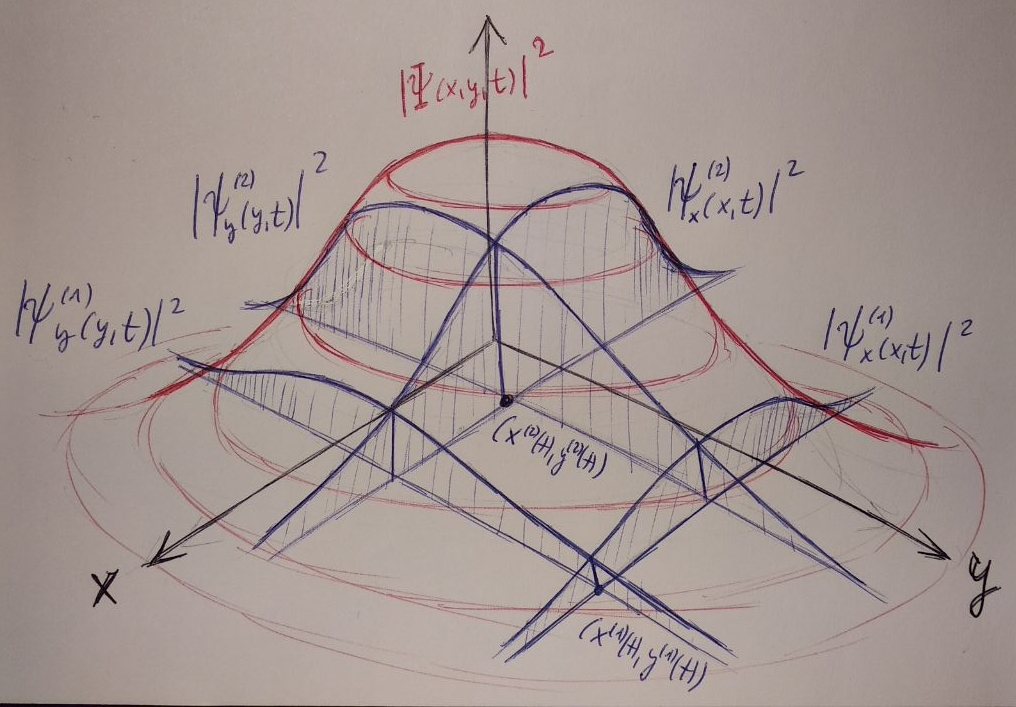
\includegraphics[width=0.65\linewidth]{slices.jpg}
  \caption{Depiction of the probability density of a 2D quantum system ($N=2$). In red the probability density of the full wave-function $\Psi(x,y,t)$ for a given time. In blue the pair of conditional wave-functions associated to two Bohmian trajectories $(x^{(1)}(t),y^{(1)}(t))$ and $(x^{(2)}(t),y^{(2)}(t))$ at a given time. Note that actually they coincide with other two trajectory's CWF-s at that time. }
  \label{fig:slices}
\end{figure}


\subsection*{Implicitly the full system is a Lagrangian fluid but explicitly only a susbsystem}
In principle, considering only $\vec{y}$ as a moving continuum would be enough to describe the complete function $f(\vec{x},\vec{y},t)$ in the Eulerian frame, employing the conditional functions $f(\vec{x},\vec{y}(\vec{\xi}_y,t),t)$. Taking enough $\vec{\xi}_y$ we would have a slice of the full function at almost all the sections of interest. However, there are several reasons that will lead us to consider that in fact, the degrees of freedom $\vec{x}$ are part of a fluid as well (just as we did in the fully Lagrangian case), just that considering them Eulerian will be convenient.

If we want to give physical meaning to the trajectories $\vec{y}(\vec{\xi}_y,t)$, each of which carries a different slice of the full function, we will have a hard interpretative dilemma. If for example, $\vec{y}$ describe the degrees of freedom of the environment and $\vec{x}$ describes the degrees of our quantum experiment: for each possible point-like configuration of the environment, moving along its trajectory $\vec{y}(\vec{\xi}_y,t)$, we will have that our Lab system is described by a continuous wavefunction $\psi(\vec{x},\vec{y}(\vec{\xi}_y,t),t)$. However, we should be able to symmetrically describe the environment using the Eulerian degrees $\vec{x}$ and our Lab in the Lagrangian degrees $\vec{y}$, since we are working with physical laws that should not depend on the region of space we are looking at (this is the main reason of all this). If we did so, then our Lab would be described by point-like configurations $\vec{y}(\vec{\xi}_y,t)$, while the environment would be a continous wavefunction $\psi(\vec{x},\vec{y}(\vec{\xi}_y,t),t)$. It seems clear that rather we describe it all using a continuity of possibilities (a wavefunction) and/or all using a set of discrete configuration trajectories. This assertion is especially sustented by the fact that each time we realize an experiment, we just find point like particles both in our Lab and in the environment, and at the same time, we observe there is interference between the continuity of possible observed configurations in both the Lab and the environment. This is precisely the justification of Bohmian Mechanics or the Tangent Universe Interpretation. 

In fact, if we try to describe the trajectory $\vec{y}(\vec{\xi}_y,t)$ using Bohmian trajectories, it will be badly undefined, because for each possible $\vec{x}$, we have a different velocity $\pdv{}{t}\vec{y}(\vec{\xi}_y,t)$ for the $\vec{\xi}_y$-th trajectory. This means that an initially univalued trajectory of the fluid element $\vec{\xi}_y$ will become multivalued, as a function of $\vec{x}$. We would be forced to describe it as $\vec{y}(\vec{\xi}_y, \vec{x},t)$. But what is the difference between this and considering directly that each position in $\vec{x}$ is as well part of a fluid element? None.

\mybox{
\subsubsection*{What if we only considered Bohmian trajectory in $\vec{y}$?}

Let us see what would happen if we insisted on only considering the Lagrangian axes as a fluid and at the same time, we tried to attribute its fluid elements a Bohmian trajectory.\\

If we define the velocity field for $\vec{y}^\xi(t)=(x_{m+1}^\xi(t), ...,x_N^\xi(t))$ to be the Bohmian velocity field for those degrees of freedom:
\begin{equation}
\dv{}{t}x_j^\xi(t)=\frac{1}{m_j}\pdv{S(\vec{x}, \vec{y})}{x_j}\Big\rvert_{\vec{y}^\xi(t)}=\frac{\hbar^2}{m_j}\Im\qty( \psi^{-1} \pdv{\psi}{x_j})\Big\rvert_{\vec{y}^\xi(t)} \quad j\in\{m+1,...,N\}
\end{equation}
We will see that for each value of $\vec{x}=(x_1,...,x_m)$, the Eulerian degrees, we have a different velocity with which to move the trajectory in $\vec{y}$. This immediately tells us that the multivalued trajectory of the fluid element $\vec{\xi}_y$, that is $\vec{y}(\vec{\xi}_y,t)$, will need to be parametrized not only by its initial position $\vec{\xi}_y$, but also by a parameter representing the point $\vec{x}$, thus $\vec{y}(\vec{\xi}_y,t; \vec{x})$. Let us re-define this parameter as $\vec{\xi}_x\equiv \vec{x}$ (for obvious reasons). Since each $\vec{\xi}_x$, or equivalently, each $\vec{x}$  only has a value of the conditional function over it, the conditional function $f(\vec{x},\vec{y}^\xi(\vec{\xi}_y,t; \vec{x}),t)$ is still a proper function in the Eulerian frame $f(\vec{x},\vec{y}^\xi(\vec{\xi}_y,t; \vec{x}),t)=f(\vec{x},t; \vec{\xi}_y)$. However, if we suddenly view what is happening from the full function's perspective, we will have started with an affine slice of the full function, but in the moment we allow each $\vec{x}$ to have a different position in $\vec{y}$, what we know about the full function is a curved slice, as can be seen in Figure \ref{fig:only_y}.

}
\begin{figure}[h!]
  \centering
    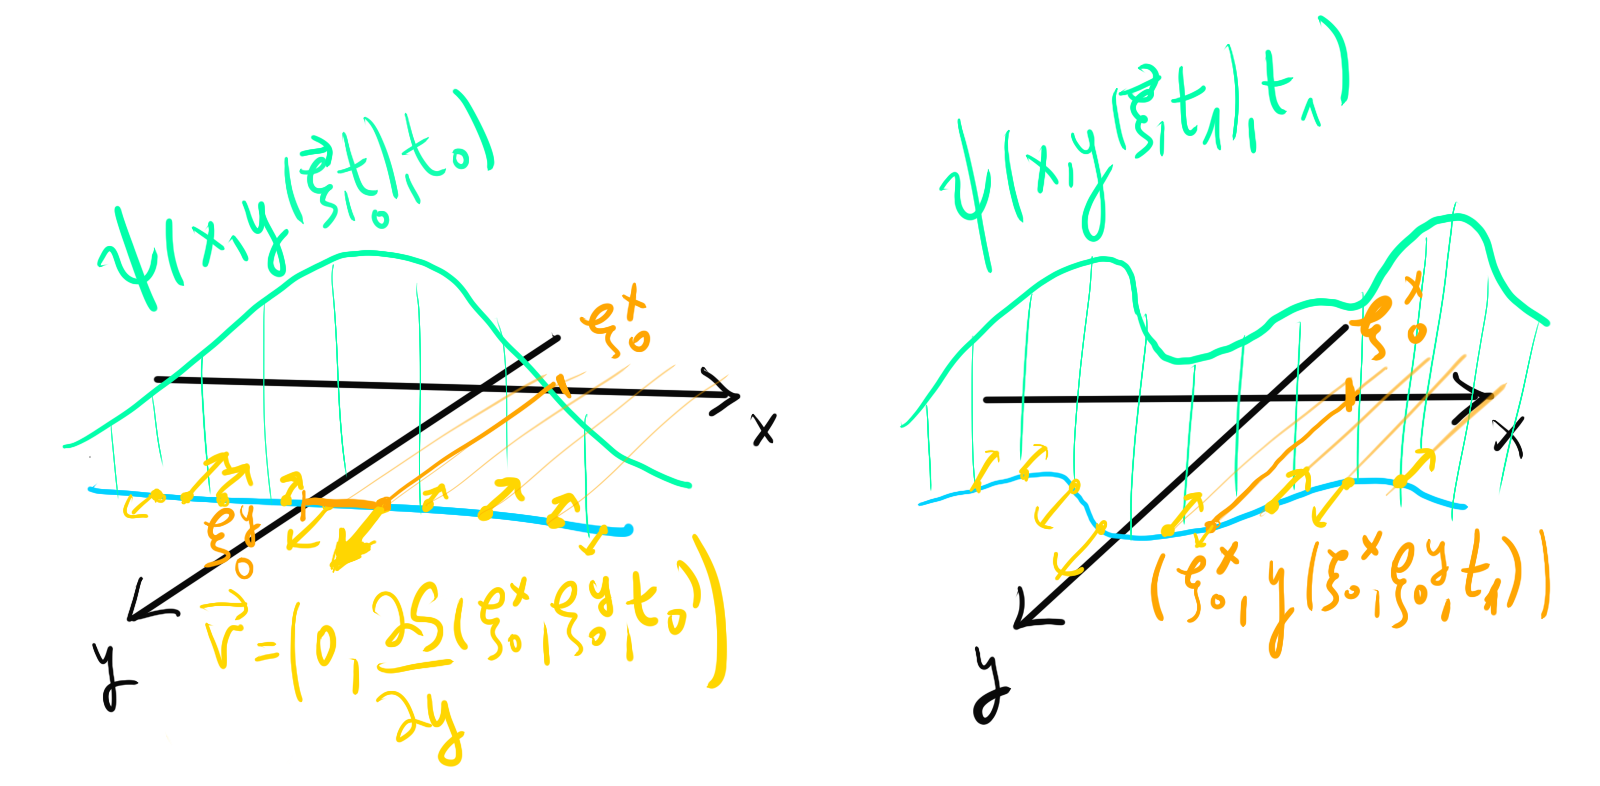
\includegraphics[width=0.65\linewidth]{unstructure_aligned.png}
  \caption{The blue line represents the $m$ dimensional support of the CWF that is conditioned to have $y=\xi^y_0$ at $t=t_0$ (in the left). In green we see the magnitude of the complex CWF plotted over the support of the CWF (the slice of the full WF). In yellow we see the velocity vectors that will move each element of the CWF, each parametrized $\xi^x_j$. We see in the right the time $t_1>t_0$. Note haow the elements $\xi^x_j$ always preserve their $x=\xi^x_j$ value, that is, they strictly move in $y$. }
  \label{fig:only_y}
\end{figure}
\mybox{
In principle there is no problem, since as said, the conditional function has still a single value per $\vec{x}$, so it would be a valid Eulerian function. Does this mean we really achieve the evolution of Bohmian trajectories of the sub-system $\vec{y}$ only evolving this subsystem in a Lagrangian way? Not really. We are restricting the movement of the fluid elements to be still in $\vec{x}$, but the Bohmian velocity in $\vec{y}$ also depends on $\vec{x}$, so if in reality there should be displacement in $\vec{x}$ and we do not account for it, whatever the trajectories we get, they are not Bohmian.\footnote{
Even if it will not be the approach we will use because it has a big problem to reconcile with Bohmian trajectories, as the equations for the conditional functions will be equivalent considering only $\vec{y}$ as a fluid or not, let us remark the main computational benefit of considering as a fluid only the subsystem $\vec{y}$. If we evolved several conditional functions for different initial positions in $y^\xi(t_0)=\xi^y_k$, the discretized $x$ points would always be aligned between the conditional functions, with the advantage that computing derivatives $\pdv{}{y}$ or interpolating in $y$ would be way simpler, even if the $y$ grid for each $x$ would get not equispaced with time. See Figure \ref{fig:only_y_grid}} From the Fully Lagrangian perspective, what we are doing is:
\begin{equation}\label{a}
\begin{cases}
\vec{x}(\vec{\xi}_y, \vec{\xi}_x,t)=\vec{\xi}_x \quad \forall t\geq t_0\\
\vec{y}(\vec{\xi}_y, \vec{\xi}_x,t)=\vec{\xi}_y+\int_{t_0}^t \vec{v}_y(\vec{x}=\vec{\xi}_x, \vec{y}=\vec{y}(\vec{\xi}_y, \vec{\xi}_x,t),t)dt\\ \\
v_j(\vec{x}, \vec{y},t)=\frac{1}{m_j}\pdv{S(\vec{x}, \vec{y},t)}{x_j}\quad j\in\{m+1,...,N \}
\end{cases}
\end{equation}
}
\begin{figure}[h!]
  \centering
    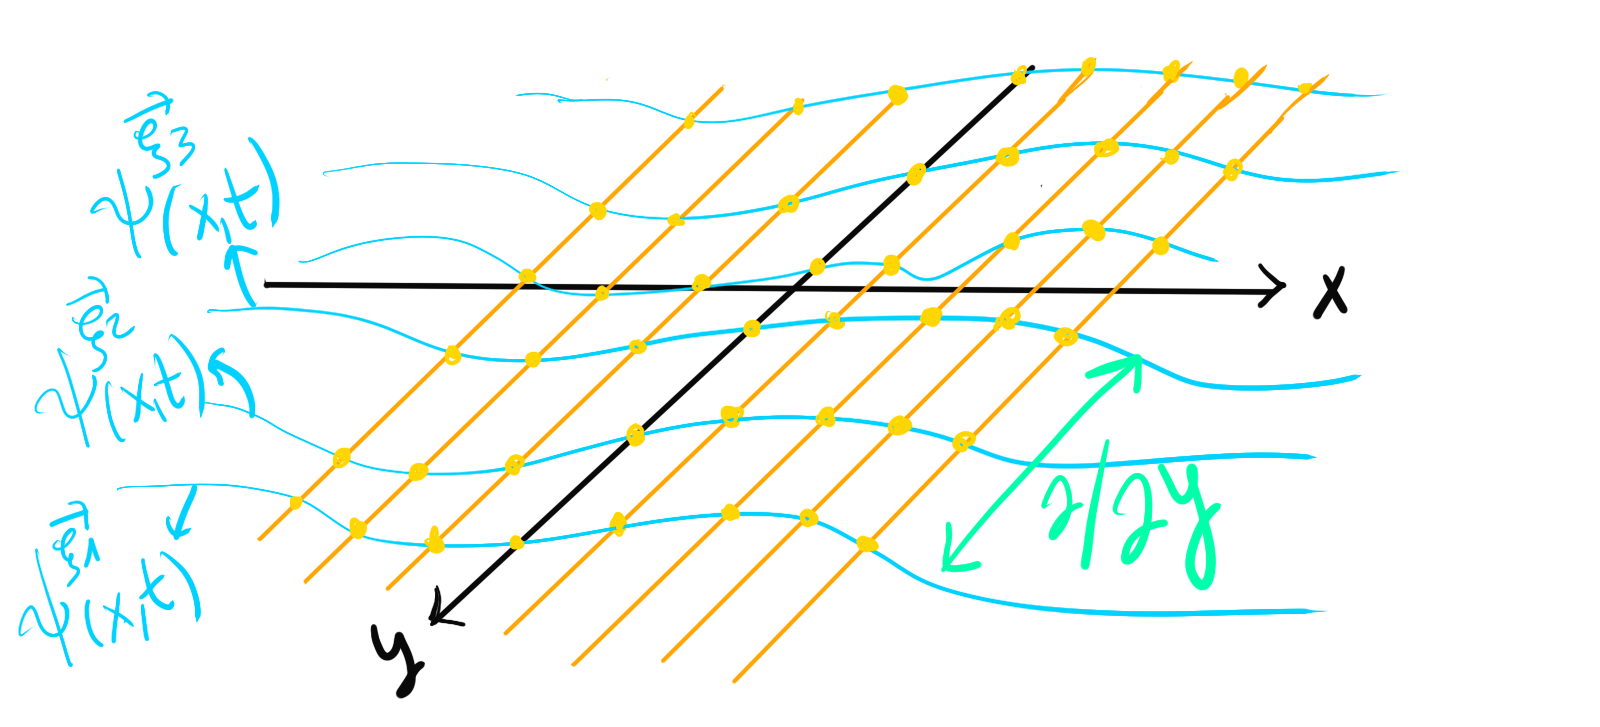
\includegraphics[width=0.65\linewidth]{aligned.png}
  \caption{Blue lines represent the suppoort of CWF-s with different initial time $\xi^y_j$ after they evolve in time following  \eqref{a}. Note how the discretized points of all the CWF-s, the yellow dots, are aligned even at $t>t_0$, meaning operations like $\pdv{}{y}$ on each yellow element can be trivially done numerically. }
  \label{fig:only_y_grid}
\end{figure}
\mybox{
\subsection*{Falling back to the Fully Lagrangian Picture}
Thus, to really get Bohmian trajectories, we should allow the points in $\vec{x}$ to move as well, this would allow the fluid elements in $\vec{y}$ to have the correct Bohmian velocity. But what if we allowed {\bf all of them} to move in the direction given by the Bohmian velocity field? We would have that:
\begin{equation}
\begin{cases}\label{b}
\vec{x}^\xi(t)=\vec{\xi}_x +\int_{t_0}^t \vec{v}_x(\vec{x}(t), \vec{y}(t),t)dt\quad \forall t\geq t_0\\
\vec{y}^\xi(t)=\vec{\xi}_y+\int_{t_0}^t \vec{v}_y(\vec{x}(t), \vec{y}(t),t)dt\\ \\
v_j(\vec{x}, \vec{y},t)=\frac{1}{m_j}\pdv{S(\vec{x}, \vec{y},t)}{x_j}\quad j\in\{1,...,N \}
\end{cases}
\end{equation}

As it can be seen in Figure \ref{fig:fallback}, each element of the initially affine Eulerian support of the conditional function (blue in the Figures), would move in different directions in the $N$ axes of configuration-space. We would end up having a varying number of values of the same function $f$ for a same $x$, which is incompatible with the Eulerian view. The function in $\vec{x}$ would become multivalued. The support would still be an $m$ dimensional manifold, meaning the parametrization given by $\vec{\xi}_x$ would still be valid, and we would still have one point in the wavefunction per each $\vec{\xi}_x$ in the initial manifold. However, a value per fluid element is exactly what we had in the Fully Lagrangian Picture $f(\vec{x}(\vec{\xi},t), \vec{y}(\vec{\xi},t),t)=f(\vec{\xi},t)$.
}
\begin{figure}[h!]
  \centering
    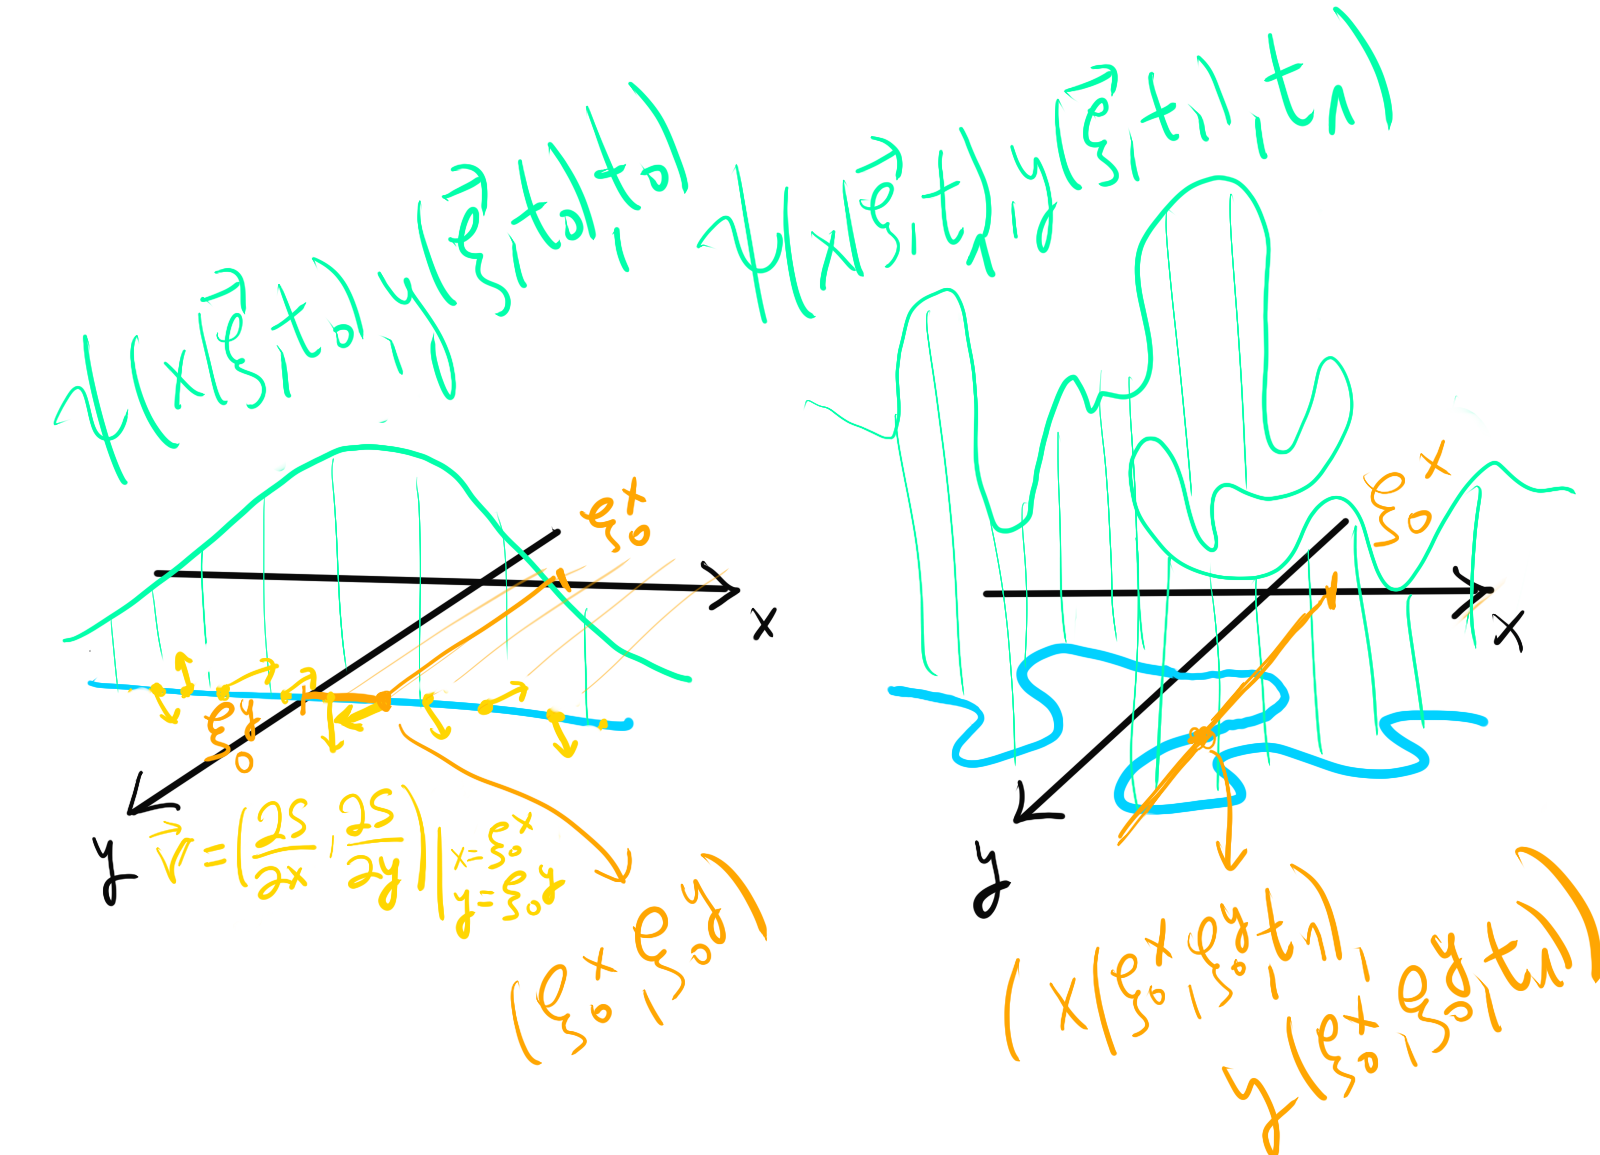
\includegraphics[width=0.65\linewidth]{unstructuring.png}
  \caption{Left $t=t_0$, right $t=t_1$. In blue, the $m$ dimensional support of the CWF. In green the field value at each point (say the phase or magnitude of the WF). In yellow the elements of the CWF we consider, together with the velocity vectors we will use to move them according to \eqref{b}. Note how each fluid element moves independently, unstructuring the grid they compose not only in $y$ as happened in (a), but also in $x$, just like with the fully Lagrangian study-case. }
  \label{fig:fallback}
\end{figure}

\mybox{
\subsection*{Solution: Evolve a single $\R^N$ Bohmian trajectory per conditional function}
We have found that having really Bohmian trajectories move each point of the conditional function resulted in the fully Lagrangian frame. However, notice that this was only because we allowed each point of the support to move independently. What if we forced all the points of the support of the conditional function to move along a single Bohmian trajectory? We would then achieve our original idea. If we only associate a single Bohmian trajectory to the evolution of a conditional function, we will have a partially Eulerian description consistent with Bohmian trajectories. See Figure \ref{fig:singleTraj}. 

}
\begin{figure}[h!]
  \centering
    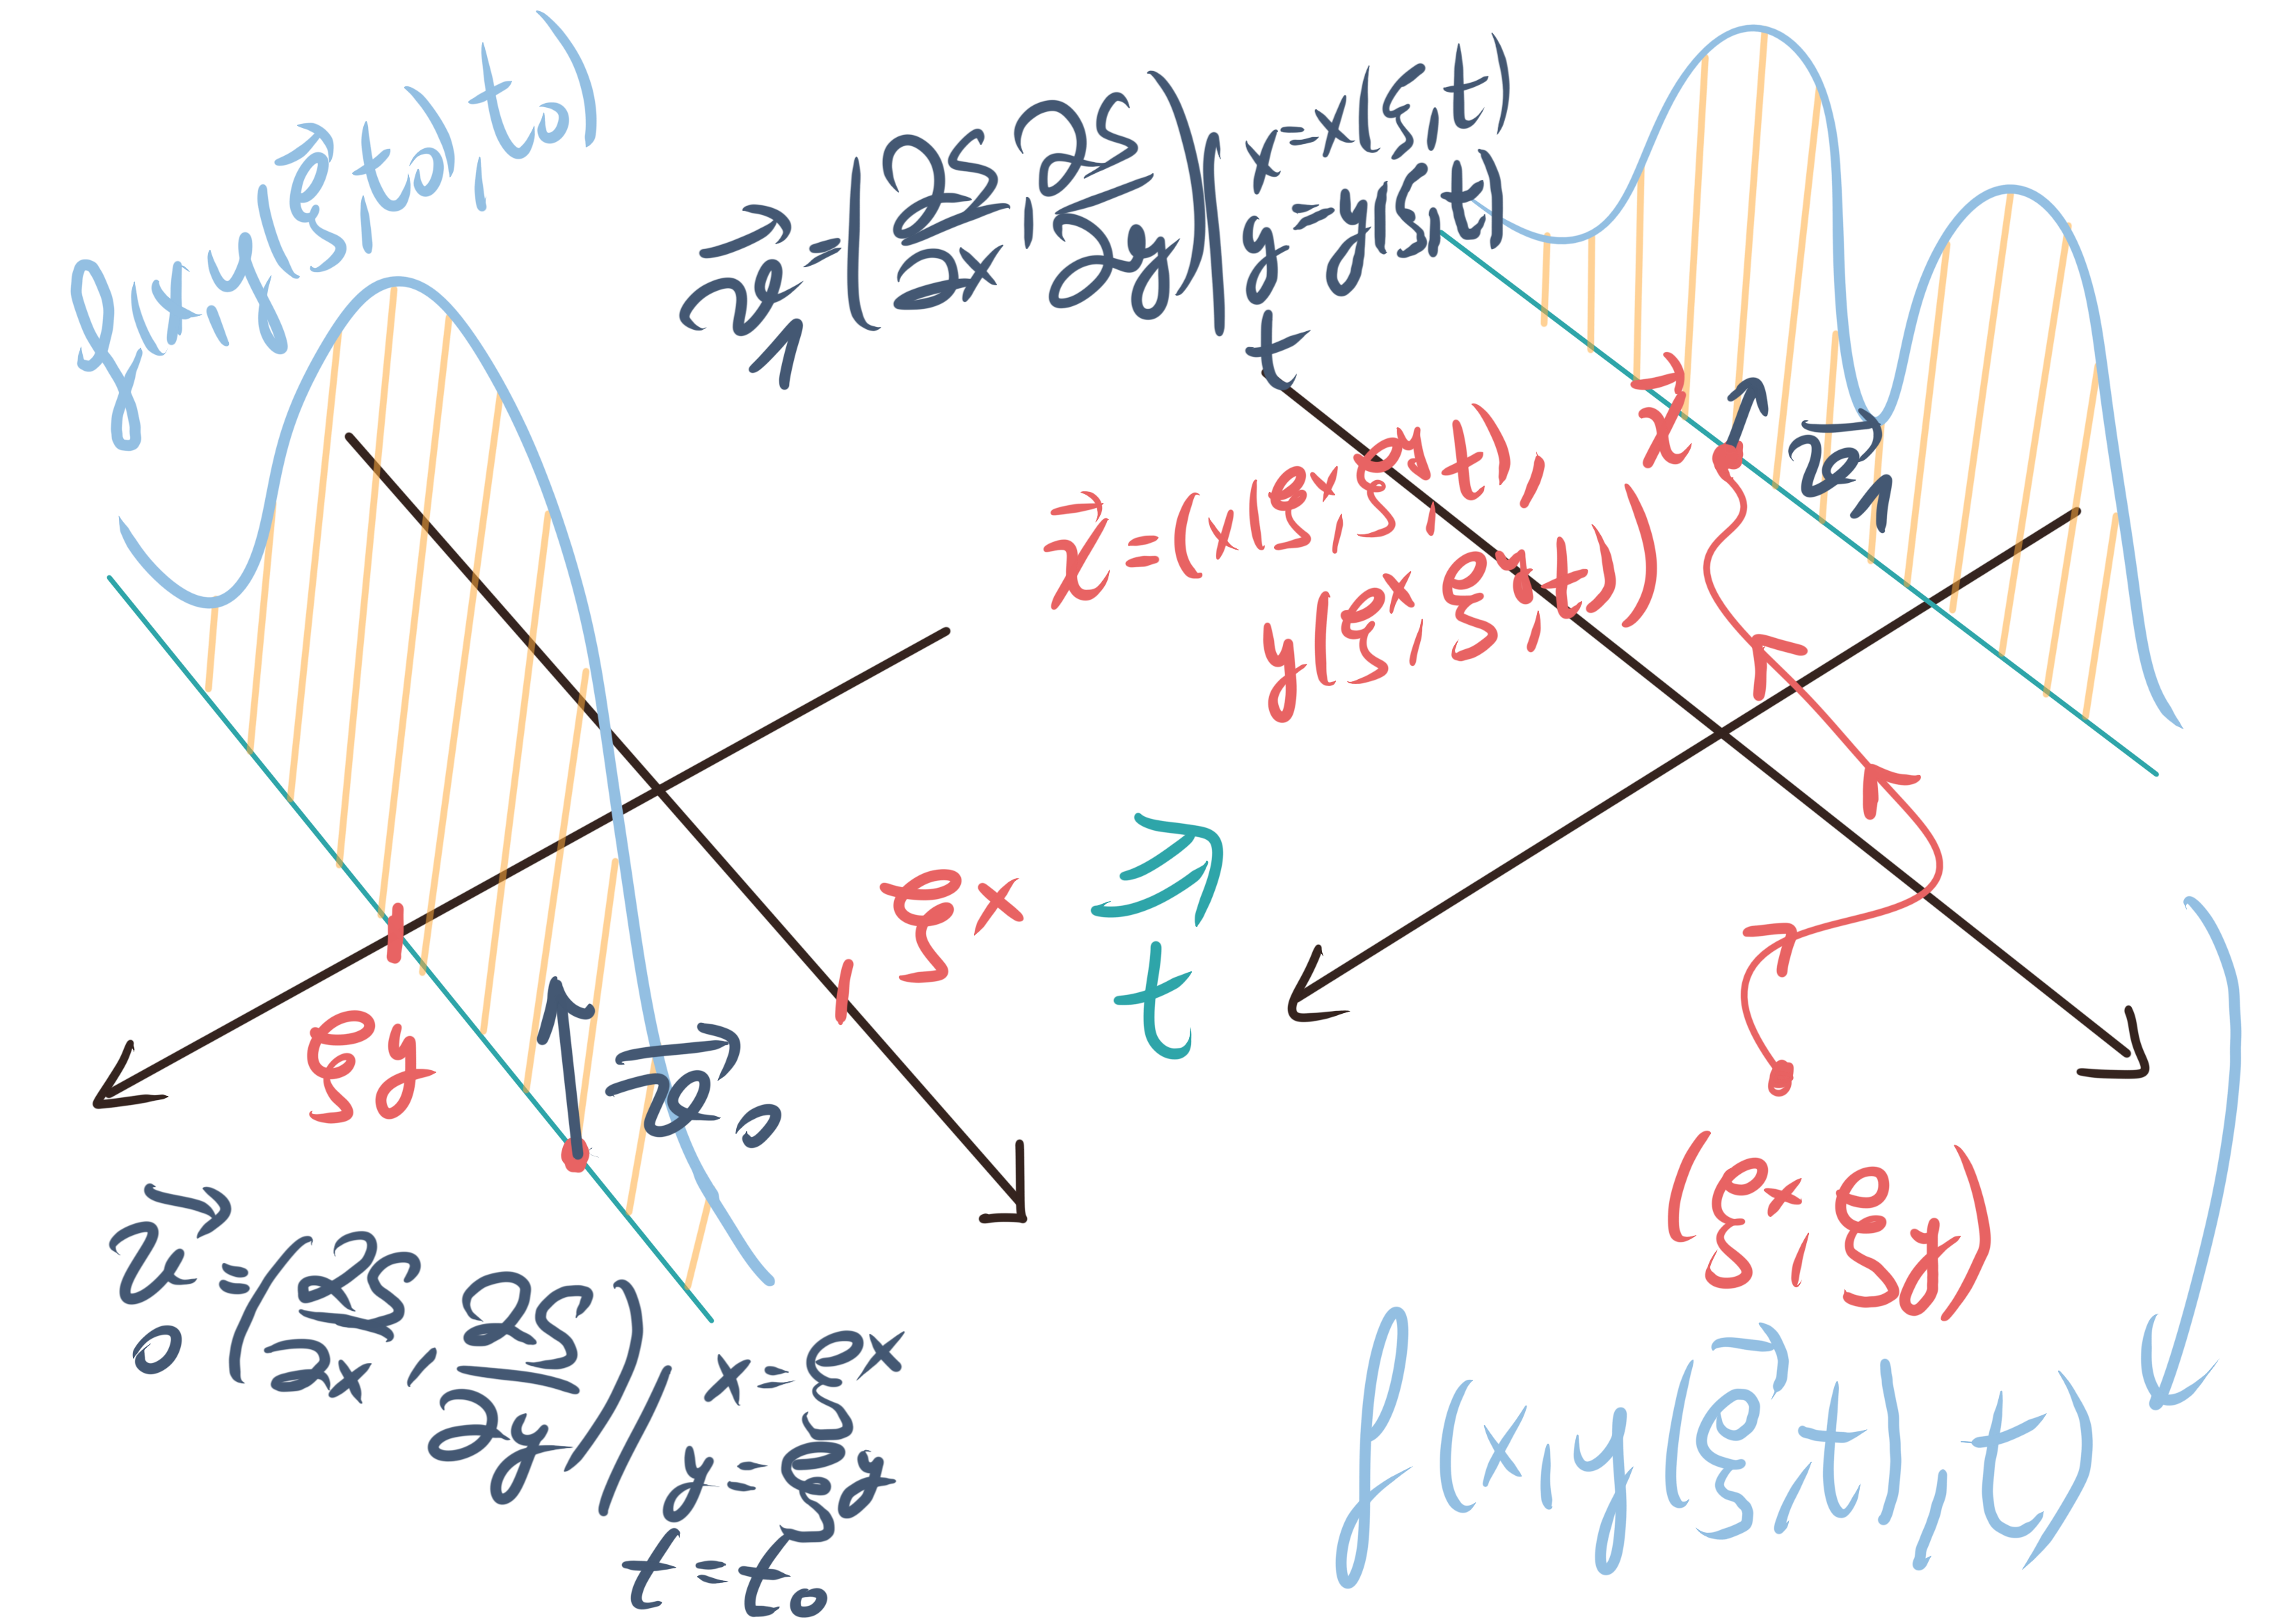
\includegraphics[width=0.65\linewidth]{moving_bohmian.png}
  \caption{Right $t=t_0$, left $t=t_1$. In blue, the support of the CWF, which can be seen to have its affinity preserved at all times. This is because the whole CWF is displaced following the same Bohmian trajectory as explained in (c): the one for $(\xi^x_0, \xi^y_0)$. In green the value of a property of the WF over the support of the CWF. We see that the $x$ velocity of the trajectory is fully given by the variation of the CWF. For the velocity in $y$ however, we still have the problem that we are only dealing with a single slice and thus cannot have local information of first or higher order. }
  \label{fig:singleTraj}
\end{figure}

Therefore, for both allowing a homogeneous interpretation of physics and allowing the coupled description of a conditional function with Bohmian trajectories in the full configuration-space (which seem ontologically the most interesting trajectories we can get), we will consider the whole space $\vec{\x}\in\Omega_t\subseteq\R^N$ to be a fluid composed of $N$-dimensional point-like fluid elements, just that we will still consider conditional functions, for their potential benefits.

For this, we will use $\vec{\xi}_x=(\xi_1,...,\xi_m)$ to denote the Lagrangian labels of the degrees of freedom treated in the Eulerian frame $\vec{x}$, while $\vec{\xi}_y=(\xi_{m+1},...,\xi_N)$ will denote the labels of the Lagrangian degrees of freedom. In general, to uniquely identify a fluid element and its associated conditional function, we will not have enough with $\vec{\xi}_y$, but will require the full label $\vec{\xi}=(\vec{\xi}_x,\vec{\xi}_y)\in \Omega_0\subseteq\R^N$. This means that now the continuous velocity field driving the fluid elements can be dependent on $\vec{x}$, meaning there will be a diffeomorphism describing the trajectories for the full system $\vec{\x}(\vec{\xi},t)=(\vec{x}(\vec{\xi},t), \vec{y}(\vec{\xi},t))$. 

Very importantly, whenever we consider a conditional function $f(\vec{x},\vec{y}(\vec{\xi},t),t)$, we will also be able to conceive another conditional function "coupled" to the first through the trajectory of a same fluid element $\vec{\xi}$, namely $f(\vec{x}(\vec{\xi},t),\vec{y},t)$. In fact, we could consider several conditional functions, until $N$, each with a different dimensionality. For example, we could consider $f(x_1(\vec{\xi},t),x_2(\vec{\xi},t),x_3,...,x_N,t)$, $f(x_1, x_2, x_3(\vec{\xi},t), x_4,...,x_N)$ and $f(x_1, x_2, x_3, x_4(\vec{\xi},t),...,x_N(\vec{\xi},t))$. In general, we will call these conditional functions coupled by parts of the same trajectory, {\bf complementary conditional functions}. Interesting particular cases will be:
\begin{itemize}
\item Having $N$ complementary conditional functions, one per each degree $x_k$, describing the function conditioned to the rest of the system being in a given trajectory. Meaning that each degree of freedom will be described by a 1D Eulerian function and a point-like position $x_k(\vec{\xi},t)$.
\item Having $N/3$ complementary conditional functions, one per triad of degrees of freedom. This way, we could have a 3D function describing each physical space particle, together with its 3D position $(x_{k}(\vec{\xi},t), x_{k+1}(\vec{\xi},t),x_{k+2}(\vec{\xi},))$, where $\vec{\xi}$ would reflect its initial position and the initial position of the rest of the particles in the system. For each possible initial position of the system, we would have a different set of 3D functions and trajectories for the system, which unfortunately from the ontological perspective, will influence each other contingently (they will push each other as we already saw).
\item Having 2 complementary conditional functions: one for our lab system and one for the rest of the particles in the Universe (the environment). We would then have a wavefunction for the lab system and a wavefunction for the environment, both coupled through the common global trajectory of the system.
\end{itemize} 
Hereafter, we will assume when describing a conditional function that along with it, we also evolve the rest of complementary conditional functions associated to its trajectory.

Note that if we consider the set of complementary conditional functions for a given discretized grid of fluid elements $\{\vec{\xi}^j\}_{j=1}^M$, we will have that for all the fluid elements that at a certain time turn to be aligned along any $x_k$ axis, their conditional functions in that axis will be exactly the same. See Figure \ref{fig:over} for a visual understanding. This means that we will have an over-representation of the "slices" of the full function. In the numerical/computational approaches, this will not be something to really worry about, since the positions being real numbers makes it is hardly impossible to have more than one trajectory passing from the same $x_k$ point at the same time. However, in theory an infinite amount of trajectories cross the same point in $x_k$ at the same time, which is why we rise up this over-representation warning.



\begin{figure}[h!]
  \centering
    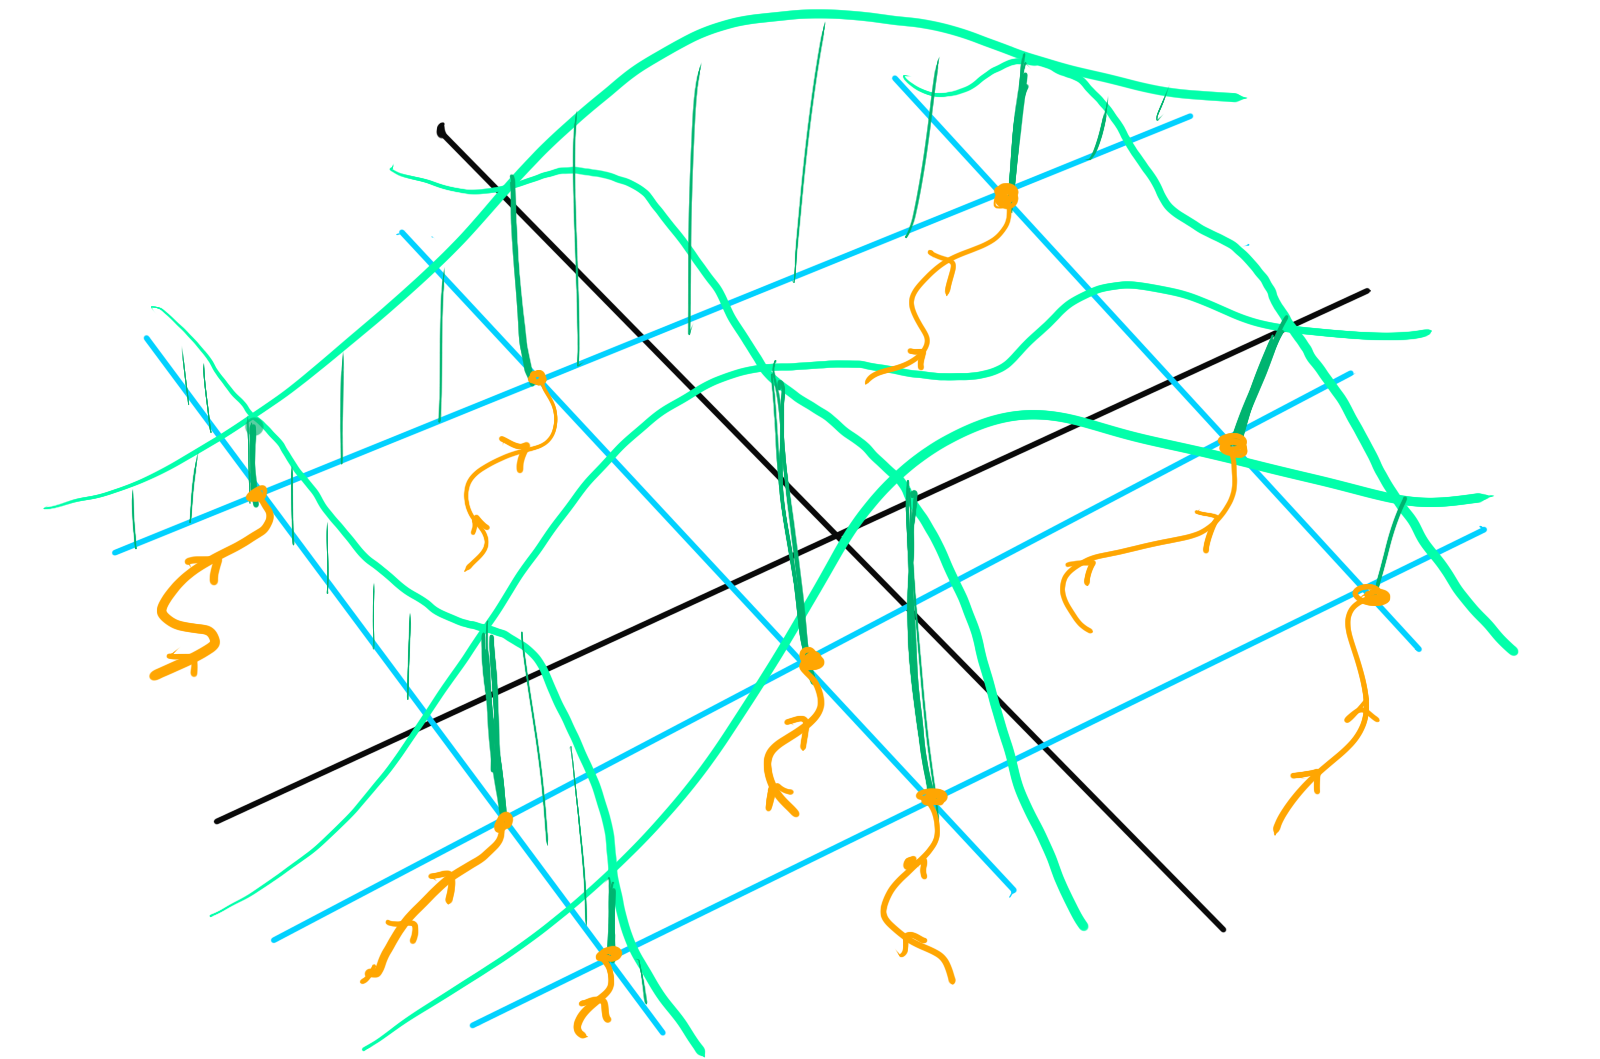
\includegraphics[width=0.65\linewidth]{many_bohmian.png}
  \caption{In blue we can see the affine supports of several pairs of CWF-s (slices of the WF) built by following \eqref{d}. In each intersection we have enough information as for evolving a Bohmian trajectory. }
  \label{fig:over}
\end{figure}

\subsection*{Why some Bohmian believe the Complementary Conditional Functions and their Trajectory are the {\em arkhe}?}

Following the expression for the velocity field guiding the fluid elements \eqref{v}, for the movement in any Eulerian axis $x_k$, the velocity field only depends on the derivative of the action in that same direction $\pdv{}{x_k}$. This means that we have enough with the conditional wavefunction $\psi(\vec{x},\vec{y}(\vec{\xi},t),t)$ to know the trajectory of the coupled fluid element $\vec{\xi}$ in the $\vec{x}$ degrees of freedom. This somewhat suggests that if the Bohmian trajectory is the ultimate ontological reality and if the complementary conditional functions (the wavefunction or the aciton and density) of a certain trajectory are the only necessary functions to predict its motion, then there must be some serious weight in those complementary conditional functions. 

\begin{figure}[h!]
  \centering
    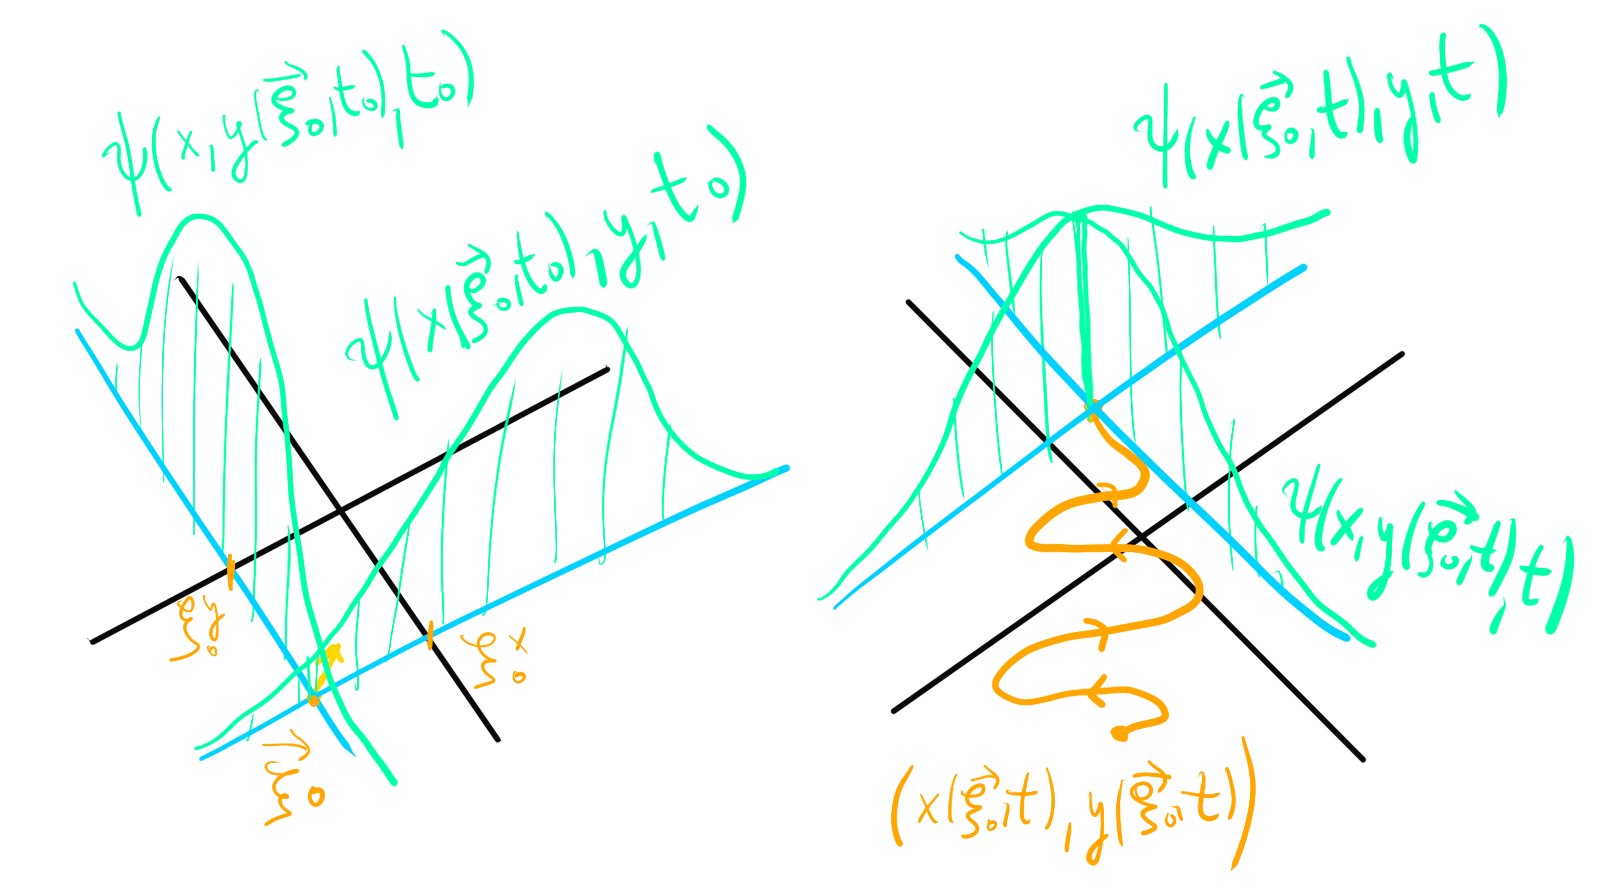
\includegraphics[width=0.65\linewidth]{bohmian_pair.png}
  \caption{Following the same caption of Figure \ref{fig:singleTraj}, we see that having a complementary CWF that has as Lagrangian degrees of freedom the Eulerian ones of the first, allows the evolution of the common trajectory with no further requirements. Note how the WF value at the trajectory position for both CWF-s should coincide. The difference of these could be a metric to be used in numerical simulations.  }
  \label{fig:pair_bohm}
\end{figure}

It is however somewhat fallacious to say this, since as we will see, the equations that predict the motion of those complementary conditional functions that are the only thing affecting the trajectory, actually depend on the rest of possible complementary conditional functions. This will be because their time evolution will require the knowledge of the derivatives $\pdv{}{x_k}$ of the Lagrangian axes, but since we are considering with each conditional function a single slice, we will not have enough information. We will have it at the exact point of the trajectory $\vec{x}^\xi(t)$ coupling them, but not in all the rest of positions in $\vec{x}$.

Nonetheless, we will see in a moment a formidable way to hide this dependency even further away from the trajectories, by first defining the $G,J$ correlation potentials, and then defining dynamical equations for them.

\newpage
\subsection*{(III.a.1) The Schrödinger Equation: Kinetic and Advective Correlation Terms}
\addcontentsline{toc}{subsubsection}{{\bf (III.a.1)} The Schrödinger Equation: Kinetic and Advective Correlation Terms}
If we evaluate $\vec{y}=\vec{y}(t,\vec{\xi})$ in the Schrödinger Equation \eqref{SE}, leaving $\vec{x}$ in the Eulerian frame:
\begin{equation}
i\hbar \pdv{}{t}\psi(\vec{x}, \vec{y}^\xi(t),t)=-\sum_{j=1}^m \frac{\hbar^2}{2m_j}\pdv[2]{}{x_j} \psi(\vec{x}, \vec{y}^\xi(t),t) + U(\vec{x}, \vec{y}^\xi(t),t)\psi(\vec{x}, \vec{y}^\xi(t),t) -\sum_{j=m+1}^N \frac{\hbar^2}{2m_j}\pdv[2]{}{x_j} \psi(\vec{x}, \vec{y},t)\Big\rvert_{\vec{y}^\xi(t)}
\end{equation}
Using that by the chain rule:
\begin{equation}
\dv{}{t}\psi(\vec{x}, \vec{y}^\xi(t),t)=\pdv{}{t}\psi(\vec{x}, \vec{y}^\xi(t),t)+\sum_{j=m+1}^N \pdv{}{x_j}\psi(\vec{x}, \vec{y},t)\Big\rvert_{\vec{y}^\xi(t)}\cdot \dv{}{t}x^\xi_j(t)
\end{equation}
We get:
\begin{equation}\label{KinAdvEL}
i\hbar \dv{}{t}\psi(\vec{x}, \vec{y}^\xi(t),t)=\qty[-\sum_{j=1}^m \frac{\hbar^2}{2m_j}\pdv[2]{}{x_j} + U(\vec{x}, \vec{y}^\xi(t),t)]\psi(\vec{x}, \vec{y}^\xi(t),t)+K(\vec{x}, \vec{y}^\xi(t),t)+A(\vec{x}, \vec{y}^\xi(t),t)
\end{equation}

Where we define the so called Kinetic and Advective correlation potentials:
\begin{equation}\label{KinEL}
K(\vec{x}, \vec{y}^\xi(t),t):=-\sum_{j=m+1}^N \frac{\hbar^2}{2m_j}\pdv[2]{}{x_j} \psi(\vec{x}, \vec{y},t)\Big\rvert_{\vec{y}^\xi(t)}
\end{equation}
\begin{equation}\label{AdvEL}
A(\vec{x}, \vec{y}^\xi(t),t):=i\hbar\sum_{j=m+1}^N \pdv{}{x_j}\psi(\vec{x}, \vec{y},t)\Big\rvert_{\vec{y}^\xi(t)}\cdot \dv{}{t}x^\xi_j(t)
\end{equation}
We can see that equation \eqref{KinAdvEL} ruling the motion of the conditional wavefunction $\psi(\vec{x}, \vec{y}^\xi(t),t)$ is almost a Schrödinger Equation for a system of $m$ (instead of $N$) dimensions. The difference is that we now have two additional affine terms that actually depend on derivatives of the full wavefunction in the axes that we are considering in the Lagrangian frame. As we already anticipated that would happen, if we want to evolve a single conditional wavefunction (or the complementary conditional wavefunction set it is part of), we do not have enough with themselves. We would require the knowledge of complementary conditional wavefunctions of other trajectories. It is just the same problem that we faced with the fully Lagrangian picture. As such, to solve this problem we will be able to use the same strategies: 
\begin{itemize}
\item Evolve several trajectories and their conditional wavefunctions and use them as a discretized version of the full wavefunction to get the derivatives for each trajectory. We would still have the problem that the grid would become non-equispaced, even if the unstructuring in this case would be better, since each single conditional function is already a whole set of points of what the Fully Lagrangian picture allowed.

To do this we could change the derivatives in $x_k$ to derivatives in the label space $\xi_k$, which we could choose to be equispaced, fit a sum of analytic functions and compute the derivatives symbolically or use a $K$ nearest neighbourgh apporach to predict the full wavefunction and make numerical derivatives etc.

\item Evolve the derivatives of the wavefunction along the trajectories with a chain of infinite differential equations, or similarly evolve the Kinetic and Advective correlation potentials.
\end{itemize}

\begin{figure}[h!]
  \centering
    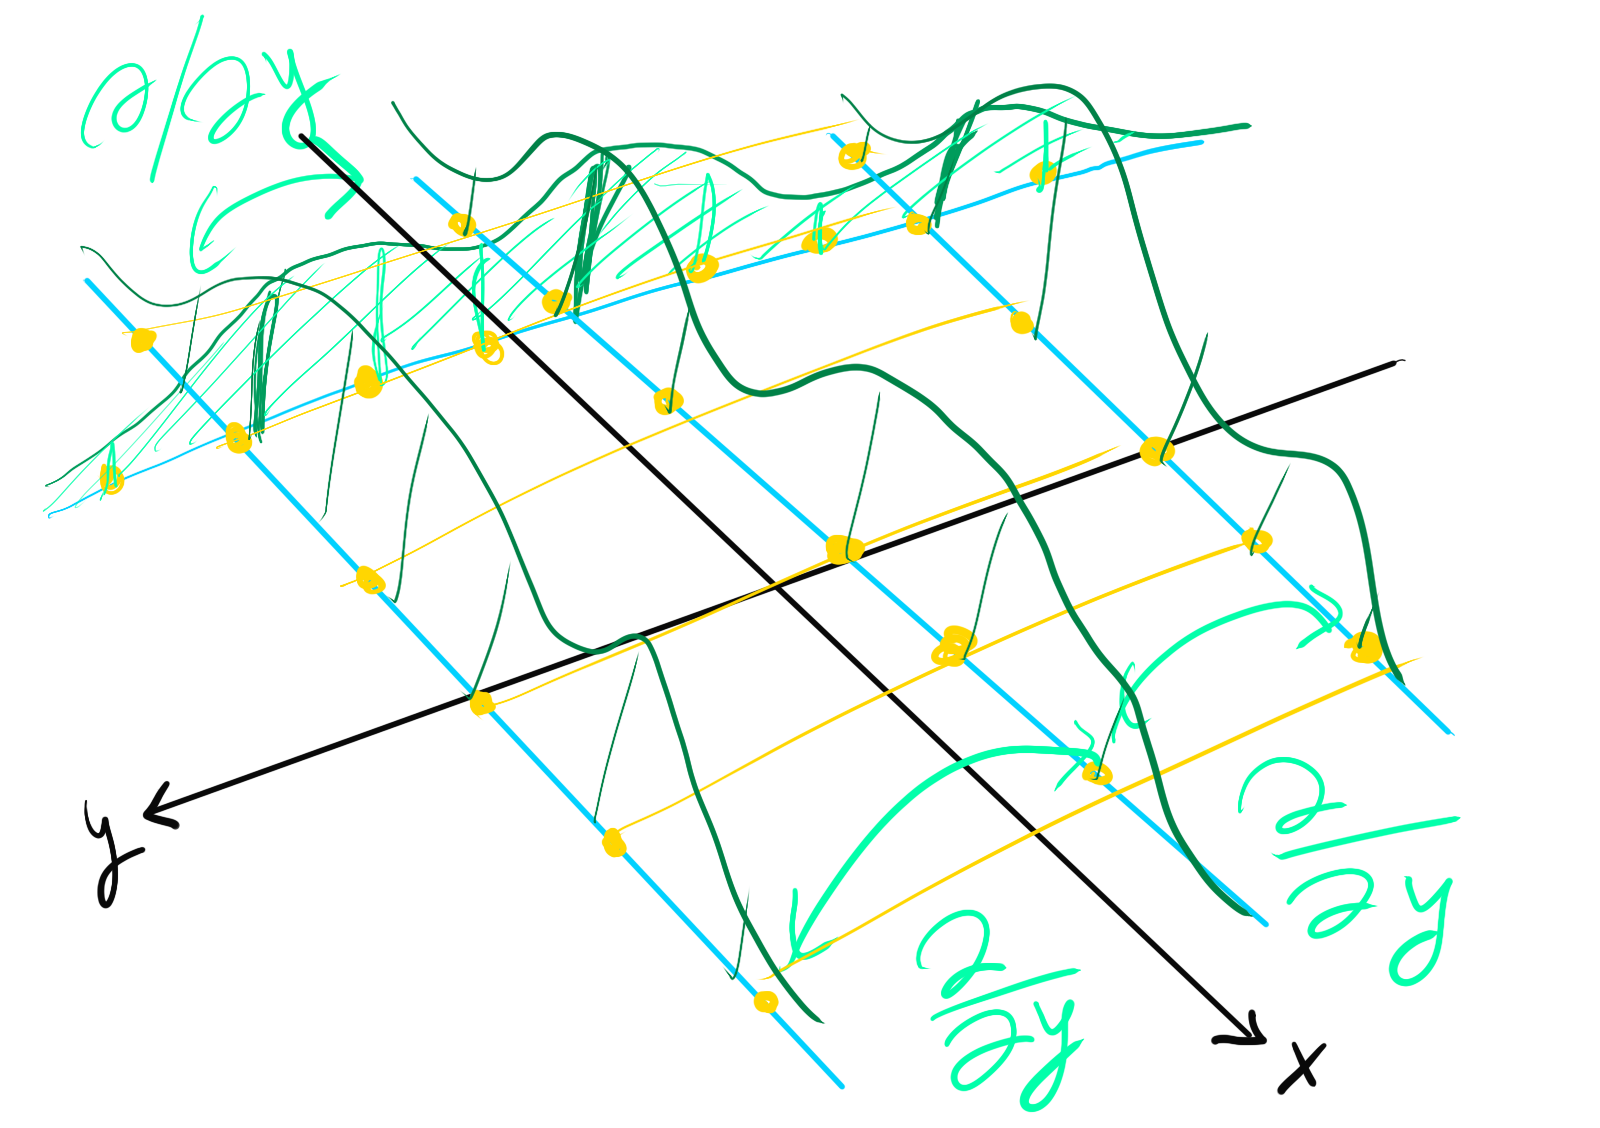
\includegraphics[width=0.65\linewidth]{aligned_original.png}
  \caption{In blue we can see several CWF-s (their supports). Yellow dots show the discrete elements of the CWF-s we will consider. This image shows two things: 1. parallel CWF-s (CWF-s with the same Lagrangian degrees but different initial positions) can be used to approximate derivatives in the Lagrangian directions $\pdv{}{y}$. 2. Crossed CWF-s with complementary Lagrangian degrees can be used also to approximate derivatives in the Lagrangian directions with a higher degree of precision than using parallel CWF-s.  }
  \label{fig:aligned2}
\end{figure}


\subsection*{(III.a.2) The Schrödinger Equation: G and J Correlations}
\addcontentsline{toc}{subsubsection}{{\bf (III.a.2)} The Schrödinger Equation: G and J Correlations}
In this section we will develop a Schrödinger-like equation for the conditional wavefunctions (CWF) that this time will be a linear one, unlike the Kinetic and Advective equation \eqref{KinAdvEL}. An interesting part will be that the Lagrangian degrees of freedom will be required in density and action shape, while the Eulerian part will be required in wavefunction shape. 

Following the development in Chp.1 V 6 of \cite{JordiXO}, we can try to find a Schrödinger like equation for the CWF-s employing the following "trick". An arbitrary non-zero single valued complex function $f(x, t):\R^m \rightarrow \C$ can be imposed to be the solution of an mD Schrödinger equation:\vspace{-0.3cm}
$$
i \hbar \pdv{f(x,t)}{t} = -\sum_{k=1}^m\frac{\hbar^2}{2 m_k}\pdv[2]{f(x,t)}{x_k} + W(x,t) f(x,t)
$$
if the potential term $W(x, t)$ is defined as:\vspace{-0.3cm}
$$
W(x, t) := \qty(i \hbar \pdv{f(x,t)}{t} +\sum_{k=1}^m\frac{\hbar^2}{2 m_k}\pdv[2]{f(x,t)}{x_k} ) \frac{1}{f(x,t)}\vspace{-0.3cm}
$$
The proof is immediate. An observation that we must note is that for an arbitrary $f(x,t)$, the potential $W(x,t)$ can be complex. This is not the case in the usual Schrödinger Equation.

If we now take the CWF where we had $m$ Eulerian degrees of freedom $x$ and $N-m$ Lagrangian degrees of freedom $y$ and write it in polar form: $\psi(x, y^\xi(t),t)=:\psi^\xi (x,t)=\p^\xi(x,t) e^{i\z^\xi(x,t) / \hbar}$, we can introduce it in this general complex potential $W^\xi(x,t)$:
$$
W^\xi(x, t) = \qty(i \hbar \pdv{\psi^\xi (x,t)}{t} +\sum_{k=1}^m\frac{\hbar^2}{2 m_k}\pdv[2]{\psi^\xi (x,t)}{x_k} ) \frac{1}{\psi^\xi (x,t)} = \qty(i \hbar \pdv{\qty(\p^\xi e^{i\z^\xi/\hbar})}{t} +\sum_{k=1}^m\frac{\hbar^2}{2 m_k}\pdv[2]{\qty(\p^\xi e^{i\z^\xi/\hbar})}{x_k} ) \frac{1}{\p^\xi e^{i\z^\xi/\hbar}}
$$
using the Leibniz derivation rule several times and an inverse chain rule, rearranging we arrive at:
$$
W^\xi(x, t)=-\sum_{k=1}^m\frac{1}{2m_k} \qty( \qty(\pdv{\z^\xi}{x_k})^2 -\frac{\hbar^2}{\p^\xi}\pdv[2]{\p^\xi}{x_k})\ -\pdv{\z^\xi}{t}+ \ i \ \frac{\hbar}{\p^{\xi\ 2}} \qty(\pdv{\p^{\xi\ 2}}{t}+\sum_{k=1}^m\pdv{}{x_k}\qty(\frac{\p^{\xi\ 2}}{m_k}\pdv{\z^\xi}{x_k}))
$$
%Separating the real and imaginary parts:
%$$
%\begin{cases}
%\mathbb{R}e\{W(x,t)\}=-\pdv{\z^\xi(x,t)}{t}-\frac{1}{2m_a} \qty( \qty(\pdv{\z^\xi(x,t)}{x_a})^2 -\frac{\hbar^2}{\p^\xi(x,t)}\pdv[2]{\p^\xi(x,t)}{x_a})\vspace{-0.3cm} \\ \\
%\mathbb{I}m\{W(x_a, t)\} = \frac{\hbar}{\p^\xi(x,t)^2} \qty(\pdv{\p_a^2}{t}+\pdv{}{x_a}\qty(\frac{\p_a^2}{m_a}\pdv{\z_a}{x_a}))\vspace{-0.1cm}
%\end{cases}
%$$
%Where we can recognize the \ref{QHJE} for a single particle in 1D. As such, the real part of W is simply the scalar real potential, then the Hamiltonian, followed by the kinetic energy and the quantum potential of a 1D particle.
%Which is clearly a modified particle conservation equation \ref{CE}. Note how if  $Im\{W(x_a, t)\} =0$ then we get the common continuity equation, which would mean that probability is conserved, and the solution $\Phi(x,t)$ would preserve its norm at all times (the conditional $r_a^2$ would integrate a same norm at all times in its spatial dimension $x_a$). Nonetheless, if $Im\{W(x_a, t)\} \neq 0$, then particles/probability are NOT conserved, and their source or sink will be quantified by $\frac{2 \_a^2}{\hbar} Im\{W(x_a, t)\}$. Therefore, the norm of $\psi^\xi (x,t)$ will not need to be preserved in the time evolution. \vspace{-0.3cm}\\

If $W^\xi$ has that shape, $\psi^\xi (x,t)$ will be the solution of the differential equation:\vspace{-0.2cm}
$$
i \hbar \pdv{\psi^\xi (x,t)}{t} = -\sum_{k=1}^m \frac{\hbar^2}{2 m_k}\pdv[2]{\psi^\xi (x,t)}{x_k} + W^\xi(x,t) \psi^\xi (x,t)\vspace{-0.2cm}
$$
which if $\mathbb{I}m\{W^\xi\} =0$ would look like an actual mD Schrödinger Equation. However, $W^k$ depends on parts of the CWF itself, so the differential equation is  {\bf non-linear} even in that case.

We can further develop the expression of $W^\xi$ using the conditional definition of $\psi^\xi$. Note that $\psi^\xi ( x, t) := \Psi(x, y^\xi(t),t)$ means that $\z^\xi(x,t)=S(x, y^\xi(t),t)$ and $\p^\xi (x,t)=R(x, y^\xi(t),t)$, where we have that the full wavefunction in polar form is $\Psi(x,y,t)=R(x,y,t)e^{iS(x,y,t)/\hbar}$. Carefully evaluating them in $W^\xi$ and applying the chain rule, the real part of $W^\xi(x,t):=\W(x,y^\xi(t),t)$ yields:
$$
\R e\{W(x,t)\}=\R e\{\W(x, y^\xi(t),t)\}=\vspace{-0.12cm}
$$
$$
\sum_{a=1}^m \Big\{-\frac{1}{2m_a} \qty(\pdv{S(x, y^\xi(t),t)}{x_a})^2 +\frac{\hbar^2}{2m_aR(x,y^\xi(t),t)}\pdv[2]{R(x, y^\xi(t),t)}{x_a}\Big\}-\dv{S(x,y^\xi(t),t)}{t}=\vspace{-0.1cm}
$$
$$
\sum_{a=1}^m\Big\{-\frac{1}{2m_a} \qty(\pdv{\z^\xi(x,t)}{x_a})^2 +\frac{\hbar^2}{2m_a\p^\xi(x,t)}\pdv[2]{\p_a(x_a, t)}{x_a}\Big\}- \ \qty(\pdv{S(x,y,t)}{t}\Big\rvert_{y^\xi(t)}+\sum_{k=m+1}^N \pdv{S(x,y,t)}{x_k}\Big\rvert_{x_k^\xi(t)} \dv{x_k^\xi(t)}{t})\vspace{-0.12cm}
$$

Note how the terms introducing coupling of the Eulerian degrees $x$ with the Lagrangian ones $y$, are the last two. They are the source of the {\bf entanglement}, {\bf exchange} and {\bf correlations} with the other fluid elements of the Lagrangian dimensions. Now, knowing that the full wave-function follows the Schrödinger Equation \eqref{SE} and thus the Quantum Hamilton-Jacobi Equation \eqref{HJE}, we can evaluate \eqref{HJE} in place of $-\pdv{S(x,y,t)}{t}$ to get:\vspace{-0.2cm}
$$
\R e\{W^\xi(x,t)\}=\ Re\{\W(x, y^\xi(t),t)\}=\vspace{-0.14cm}
$$
\begin{equation*}
\begin{split}
\sum_{a=1}^m\Big\{-\frac{1}{2m_a} \qty(\pdv{\z^\xi(x,t)}{x_a})^2 +\frac{\hbar^2}{2m_a\p^\xi(x,t)}\pdv[2]{\p_a(x_a, t)}{x_a}\Big\}- \ \sum_{k=m+1}^N \qty( \pdv{S(x,y,t)}{x_k}\Big\rvert_{x_k^\xi(t)} \dv{x_k^\beta(t)}{t})\ + \\ \ +\sum_{k=1}^N \qty[\frac{1}{2m_k} \qty(\pdv{S}{x_k}\Big\rvert_{y^\xi(t)})^2 -\frac{\hbar^2}{2m_kR}\pdv[2]{R}{x_k}\Big\rvert_{y^\xi(t)} ] + V(x, y^\xi(t),t)
\end{split}
\end{equation*}
Observe that in the last sum, the $k=a$ terms are equal to the two initial terms, which cancel each other out and we are left with the final expression:\vspace{-0.3cm}\label{ReW}
\begin{equation*}
\R e\{\W(x, y^\xi(t),t)\}= \sum_{k=m+1}^N \qty[\frac{1}{2m_k} \qty(\pdv{S}{x_k}\Big\rvert_{y^\xi(t)})^2 -\frac{\hbar^2}{2m_kR}\pdv[2]{R}{x_k}\Big\rvert_{y^\xi(t)} -\pdv{S}{x_k}\Big\rvert_{x_k^\xi(t)} \dv{x_k^\xi(t)}{t} ] + V(x, y^\xi(t),t)
\end{equation*}
We now have defined $\R e(W^\xi)$ without using $\psi^\xi(\vec{x},t)$ in the same definition, at the cost of introducing the full wave-function to it. In particular, what we see is that it entirely depends on derivatives of the action and density in the Lagrangian directions. Essentially we can recognize in this potential the kinetic energy of the Lagrangian axes and their quantum potentials. The real part of $W^\xi$ also includes the classical conditional potential $V^\xi$, which introduces the geometric constraints between the Eulerian coordinates as a function of the position of the Lagrangian parts. Let us define the first part, the one introducing the correlations with the Lagrangian degrees as the correlation potential $G$:
\begin{equation}\label{G}\tag{G}
G(x, y^\xi(t),t):=  \sum_{k=m+1}^N \qty[\frac{1}{2m_k} \qty(\pdv{S}{x_k}\Big\rvert_{y^\xi(t)})^2 -\frac{\hbar^2}{2m_kR}\pdv[2]{R}{x_k}\Big\rvert_{y^\xi(t)} -\pdv{S}{x_k}\Big\rvert_{x_k^\xi(t)} \dv{x_k^\beta(t)}{t} ]
\end{equation}

We could further define each of the summands as $G_k(x,y^\xi(t),t)$, since each summand is the correlation with the $x_k$ Lagrangian degree. Its implication in the evolution of the conditional function is embodied there.

Performing the same development for the imaginary part of $W^\xi$, that is, evaluating the definition of CWF in $\mathbb{I}m\{W^\xi(x,t)\}$ and applying the chain rule:
$$
Im\{W(x,t)\}=Im\{\W(x, y^\xi(t),t)\}=\vspace{-0.1cm}
$$
$$
\frac{\hbar}{2R^2}\Big\rvert_{y^\xi(t)} \qty( \dv{R(x, y^\xi(t),t)^2}{t} + \sum_{a=1}^m\pdv{}{x_a} \qty(\frac{R^2}{m_a} \pdv{S(x, y^\xi(t),t)}{x_a} ))=\vspace{-0.1cm}
$$
$$
\frac{\hbar}{2R^2}\Big\rvert_{y^\xi(t)} \qty( \pdv{R(x,y,t)^2}{t}\Big\rvert_{y^\xi(t)} + \sum_{k=m+1}^N \pdv{R^2}{x_k}\Big\rvert_{y^\xi(t)} \dv{x_k^\xi(t)}{t} + \sum_{a=1}^m\Big\{\pdv{}{x_a} \qty(\frac{R^2}{m_a} \pdv{S(x, y^\xi(t),t)}{x_a} ) \Big\})
$$
As the whole wave-function follows the Schrödinger Equation \eqref{SE}, the density must follow the continuity equation of the configuration-space fluid \eqref{CE}. Evaluating it at $\pdv{R(x,t, \vec{x}_b)^2}{t}$, we will notice there is a cancellation of the $k=a$ terms (as happened with the real part). We then arrive at an expression independent of $\psi_a^\beta$ for the imaginary part. We will define the potential energy term $J(x, y^\xi(t),t):=\mathbb{I}m\{\W(x, y^\xi(t),t)\}$, that is:
\begin{equation}\label{J}\tag{J}
J(x, y^\xi(t),t):= \frac{\hbar}{2R^2}\Big\rvert_{y^\xi(t)} \sum_{k=m+1}^N \qty[ \pdv{R^2}{x_k}\Big\rvert_{y^\xi(t)} \dv{x_k^\xi(t)}{t} - \frac{1}{m_k} \pdv{}{x_k} \qty(R^2 \pdv{S}{x_k} )\Big\rvert_{y^\xi(t)} ]
\end{equation}
These terms as well depend on derivatives of $R$ and $S$ in the directions of the Lagrangian degrees of freedom. In particular, they account for the variations of the norm of the CWF due to the displacement of the trajectory and the movement of the overall fluid. This is clear from the geometrical understanding of the CWF as a slice of the full wavefunction. 

Once again, we will encapsulate all the summands concerning spatial variations of the Lagrangian degree of freedom $x_k$ in a sub-potential $J_k$. Doing so, we mark the terms that could be approximated in an {\em ad hoc} way as a function of the relative nature of each Lagrangian degree.

With all, we have that the complex potential is decomposed in the following potential terms:
$$
W^\xi(x,t)=\W(x, y^\xi(t),t)= V(x, y^\xi(t),t) + \sum_{k=m+1}^N\Big\{ G_k(x, y^\xi(t),t)+i\ J_k(x, y^\xi(t),t)\Big\}
$$
In a nutshell, we have taken the N dimensional Schrödinger Equation \eqref{SE} dictating the time evolution of the full wave-function and converted it into an $m$ dimensional Schrödinger-like Equation dictating the time evolution of the CWF. Unfortunately the potentials depend on variations of the full wavefunction around the Lagrangian trajectory in the Lagrangian axes, which cannot be known by only evolving a single CWF nor evolving all its complementary CWF-s.
\begin{equation}\label{SE.GJ}
i \hbar \pdv{\psi^\xi (x,t)}{t} = \qty[\sum_{a=1}^m\frac{\hbar^2}{2m_a} \pdv[2]{}{x_a} +  U(x, y^\xi(t),t) + G(x, y^\xi(t),t)+i\ J(x, y^\xi(t),t)] \psi^\xi (x,t)
\end{equation}

Note that there is a functional relationship between the Kinetic and Advective Terms \eqref{KinEL} and \eqref{AdvEL}, and the $G$ and $J$ correlation potentials we just described: 
\begin{equation}
\qty(G(x, y^\xi(t),t)+iJ(x, y^\xi(t),t))\psi(x, y^\xi(t),t)=K(x, y^\xi(t),t)+A(x, y^\xi(t),t)
\end{equation}

% Hemen sartun lo de Norsen para esconder todavía más las cosas
\subsection*{(III.g) Dynamic Equations for G and J}
Enlace con lo de desarrollar dianmicas de las propias derivadas o dinamicas de las correlation potentials. Ta batezbe enlace con la ontologia que le atribuyen algunos autores Bohmianos aka O and N a esta chapuza.

\mybox{
{\bf Swinging from exponential complexity in time to a linear one using exponential parallelization and CWF-s in II.a.1 or II.a.2\\ }
ARGI ITXI KE EL LIMITE ES EL LAGRANGIAN FRAME EN EL KE ES FULL PARALLELIZATION Y PISTA!
If we left only one of the degrees of freedom as Lagrangian, say $x_N$, we would have that a CWF $\psi(x_1,...,x_{N-1},x_N^\xi(t))$ is a slice of the full WF whose support is a hyperplane of $\R^N$.\footnote{In all the explanation, it is convenient to imagine $N=3$. As such, if we consider as Lagrangian degree the $x_3$, the support of the CWF-s of shape $\psi(x_1,x_2,x_3^\xi(t),t)$ will be a moving plane in $x_1,x_2$, sliced at $x_3=x_3^\xi(t)$).} In order to be able to apply \eqref{SE.GJ} or \eqref{KinAdvEL}, we need to compute the variation of the wavefunction along different contiguous hyperplane-CWF-s. See Figure \ref{fig:hyperplane}. We could then build a regular grid in the $x_N$ axis, such that for each point we consider a hyperplane-CWF. In order to evolve each hyperplane-CWF, we require the variation of the wavefunction (in particular the phase and magnitude) in the direction of the Lagrangian axis for every point in the hyperplane, but only in $x_N=x_N^\xi(t)$, that is $\pdv{}{x_N}\psi(x_1,...,x_N,t)\big\rvert_{x_N=x_N^\xi(t)}$. For this though, we need the value of the wavefunction in the adjacent hyperplane-CWF-s (it is this why we chose to evolve several of them). The approach would then follow to first compute the correlation potentials of one time step in parallel for each hyperplane labeled by $\xi$ and each point $x_1,...,x_N$ in each hyperplane. Then in parallel execute one time step evolution for the CWF-s using the Schrödinger Equation \eqref{SE.GJ} (emlpoying a Crnack Nicholson algorithm for instance). Then once all the hyperplane-CWF-s are updated, compute again the correlation potentials in parallel, and so on. If we choose the Lagrangian degrees to move (say, according to the velocity field marked by the Bohmian action EIN IDATZI EKZ), the grid in the $x_N$ axis will get unstructured. This will make the following derivatives in the Lagrangian axis have the same problem as the purely Lagrangian method (the QTM) had. However, we could simply chose to fix the trajectory $x_N^\xi(t)=\xi\ \forall t>0$. In such a case, the derivatives would always be in a regular grid and could trivially be computed  numerically. Then, as explained in \cite{NireTFGie}, evolving a time step of the full $ND$ Schrödinger Equation \eqref{SE} has an exponential complexity $O(M^N)$ with $M$ the average number of points considered in the discretization of each axis. Whereas, a $N-1D$ Schrödinger Equation (the one for the Eulerian degrees) has a complexity $O(M^{N-1})$. Computing the numerical derivatives on the axis of the Lagrangian degree has a complexity $O(M)$, considering there are as many hyperplanes as points considered for each CWF Eulerian axis. Then if we compute the $O(M)$ derivatives derivatives in parallel, using $O(M^{N-1})$ threads and then each hyperplane-CWf is evolved in parallel using $O(M)$ threads taking each $O(M^{N-1})$ time, we get using $O(M^{N-1})$ threads, the exact evolution of the Schrödinger Equation in $O(M+M^{N-1})$ time.}

\begin{figure}[h!]
  \centering
    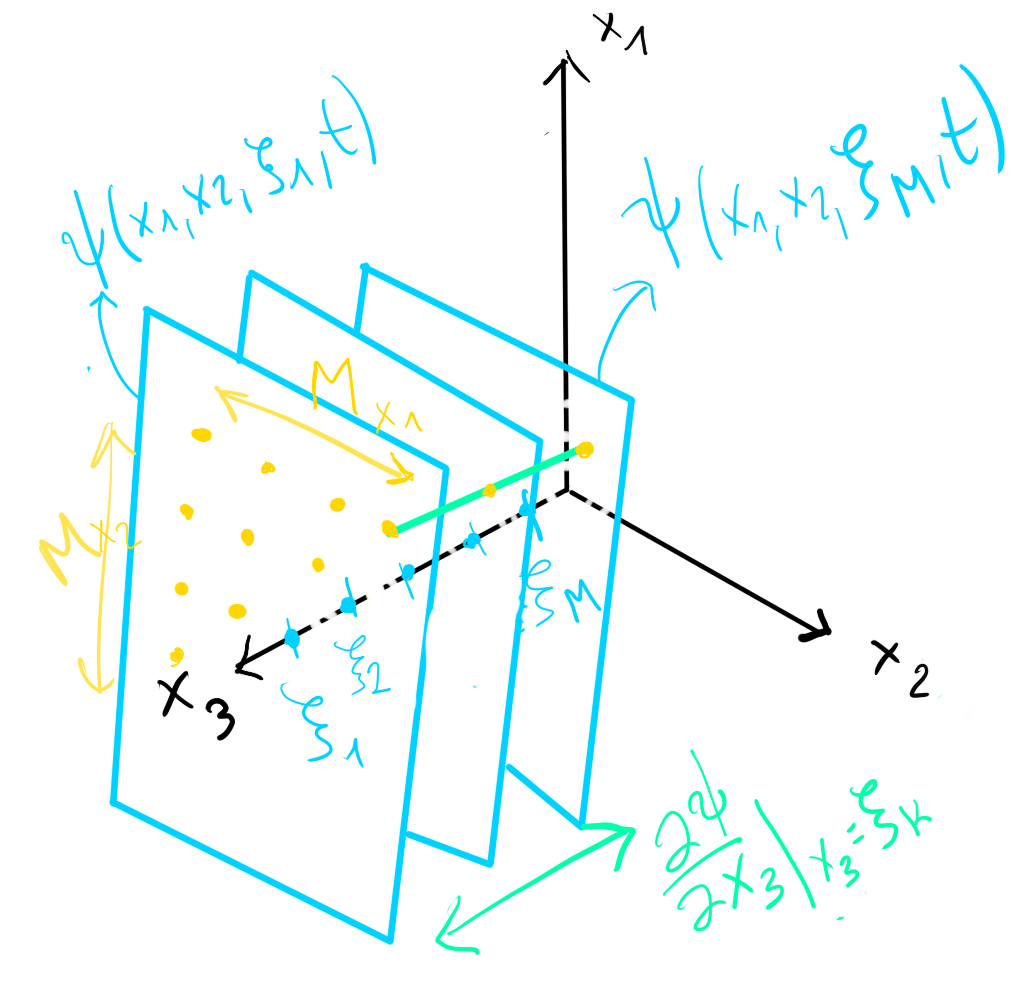
\includegraphics[width=0.5\linewidth]{hyperplaness.png}
  \caption{The $M$ hyperplanes in blue depict the $N-1$ dimensional supports of the CWF-s with a single Lagrangian degree ($x_3$). Each hyperplane is labeled by the initial position in the $x_3$ axis, the labels $\xi_j$. The yellow dots represent the $M_{x1}xM_{x2}$ discretized points of each hyperplane CWF. As it can be seen, the yellow points of the different hyperplanes are aligned, since the trajectories are fixed. This means that derivatives in the Lagrangian axis can be computed numerically at all times for any considered point in the hyperplanes.}
  \label{fig:hyperplane}
\end{figure}
\mybox{
We could do the same but instead of considering a single Lagrangian axis, we could consider two. In such a case, each CWF would have support in an affine $N-2$D manifold. Now about $O(M^2)$ CWF-s would be required, but each of them would take $O(M^{N-2})$ time to get evolved if we knew the correlation potentials. Now the derivatives to compute the correlation potentials would be required to be done in two directions, menaing we would require $O(2M^{N-2})$ threads computing each $O(M)$ operations. A total time of $O(M^{N-2})$ would be enough, at the expense of using more parallel threads.\\

If we wanted to minimize the computational time, what we could do is the following: consider all but one degree as Lagrangian, considering this way CWF-s like $\psi(x_1,x_2^\xi(t), ...,x_N^\xi(t))$, the support of which would be a line moving in $\R^N$. See Figure \ref{fig:line}. If we build a regular grid in the space $x_2,...x_N$, for each point in the grid, we could consider a line-CWF extending in $x_1$ (the labels $\xi$ of each CWf would be their positions on this initial grid).}

\mybox{ Taking $O(M^{N-1})$ line-CWFs of those (each in a different thread), we would have a value of the WF per point in the whole configuration space (considering each CWF is discretized in $O(M)$ points, we would have a regular grid for the full wave-function). Then, in order to compute the correlation potentials, we would require for each of the $O(M)$ points of the line-CWF (the Eulerian axis), the derivative in each of the $N-1$ directions of the Lagrangian axes. If there are $M^{N-1}$ CWF-s, the same $O(M^{N-1})$ threads could compute the $O(M[N-1])$ derivatives. In total a perfect parallelization in those $O(M^{N-1})$ threads would take then $O(M[N-1]+M)=O(MN)$ operations. If we assume there is an overhead per message pass between the threads, each thread needs to send and receive $O(NM)$ values, leaving a total complexity in time that is $O(MN)$ to compute a single time iteration of the full wavefunction. This is linear in time wiht increasing precision and number of spatial dimensions, but is exponential in the number of threads required for it.}

\begin{figure}[h!]
  \centering
    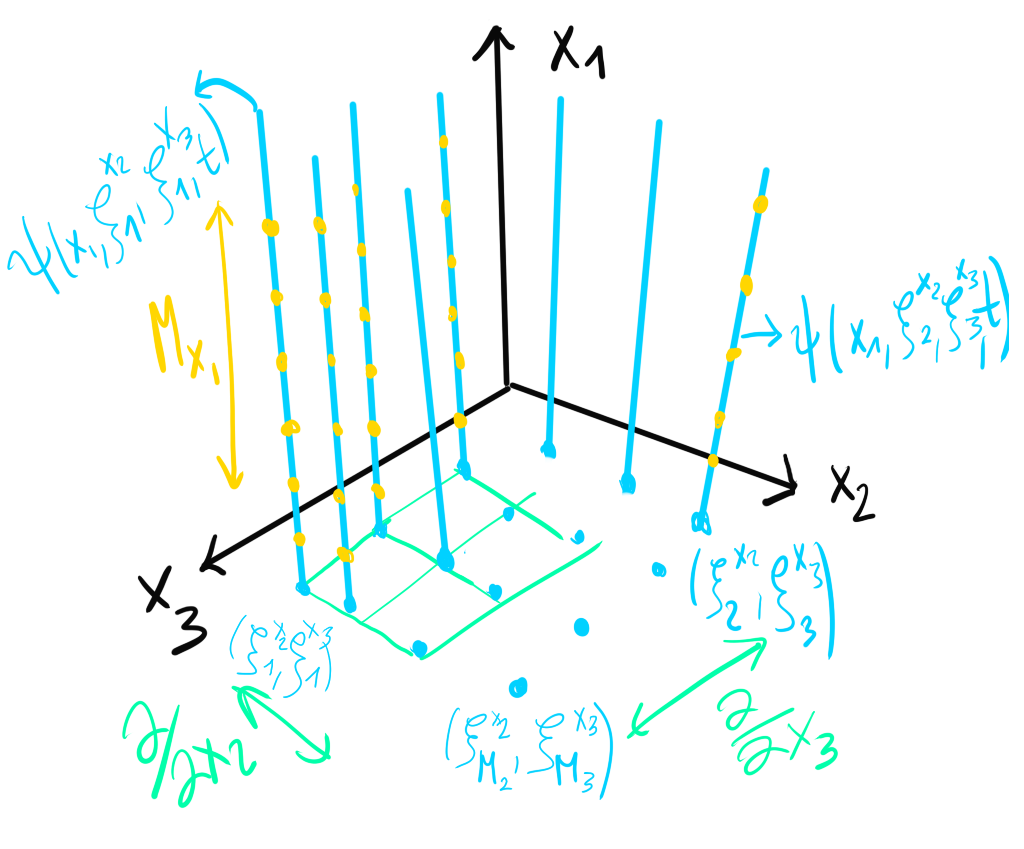
\includegraphics[width=0.5\linewidth]{rectas.png}
  \caption{In blue, the $M_{x2}xM_{x3}$ CWF-s, the supports of which are 1D manifolds. In yellow, the $M_{x1}$ discrete points we consider in each CWF. Note how the yellow points in $x_2$ and $x_3$ are aligned in a regular grid, meaning they can be used to compute numerically the derivatives in the Lagrangian directions.  }
  \label{fig:lines}
\end{figure}

\mybox{
For any intermediate arrangement of Eulerian and Lagrangian degrees of freedom, we could balance the computational complexity from temporal to spatial at will. The more Lagrangian coordinates we choose the more parallel threads will be required, but the less time it will take.\\

This approach is in principle legitimate for both the approach described in II.a.1 or II.a.2, the differences are the following ones though: the equation in II.a.1 has affine terms that impede the usage of reliable methods like the Crank Nicolson one. However, in II.a.2 we need to compute terms where we have $R$ dividing. This is prone to introduce big errors where the density is small.

}

Es la salvacion, y la unica "ventaja" de las CWF kizas. Ze sale una ecuacion lienal, solucionable de forma estable (aunke no preserve la norma, ze hay potencial complejo). Y es un mix de la full SE y la CE+HJE es un intermitx ke solo es concebible en CWF-s.
% TODO: 
- Generalize G,J zuk guzuzen beste Eulerianera 1h
- Ein Basis Set thing eta por fin harek ekuaziñoiek idatzi 3h
- Leidú Adaptive Gridsen kapituloa 
- Idatzi ALE+suggestion de hacerlas lienales haciendo trajs ke siguen la densidad? 3h
- Leidú dynamical equations for partial derivatives eta idatzi euren atala. 3h
- Leidu lo de Jacobianena eta idatzi suggestion para hacer derivadas respecto a las material coordinates. 3h
- Eing marrazkixek. 3h


\subsection*{(II.b.1) The Continuity + The Hamilton-Jacobi Equations}
If we evaluate the trajectory $\vec{y}(t;\vec{\xi})$ in the Continuity equation \eqref{CE}, we obtain:
\begin{equation}
\dv{}{t}\rho(\vec{x},\vec{y}^\xi(t),t)=-\sum_{j=1}^m\pdv{}{x_j}\qty(\rho(\vec{x}, \vec{y}^\xi(t), t) \frac{1}{m_j}\pdv{S(\vec{x}, \vec{y}^\xi(t), t)}{x_j}) - \rho(\vec{x}, \vec{y}^\xi(t),t) \sum_{j=m+1}^N \frac{1}{m_j}\pdv[2]{S(\vec{x}, \vec{y}, t)}{x_j}\Big\rvert_{\vec{x}^\xi(t)}
\end{equation}
Which is a continuity equation for $\rho(\vec{x},\vec{y}^\xi(t),t)$ with a source term $- \rho(\vec{x}, \vec{y}^\xi(t),t) \sum_{j=m+1}^N \frac{1}{m_j}\pdv[2]{S(\vec{x}, \vec{y}, t)}{x_j}\Big\rvert_{\vec{x}^\xi(t)}$ that drains or injects density as a function of the sign of the gradient of the velocity field in the Lagrangian axes (the contraction or dilation of the volume element, the determinant of the Jacobian of the density for the Lagrangian degrees). This is why the time evolution of the CWF-s is non-unitary. This was already clear in the fully Lagrangian scheme, because the density of the fluid was not a conserved quantity along the trajectories, meaning that the density that each fluid element perceives can vary in time. We actually found that the amount of density a fluid element perceived changed in time with the dilatation and contraction of the trajectory bundle, as given by the Jacobian of the mesh.

Evaluating the trajectory for the Lagrangian axes in the Hamilton-Jacobi equation \eqref{HJE} we get the ugly equation:
\begin{equation}
-\dv{}{t}S(\vec{x}, \vec{y}^\xi(t),t)=\sum_{j=1}^m\frac{1}{2m_j}\qty(\pdv{S(\vec{x},\vec{y}^\xi(t),t)}{x_j})^2-\sum_{j=m+1}^N\frac{1}{2m_j}\qty(\pdv{S(\vec{x},\vec{y}^\xi(t),t)}{x_j})^2+U(\vec{x},\vec{y}^\xi(t),t)+
\end{equation}
$$
-\sum_{j=1}^m \frac{\hbar^2}{2m_jR(\vec{x},\vec{y}^\xi(t),t)}\pdv[2]{R(\vec{x},\vec{y}^\xi(t),t)}{x_j}-\sum_{j=m+1}^N \frac{\hbar^2}{2m_jR(\vec{x},\vec{y}^\xi(t),t)}\pdv[2]{R(\vec{x},\vec{y},t)}{x_j}\Big\rvert_{\vec{x}^\xi(t)}
$$
Which is the Hamilton-Jacobi equation for the CWF, except that there are two terms extracting energy: the kinetic energy of Lagrangian frame and the quantum potential contribution due to the agglomeration in that axis.

%\subsection*{(II.b.2) The Bohmian-Newton's Second Law}
%Evaluating the trajectory $\vec{y}(t;\vec{\xi})$ in the Continuity equation \eqref{CE}, we obtain:

\subsection*{(III.b.1.2) Adaptive Grid Equations}
% como puedes controlar als trayectorias dada una monitor function, por ejemplo podrias hacer que conservasen la densidad no? OStyras esa sería muy buena! De fet para esas trayectorias saldria una continuity equation exacta! Y las CWF-s tendrian una time evolution unitaria!!!! Pa sacar cual es el velocity field que deberian seguir quizas podrias mirar cuando la Lagrangian frame equation para las trajs te da que es constante la densidad. Y creo que es cuando la derivada en el espacio de la dSdx aka la velocidad (?) es constante a lo largo de la trayectoria...Y claro como es una fk continua tb deberia funcionar ke exista esa trayectoria no? 



\subsection*{(II.c) Basis Set Expansion}
\addcontentsline{toc}{subsection}{(II.c) Basis Set Expansion}
\subsubsection*{(I.c.1) Hamiltonian and Sub-Hamiltonian Eigenstate Expansion}
\addcontentsline{toc}{subsubsection}{(I.c.1) Hamiltonian and Sub-Hamiltonian Eigenstate Expansion}
In this section we will develop an equation that will allow us the time evolution of a {\bf single} CWF, without the need of evolving several of them in parallel, at the cost of knowing the eigenstates of the Lagrangian axes!

If we recover the equation \eqref{XabEq} and the formalism we employed in its derivation, we had that the full WF could be decomposed as $\Psi(x,y,t)=\sum_{j=0}^\infty\Lambda^j(x,t)\Phi^j_x(y,t)=\sum_{j=0}^\infty \varphi_j(x,y,t)$. We defined $\Phi^j_x(y,t)$ as the transversal section eigenstates of the subsystem due to the degrees of freedom $y=(x_{m+1},...,x_N)$, which depend on the slice $x=(x_1,...,x_m)$ we are looking at. Now, if we know these eigenstates and we evaluate the wavefunction along a trajectory for the "transversal" degrees of freedom $y^\xi(t)$, we note that equation \eqref{XabEq2.5} becomes:

\begin{equation}
 i\hbar\pdv{}{t}\varphi^k(x,y^\xi(t),t)=\qty[ \varepsilon^k(x,t)+V(x,t)  -\sum_{s=1}^m\frac{\hbar^2}{2m_s}\pdv[2]{}{x_s} ]\varphi^k(x,y^\xi(t),t)+
\end{equation}
$$
+\sum_{j=0}^\infty\sum_{s=1}^m \frac{-\hbar}{2m_s}\qty( \frac{1}{\Phi^j_x(y^\xi(t),t)}\pdv[2]{\Phi^j_x(y^\xi(t),t)}{x_s}+2\pdv{}{x_s}log(\Phi^j_x(y^\xi(t),t))\qty[\pdv{}{x_s}-\pdv{}{x_s}log(\Phi^j_x(y^\xi(t),t))] )\varphi^j(x,y^\xi(t),t)
$$
Denoting $\varphi^k_\xi(x,t)=\varphi^k(x,y^\xi(t),t)$ and thus the CWF $\Psi^\xi(x,t)=\sum_j \varphi^j_\xi(x,t)$, by using the chain rule for the time derivative we get:
\begin{equation}\label{XabEq3}
 i\hbar\pdv{}{t}\varphi^k_\xi(x,t)=\qty[-\sum_{s=1}^m\frac{\hbar^2}{2m_s}\pdv[2]{}{x_s}+ \varepsilon^k(x,t)+V(x,t)   +i\hbar \dv{}{t}log(\Phi^k_x(y^\xi(t),t))]\varphi^k_\xi(x,t)+
\end{equation}
$$
+\sum_{j=0}^\infty\sum_{s=1}^m \frac{-\hbar}{2m_s}\qty( \frac{1}{\Phi^j_x(y^\xi(t),t)}\pdv[2]{\Phi^j_x(y^\xi(t),t)}{x_s}+2\pdv{}{x_s}log(\Phi^j_x(y^\xi(t),t))\qty[\pdv{}{x_s}-\pdv{}{x_s}log(\Phi^j_x(y^\xi(t),t))] )\varphi^j_\xi(x,t)
$$
This is a coupled system of {\bf linear} equations that allows the time evolution of a {\bf single CWF}, if we truncate the series $\Psi^\xi(x,t)=\sum_j \varphi^j_\xi(x,t)$ at a convenient point. Since it is linear, a Crank Nicolson like stable algorithm can be used to evolve it in a time in the order of the resolution of an $m$ dimensional Schrödinger Equation. Of course, the trick to overcome the many body problem is in that we know a priori the transversal section eigenstates $\Phi^j_x(y,t)$ for the particular potential energy. Obtaining these $N-m$ dimensional eigenstates numerically presents the same exponential nature as the full Schrödinger Equation.

However, it is really interesting to note that this is in practice the only approach that allow the exact (with no theoretical approximation) time evolution of a single CWF!



\subsubsection*{What could be the advantage of the Part Lagrangian Part Eulerian approach?}
The advantage is that we might be able to get the best of both worlds: the Eulerian and the Lagrangian.

\begin{itemize}
\item The more dimensional the CWF's Eulerian degrees are, the smaller the space for sampling the trajectories of the Lagrangian part will be. This means that the less CWF-s will be required to reproduce the full wavefunction or to achieve a certain precision in the derivatives in Lagrangian directions. However, the more computationally complex will be the CWF-s to evolve, so the problem gets more complex to be parallelized. In the limit, of $m=N$ we would recover the linear Schrödinger equation in the Eulerian frame, which scales exponentially in time with dimensions.

\item The less dimensional the CWF's Eulerian degrees, the more trajectories we will need to reconstruct the full wavefunction and to get the derivatives in the Lagrangian directions, in fact, presumably exponentially more. However, the CWF-s will be simpler to evolve and as the trajectories can (and must) be computed coupled but in parallel, the more of exponential complexity we will transfer to parallel threads. In the limit of $m=0$, we recover the fully Lagrangian frame, where we achieve the apparently highest parallelizability of the Quantum many body problem.

\item Unlike the fully Lagrangian frame, in this case, each Bohmian trajectory is accompanied by lots of wavefunction points (not just one) and therefore, interpolating the full wavefunction is way simpler, by for instance a nearest neighbour approach. Each CWF is a full $mD$ affine hyperplane of values for the wavefunction.

\item The grid is preserved in a structured manner at all times for the Eulerian degrees, while it gets unstructured for the Lagrangian axes. However, if coupled CWF-s are present, there are parts of the Lagrangian axes for one CWF that are Eulerian for the other, so there is always track of the wavefunction in all the extent of the simulation domain. The intersting thing is that the points in x of different trajectory CWF-s are always aligned, so the numerical derivatives in y or interpolations are ways impler than in a fully unstructured grid.

\item {\bf Fast and Slow Degrees of Freedom}: CWF-s provide a natural way to treat the slow degrees of freedom separated form the fast ones, like an atom nuclei from the orbiting electrons. It is common in molecular dynamics algorithm to consider classical trajectories for parts of the quantum system and quantum wavefunctions for other parts. We will see how we could do this using CWF-s in the Bohmian Newton's Equation.
\item Aproximaziñoak eitzeko de puta madre daulea
\end{itemize}



\subsection*{(III.d) Dynamic Equations for Partial Differentials}

\newpage
\section*{IV . No Continuous Fluid: Finite Tangent Universe Mechanics}
\addcontentsline{toc}{subsection}{\bf IV . No Continuous Fluid: Finite Tangent Universe Mechanics}




 


\begin{thebibliography}{1}
\addcontentsline{toc}{section}{References}

\bibitem{JordiXO}
	Oriols X, Mompart J, {\em Applied Bohmian Mechanics: From Nanoscale Systems to Cosmology} Pan Stanford, Singapore (2012)
	
%\bibitem{XO}
%	Oriols X. 2007 {\em Quantum-trajectory approach to time-dependent transport in mesoscopic systems with electron-electron interactions} Phys. Rev. Lett. 98 066803

\bibitem{Wyatt}
R. E. Wyatt, {\em Quantum Dynamics with Trajectories} (Springer, Berlin, 2006)

%\bibitem{Dev}
%	Devashish Pandey, Xavier Oriols, and Guillermo Albareda. {\em Effective 1D Time-Dependent Schrödinger Equations for 3D Geometrically Correlated Systems.} Materials 13.13 (2020): 3033.

\bibitem{nireTFGie}
	Oyanguren Xabier, {\em The Quantum Many Body Problem}, Bachelor's Thesis (2020) for the Nanoscience and Nanotechnology Degree (UAB).

\href{https://github.com/Oiangu9/The\_Quantum\_Many\_Body\_Problem\_-Bachellors\_Thesis-/blob/master/TheQuantumManyBodyProblem\_\_BachelorsThesis\_XabierOyangurenAsua.pdf}{https://github.com/Oiangu9/The\_Quantum\_Many\_Body\_Problem\_-Bachellors\_Thesis-/blob/master/TheQuantumManyBodyProblem\_\_BachelorsThesis\_XabierOyangurenAsua.pdf}

\bibitem{physicalOriols}
Norsen, T., Marian, D. \& Oriols, X. {\em Can the wave function in configuration space be replaced by single-particle wave functions in physical space?.} Synthese 192, 3125–3151 (2015). \href{https://doi.org/10.1007/s11229-014-0577-0}{https://doi.org/10.1007/s11229-014-0577-0}


\bibitem{movingGrids}
Knupp, Patrick \& Steinberg, Stanly. {\em The Fundamentals of Grid Generation.} (1993) \href{https://www.researchgate.net/publication/265361548_The_Fundamentals_of_Grid_Generation}{https://www.researchgate.net/publication/265361548\_The\_Fundamentals\_of\_Grid\_Generation} 

%\bibitem{Albareda}
%	Albareda G, Kelly A, Rubio A. {\em Nonadiabatic quantum dynamics without potential energy surfaces.} Phys Rev Materials. 2019; 3: 023803. 

%\bibitem{DATA}
%	All the animations employed for the analysis of Section 3.2 can be found in the following link:\\
%	\href{https://drive.google.com/drive/folders/1vnNDZrIYDlAhd-kVmmnVJgXmcdE2gxAV?usp=sharing}{https://drive.google.com/drive/folders/1vnNDZrIYDlAhd-kVmmnVJgXmcdE2gxAV?usp=sharing}
	
\end{thebibliography}


\end{document}
